%%%%%%%%%%%%%%%%%%%%%%%%%%%%%%%%%%%%%%%%%%%%%%%%%%%%%%%%%%%
%% Modelo DCOMP/PROCC da Universidade Federal de Sergipe %%
%%%%%%%%%1%%%%%%%%%%%%%%%%%%%%%%%%%%%%%%%%%%%%%%%%%%%%%%%%%%

\documentclass[a4paper,titlepage]{procc}

\newcommand{\etal}{et~al.}

\usepackage[brazil,english]{babel}
\usepackage{procc,epsfig}
\usepackage{times}
\usepackage{verbatim}
\usepackage{mathtools}
\usepackage{amsmath,amsfonts,amsthm}

%-------------------------- Para usar acentuacaoo em sistemas ISO8859-1 ------------------------------------
% Se estiver usando o Microsoft Windows ou linux com essa codificacao, descomente essa linhas abaixo
% e comente as linhas referentes ao UTF8
%\usepackage[latin1]{inputenc} 
% Usar acentuacao em sistemas ISO8859-1, comentar a linha com  \usepackage[utf8x]{inputenc}
%-----------------------------------------------------------------------------------------------------

%-------------------------- Para usar acentuacao em sistemas UTF8 ------------------------------------
% Para a maior parte das distribuicoes linux, usar a opcao utf8x (lembrar de comentar as linha referente a ISO8859-1 acima)
\usepackage{ucs}
\usepackage[utf8x]{inputenc}
%\usepackage[utf8]{inputenc}
\usepackage[T1]{fontenc}
%-----------------------------------------------------------------------------------------------------

% usado nas tabelas
\usepackage{multirow}
\usepackage{float}
\usepackage{graphicx,url}
\usepackage{subfig}
\graphicspath{{Figuras/}}
\usepackage{longtable} %tabelas longas, para tabelas que ultrapassam uma pagina
%\input{psfig.sty}


\usepackage{amssymb} %% Usando nas formulas matematicas


% ----------------- Para inserir codigo fonte de linguagens de programacao no documento -------------
\usepackage{listings}
\lstset{numbers=left,
stepnumber=1
firstnumber=1,
%numberstyle=\tiny,
extendedchars=true,
breaklines=true,
frame=tb,
basicstyle=\footnotesize,
stringstyle=\ttfamily,
showstringspaces=false
}
\renewcommand{\lstlistingname}{C\'odigo Fonte}
\renewcommand{\lstlistlistingname}{Lista de C\'odigos Fonte}
% ---------------------------------------------------------------------------------------------------

%\selectlanguage{portuges}
\sloppy

\begin{document}

%%%%%%%%%%%%%%%%%%%%%%%%%%%%%%%%%%%%%%%%%%%%%%%%%%%%%%%%%%%%%%%%%%%%%%%%%%%%%%%%
%% Informacoes para a Pagina de Rosto
%%
\Titulo{GERAÇÃO DE NUVEM DE PONTOS A PARTIR DE IMAGENS HDR} %\Titulo{Métodos de geração de imagens HDR}
\Autor{CLAUDIO MOTA OLIVEIRA}
\Data{\today} % Data da Defesa por extenso
\Ano{2016}
\Orientador{Prof.ª Dr.ª Beatriz Trinchão Andrade}
\UniverOrientador{Universidade Federal de Sergipe (UFS)}
\CoOrientador{Prof. Dr. Nome do Co-Orientador}
\UniverCoOrientador{Universidade Federal de Campina Grande (UFCG)}
\priAvaliador{Prof. Dr. Nome do primeiro Avaliador}
\UniverpriAvaliador{Universidade Federal de Sergipe (UFS)}
\segAvaliador{Prof. Dr. Nome do segundo Avaliador}
\UniversegAvaliador{Universidade Federal de Sergipe (UFS)}

\newpage
\cleardoublepage

\PaginadeRosto

\newpage
\cleardoublepage

%%%%%%%%%%%%%%%%%%%%%%%%%%%%%%%%%%%%%%%%%%%%%%%%%%%%%%%%%%%%%%%%%%%%%%%%%%%%%%%%%%%%%%%%
%% Dedicatoria
%% Na dissertação retire o simbolo % do bloco abaixo e crie o arquivo dedicatoria.tex 
%%
%\begin{dedicatoria}
%\input{dedicatoria.tex}
%\end{dedicatoria}

\newpage
\cleardoublepage

%%%%%%%%%%%%%%%%%%%%%%%%%%%%%%%%%%%%%%%%%%%%%%%%%%%%%%%%%%%%%%%%%%%%%%%%%%%%%%%%%%%%%%%%
%% Agradecimentos
%% Na dissertação retire o simbolo % do bloco abaixo e crie o arquivo agradecimentos.tex 
%%
%\begin{agradecimentos}
%\input{agradecimentos.tex}
%\end{agradecimentos}

\newpage
\cleardoublepage

%%%%%%%%%%%%%%%%%%%%%%%%%%%%%%%%%%%%%%%%%%%%%%%%%%%%%%%%%%%%%%%%%%%%%%%%%%%%%%%%%%%%%%%%
%% Resumo
%% Na dissertação retire o simbolo % do bloco abaixo e crie o arquivo resumo.tex 
%%
\begin{resumo} 
A visão computacional é uma área que possui como objetivo extrair informações significativas a partir de imagens, e assim possibilitar o processamento dessas informações como objetos para fins específicos como o reconhecimento de um ambiente e detecção de movimento. Um dos principais desafios desta área é a reconstrução de objetos 3D a partir de imagens, desafio este que é de grande utilidade, como ferramenta, para outras áreas do conhecimento. Este trabalho investiga a viabilidade do uso de imagens HDR (do inglês, \textit{High Dynamic Range}) para aumentar a qualidade de objetos 3D gerados a partir de imagens. Para isso foi feita a revisão da literatura sobre geração de imagens HDR a partir de imagens LDR (do inglês, \textit{Low Dynamic Range}), e sobre a obtenção de nuvem de pontos a partir de imagens. O trabalho foi dividido em duas etapas. Na primeira etapa foram estudados, implementados e comparados métodos de geração de imagens HDR. A segunda etapa do trabalho consistiu na exploração das possibilidades de uso de imagens HDR na geração de uma nuvem de pontos. Os resultados obtidos nestes experimentos foram comparados com nuvens de pontos geradas a partir de imagens LDR, demostrando assim o potencial da abordagem proposta em relação aos métodos convencionais.

\textbf{Palavras-chave:} HDR, LDR, nuvem de pontos, múltiplas exposições, pontos de inte-resse, função resposta, reconstrução 3D. 
\end{resumo}

\newpage
\cleardoublepage

%%%%%%%%%%%%%%%%%%%%%%%%%%%%%%%%%%%%%%%%%%%%%%%%%%%%%%%%%%%%%%%%%%%%%%%%%%%%%%%%%%%%%%%%
%% Abstract
%% Na dissertação retire o simbolo % do bloco abaixo e crie o arquivo abstract.tex 
%%
\begin{abstract}
Computer vision aims to extract meaningful information from images, in order to process this information as objects for specific purposes, such as environment recognition and motion detection. One of the main challenges of this area is the 3D reconstruction from images, which is very useful as a tool for other areas of knowledge. This work investigate the feasibility of using HDR (High Dynamic Range) images for increasing the quality of 3D objects generated from images. For that, it was made a literature review on generating HDR images from LDR (Low Dynamic Range) images, and about obtaining point cloud from images. The work was made in two stages. On the first stage methods for generating HDR were studied, implemented and compared. On the second stage were explored possibilities for using HDR images on point cloud generation. The results obtained on those experiments were compared with point clouds generated using LDR images, what showed the potential of the method proposed in relation to conventional methods.

\textbf{Keywords:} HDR, LDR, point cloud, multiple exposures, feature points, response function, 3D reconstruction. 
\end{abstract}

\newpage
\cleardoublepage

%%%%%%%%%%%%%%%%%%%%%%%%%%%%%%%%%%%%%%%%%%%%%%%%%%%%%%%%%%%%%%%%%%%%%%%%%%%%%%%%%%%%%%%
%% Lista de Figuras, Lista de Tabelas, Lista de Siglas e Sumario
%%
\selectlanguage{brazil}

\listoffigures
\listoftables
\ListadeSiglas
%\lstlistoflistings %lista de codigos fonte - Para inserir a listagem de codigos fonte
\renewcommand{\contentsname}{Sumário}
\Sumario

\Introducao

\newpage
\cleardoublepage

%%%%%%%%%%%%%%%%%%%%%%%%%%%%%%%%%%%%%%%%%%%%%%%%%%%%%%%%%%%%%%%%%%%%%%%%%%%%%%%%%%%%%%%%%
%% Definicao do cabecalho: secao do lado esquerdo e numero da pagina do lado direito
\pagestyle{fancy}
\addtolength{\headwidth}{\marginparsep}\addtolength{\headwidth}{\marginparwidth}\headwidth = \textwidth
\renewcommand{\chaptermark}[1]{\markboth{#1}{}}
\renewcommand{\sectionmark}[1]{\markright{\thesection\ #1}}\lhead[\fancyplain{}{\bfseries\thepage}]%
	     {\fancyplain{}{\emph{\rightmark}}}\rhead[\fancyplain{}{\bfseries\leftmark}]%
             {\fancyplain{}{\bfseries\thepage}}\cfoot{}

%%%%%%%%%%%%%%%%%%%%%%%%%%%%%%%%%%%%%%%%%%%%%%%%%%%%%%%%%%%%%%%%%%%%%%%%%%%%%%%%%%%%%%%%%
%
% Hifenizacao - Colocar lista de palavras que nao devem ser separadas e que 
% nao estao no dicionario portugues.
% As palavras do dicionario portugues ja sao separadas corretamente pelo lateX
%
\hyphenation{ Hardware Software }

%%%%%%%%%%%%%%%%%%%%%%%%%%%%%%%%%%%%%%%%%%%%%%%%%%%%%%%%%%%%%%%%%%%%%%%%%%%%%%%%%%%%%%%%%%
%% Capitulos da Dissertacao/Proposta
%% Da seguinte maneira:
%%
\chapter{Introdução} \label{introducao}
A visão computacional é uma área que possui como objetivo extrair informações significativas a partir de imagens, e assim possibilitar o processamento dessas informações como objetos para fins específicos como o reconhecimento de um ambiente, detecção de movimento entre outros \cite{ballard&brown}. Um dos principais desafios desta área é a reconstrução de objetos 3D a partir de imagens, desafio este que é de grande utilidade, como ferramenta, para outras áreas do conhecimento. Isso é mostrado nos trabalhos de Matsushigue \etal~\cite{matsushigue}, que abordou o uso de reconstrução de tomografias 3D para melhoria de diagnostico de fraturas na região do úmero, e como o trabalho de Andrade \etal~\cite{beatriz}, que usou métodos de reconstrução 3D para a preservação digital de obras de arte.


Outro exemplo de aplicação da reconstrução 3D a partir de imagens foi apresentada no método proposto por Argawal \etal~\cite{agarwal}. O método proposto aborda a reconstrução 3D sobre a escala de cidades utilizando-se de fotos disponíveis na Internet, que por sua vez, foram capturadas por pessoas aleatórias. Para isto foi usada como objeto de estudo a cidade de Roma que, por se tratar de uma cidade turística, possui milhares fotos disponíveis na Internet. Como resultado do trabalho, foi feita a reconstrução 3D do monumento do Coliseu de Roma.


De maneira geral, grande parte das técnicas de reconstrução 3D funcionam com base no mapeamento de pontos singulares existentes em diferentes imagens, denominados pontos de interesse. Com o uso de conjuntos de pontos de interesse comuns entre as imagens é possível estimar a posição deles em relação a um sistema de coordenadas tridimensional, gerando assim uma nuvem de pontos 3D.


Com base na revisão de literatura feita neste trabalho sobre obtenção de nuvem de pontos 3D a partir de imagens, evidenciou-se que grande parte dos métodos existentes utiliza-se de imagens com baixa faixa dinâmica (em inglês, Low Dynamic Range - LDR), que possuem uma resolução limitada de cores. Por outro lado existem também as imagens com alta faixa dinâmica (em inglês, High Dynamic Range - HDR), que possuem maior resolução de cores.

Sob o ponto de vista de acessibilidade, o uso de imagens LDR é explicado pelo fato de que câmeras com sesores capazes de capturar imagens HDR serem muito caras e assim pouco acessíveis. Porém sob o ponto de vista de qualidade, as imagens HDR possuem maior quantidade de informações do cenário em relação a uma imagem LDR. Um exemplo disso, seria um cenário de uma sala pouco iluminada, que possui uma janela ao fundo a qual mostra o céu de um dia ensolarado. Ao capturar uma imagem deste ambiente com uma câmera LDR, o fotógrafo terá que ajustar as configurações da câmera, para escolher qual parte da cena será melhor registrada (os móveis da sala ou o céu ensolarado). Já para uma câmera HDR todas as partes da imagem seriam propriamente registradas, uma vez que esta possui uma maior faixa de representação de cores.


Trabalhos publicados na literatura, propoem métodos para união de um conjunto imagens LDR em uma imagem HDR. O uso destas técnicas se mostra uma alternativa economicamente viável para obter imagens de boa qualidade, com alta faixa dinâmica.


Assim como no trabalho feito por Kontogianni~\etal~\cite{hdr3d}, o trabalho descrito neste documento possui como hipótese a ideia que um conjunto de imagens HDR têm o potencial de identificar mais pontos de interesse que um conjunto de imagens LDR, tendo em vista que o primeiro possui mais informação do ambiente que o segundo. Neste contexto, este trabalho visa verificar a viabilidade de implementação de um método para obtenção de nuvem de pontos a partir de imagens HDR. Espera-se que com isso seja possível extrair mais pontos de interesse e reconstruir nuvens de pontos com maior resolução de maneira acessível. Para que este processo possa ser realizado com um baixo custo em relação ao equipamento utilizado, se faz necessário o uso das técnicas de união de imagens LDR para geração de imagens HDR.

\section{Objetivo} \label{introducaoObjetivo}

O objetivo deste trabalho é verificar se o uso de imagens HDR, obtidas utilizando conjuntos de imagens LDR, gera nuvens de pontos mais densas em relação às nuvens de pontos geradas a partir de imagens LDR.

\section{Metodologia} \label{introducaoMetodo}

Para que seja possível alcançar o objetivo, este trabalho é dividido em duas etapas:

\begin{itemize}
\item Geração de imagem HDR:

Nesta etapa métodos de geração de imagens HDR são estudados, implementados e comparados para que sejam determinados os métodos que serão utilizados na próxima etapa.
\item Geração de nuvem de pontos:

Nesta etapa são utilizados métodos para geração de nuvem de pontos a partir de imagens, para que assim sejam realizadas as comparações inicialmente propostas.
\end{itemize}
	
\chapter{Conceitos Básicos} \label{conceitos}
	Este capítulo aborda conceitos fundamentais para a compreensão dos métodos de geração de imagens HDR e obtenção de nuvem de pontos, que serão abordados nos capítulos posteriores.
	
\section{Faixa Dinâmica} \label{conceitoFaixa}
    Cada imagem digital possui uma certa quantidade de bits para representação das cores de cada um de seus pixels. A maior parte das câmeras convencionais do mercado geram imagens com pixels que são representados por 8 bits em cada canal de cor, o que resulta numa faixa de 256 valores possíveis. Quando uma imagem possui esta faixa de representação de cores esta é chamada de imagem com baixa faixa dinâmica (em inglês, Low Dynamic Range - LDR) por possuir um intervalo relativamente curto de valores para representar as cores capturadas em uma cena. Quando uma imagem possui uma faixa maior de valores para representação de cores é denominada imagem com alta faixa dinâmica (em inglês, High Dynamic Range - HDR). As imagens HDR geralmente representam as cores em ponto flutuante, o que diminui a deterioração cumulativa ao efetuar operações sucessivas sobre a imagem. Além disso, estas imagens conseguem representar melhor as cenas capturadas em relação a uma imagem LDR, por possuírem mais bits para representação das cores.
    
    Supondo uma cena com áreas bem iluminadas, outras com iluminação moderada e outras com baixa iluminação, ao captar uma imagem LDR desta cena muito provavelmente informações das áreas com extremos de iluminação (pouco/muito iluminadas) serão perdidas. Isto acontece devido ao fato da imagem não ter uma faixa de valores suficiente para representar tanto os níveis altos como os níveis baixos de iluminação desta cena. Por outro lado, ao captar uma imagem HDR desta mesma cena mais detalhes das zonas claras e escuras serão registrados sem perdas significativas.
	
\section{Função Resposta de uma Câmera} \label{conceitoFR}
	Uma câmera digital é composta de uma matriz de elementos sensores de luz. No processo de captura de uma imagem, cada sensor pode ser considerado uma função $f$ que recebe como entradas $x$ e $t$. A entrada $x$ representa o valor de irradiação de luz que incide sobre o sensor, e $t$ representa o período de tempo que esta incidência persiste. Esta função tem como saída um valor geralmente inteiro $p$, que é o valor do pixel. $f$ é chamada de função resposta da câmera e idealmente ela pode ser descrita pela seguinte equação:
	
	
\begin{align} \label{eqConceitoFR1}
          f(x,t) &= p
\end{align}

	Porém, no mundo real há a presença de ruídos, advindos de diversas fontes, que distorcem os sinais tanto de entrada quanto de saída da câmera. Devido a isso, a equação \ref{eqConceitoFR1} pode ser modificada para a seguinte equação que discrimina os ruídos:

\begin{align} \label{eqConceitoFR2}
						f (x, t, R_a) = p + R_b
\end{align}

Onde
\begin{itemize}
	\item $R_a$ é a abstração dos ruídos advindos do meio, como ruído térmico.
	\item $R_b$ é a abstração dos ruídos gerados na conversão do sinal analógico para digital, como corrente de escuro.
\end{itemize} 
		
	Vale atentar que o valor de iluminação $x$ também é influenciado pela abertura do obturador, mas este trabalho considera que a abertura do obturador irá permanecer constante, pois qualquer mudança da abertura do obturador influenciará no foco da câmera. 
	
	Em geral, os algoritmos de geração de imagens HDR se utilizam da inversa da função resposta da câmera para compor uma função $g$ de forma que, dado um pixel $p$ e o tempo de exposição $t$, seja possível estimar o valor de iluminação $x^*$ que o gerou este pixel.

\begin{align} \label{eqConceitoFR3}
	g(p, t) = x^*
\end{align}
	
	Um dos problemas em relação a esta abordagem é que a confiabilidade dos pixels varia de acordo com o tempo de exposição \cite{robertson}, além disso, cada pixel $p$ possui um ruído agregado a ele. Assim, cada método de geração de imagens HDR trata estes problemas de maneira específica.
	
	Outro problema é que, na prática, o usuário da câmera geralmente não possui nenhuma informação sobre a função resposta da câmera que está utilizando. Devido a isso alguns autores dos métodos de geração de imagens HDR também propõem métodos de inferência da função resposta de uma câmera a partir das imagens capturadas por ela.

\section{Eixo Logarítmico} \label{conceitoGaussiana}

	Um conceito bastante abordado nos métodos de geração de imagem HDR é o uso do eixo logarítmico. Alguns métodos utilizam este conceito para ressaltar a confiabilidade que um valor de pixel representa, levando o mesmo a ter um maior ou menor peso na geração da imagem HDR.
	
	O eixo logarítmico é um eixo no qual cada graduação possui uma razão de $10$ unidades em relação a graduação anterior. A Tabela \ref{tabConceitosEixo} ilustra a variação dos valores nos eixos linear e logarítmico.
	
\begin{table}[H]
  \centering
  \caption{Progressão dos eixos}
  \label{tabConceitosEixo}
  \begin{tabular}{l|l|l|l|l}
    \hline
    Graduação           & 1º & 2º & 3º  & 4º   \\
    \hline
    Valor (linear)      & 0  & 1  & 2   & 3    \\
    \hline
    Valor (logarítmico) & 1  & 10 & 100 & 1000 \\  
    \hline
  \end{tabular}
\end{table}
	
	A Figura \ref{figConceitoEixo} mostra uma mesma função resposta representada em um eixo linear (\ref{figConceitoEixoA}) e logarítmico, respectivamente (\ref{figConceitoEixoB}).
	
\begin{figure}[H]
  \centering
  \subfloat[Linear]
  {
    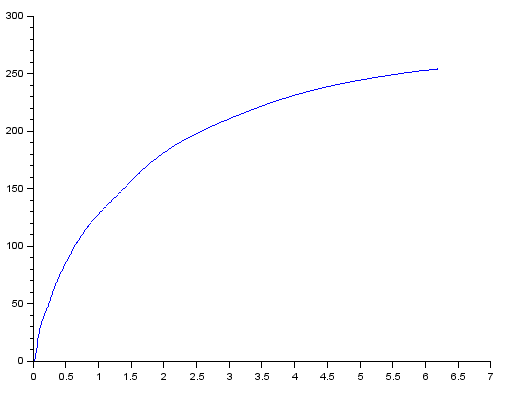
\includegraphics[height=6cm]{Fr-linear-azul}
    \label{figConceitoEixoA}
  }
  \quad %espaco separador
  \subfloat[Logarítmico]
  {
    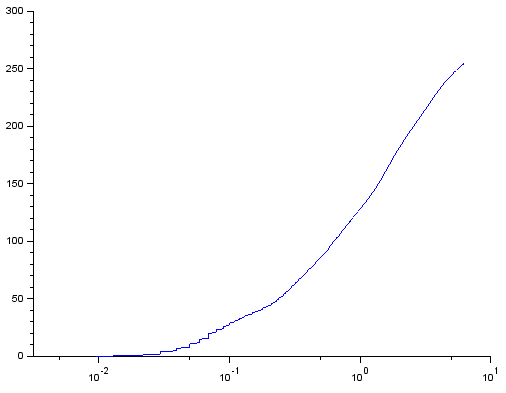
\includegraphics[height=6cm]{Fr-log-azul}
    \label{figConceitoEixoB}
  }
  \caption{Funções resposta e suas representações em diferentes eixos.}
  \label{figConceitoEixo}
\end{figure}

	A importância do eixo logarítmico para os métodos de geração de imagens HDR se dá por conta de uma suposição assumida por alguns dos autores. Segundo Mann~\cite{mann} e Robertson~\cite{robertson}, a derivada da função resposta da câmera num eixo logarítmico possui relação direta com a confiabilidade que um pixel possui, i.e, quanto maior o valor de confiabilidade menor o ruído associado ao pixel. O cálculo da derivada do ponto de uma função em relação ao eixo logarítmico é dado pela seguinte equação:
	
\begin{align} \label{eqConceitoLog1}
          y^,_{log}(x) = \frac{dy}{dx}.\frac{x}{log(e)}
\end{align}

\section{Similaridade Bidirecional} \label{conceitoSimilaridadeBidirecional}
	A Similaridade Bidirecional \cite{simakov} é um método de maximização das similaridades entre dois sinais $S$(fonte) e $T$(destino), que se utiliza de um conjunto de fragmentos de ambos os sinais para definir a similaridade tanto em relação à sua coerência quanto à completude das informações.
	
	Uma imagem $T$ é dita coerente em relação a outra imagem $S$ quando todo fragmento $P_i$, pertencente a $T$, está contido em $S$. Por outro lado, se $T$ contém todos os fragmentos de $S$, então é dita completa em relação a $S$.
	
	O método maximiza a similaridade visual por meio da minimização da seguinte função:
	
\begin{align} \label{eqConceitoSimilaridade}
          d(S,T) = \frac{1}{N_S}\sum\limits_{P \subset S}{\underset{Q \subset T}{min}~D(P,Q)} + \frac{1}{N_T}\sum\limits_{Q \subset T}{\underset{P \subset S}{min}~D(Q,P)}
\end{align}

Onde
\begin{itemize}
	\item $N_S$ e $N_T$ são os números de fragmentos de $S$ e de $T$ respectivamente.
	\item $D(,)$ representa a distância, i.e., dissimilaridade entre dois fragmentos. 
\end{itemize} 
	

 \section{Relaxação de Gauss-Seidel} \label{conceitoGauss-Seidel}
	Consiste num método para resolução de sistemas de equações com múltiplas variáveis simultaneamente de forma iterativa. O método consiste em, a partir de valores iniciais especulados, inferir o valor de uma variável e, com este valor encontrado, estimar o valor da próxima variável. O processo é repetido iterativamente para todas as variáveis de maneira cíclica até atingir uma determinada condição de convergência. Mais informações sobre o método estão disponíveis no livro de Ruggiero e Lopes~\cite{livroCalculoNumerico}.
	

\section{Spline Cúbica} \label{conceitoSpline}

	Spline cúbica é um método de interpolação que possui como principal característica a geração de uma função contínua, com primeira e segunda derivadas também contínuas. A interpolação consiste em, dado um conjunto de pontos $S$ = $\{(x_i,y_i)\}$, obter uma função $y(x)$ que contenha todos estes pontos. Para isso considera-se que cada intervalo entre dois pontos consecutivos são funções polinomiais de terceiro grau. A partir de premissas definidas em relação ao primeiro e último ponto, são descobertos os valores das funções de cada intervalo. Mais informações sobre o funcionamento deste método podem ser encontradas no livro de Ruggiero e Lopes~\cite{livroCalculoNumerico}.
	
	
	
	

\chapter{Obtenção de Imagens HDR a Partir de Imagens LDR} \label{metodos}
Neste capítulo será mostrada a pesquisa bibliográfica e implementação de métodos de geração de imagens HDR a partir de um conjunto de imagens LDR. O principal objetivo deste capítulo é comparar os métodos existentes na literatura, afim de definir um método viável para geração de imagens HDR que servirão de entrada para a próxima etapa do projeto.

\section{Revisão Bibliográfica} \label{revisaoPontos}

Dentre os principais assuntos que se relacionam ao tema deste capítulo, pode-se destacar a obtenção de pontos de interesse de imagens HDR e a geração de nuvens de pontos. Nesta seção serão abordados trabalhos da literatura que se relacionam com estes temas.

Kontogianni~\etal~\cite{hdr3d} apresentaram um estudo sobre a diferença entre imagens LDR e HDR na obtenção de pontos de interesse. A motivação do trabalho foi importância da preservação da herança cutural e arquitetural que pode ser feita através da recontrução 3D, e com isso a necessidade de alta precisão e preservação dos detalhes no processo. A hipótese foi que o uso das imagens HDR implicaria num maior número de pontos de interesse, que por sua vez agregariam mais informação para a recontrução 3D das cenas. Na implementação foram geradas imagens HDR a partir de conjuntos de imagens LDR, seguida pelo \textit{tone mapping} da imagem HDR gerada, para assim passá-la como entrada dos algoritmos de obtenção de pontos de interesse. Os resultados mostraram que o uso das imagens processadas obteve um aumento significativo do número de pontos de interesse encontrados em relação às imagens LDR.

P\v{r}ibyl~\etal~\cite{hdr3d2} também apresentaran um trabalho que verifica a serventia de técnicas HDR para obtenção de pontos de interesse em condições extremas de iluminação, i.e, que possui áreas bem muito iluminadas e áreas pouco iluminadas. Assim como Kontogianni~\etal~\cite{hdr3d}, utilizou-se de técnicas de \textit{tone mapping} sobre as imagens HDR para então usá-las como entrada de métodos de obtenção de pontos de interesse. Seus resultados mostraram que o uso das imagens processadas aumentou a taxa de repitibilidade dos pontos de interesse significativamente.

%Lowe~\cite{sift} introduziu um método para detecção, descrição e extração de pontos de interesse %denominado SIFT(textit{Scale Invariant Feature Transformation}). Os pontos de interesse extraídos %por este método são invariantes a escala, rotação e parcialmente a mudança de iluminação.
%
O trabalho mostrado por Wu \cite{visualSFMBA} introduz uma nova técnica de reconstrução 3D a partir de múltiplas imagens. A partir desta foi possível diminuir a complexidade da obtenção de pontos 3D. Este algoritmo é utilizado como parte do software VisualSFM~\cite{visualSFM} que será utilizado neste trabalho.


\section{Métodos HDR Selecionados} \label{metodos}
Nesta seção serão abordados os métodos de geração de imagens HDR a partir de imagens LDR escolhidos para este trabalho. Cada subseção tratará um método, mostrando aspéctos teóricos, implementação e resultados obtidos, assim como discussões sobre tópicos de interesse. Nas seções que seguem serão abordados e comparados os métodos de geração de imagens HDR dos seguintes autores:

\begin{itemize}
\item Mann e Picard: Por se tratar de um método clássico, frequentemente citado em trabalhos da área podendo ser usado como base para comparação. Além de se tratar de um método simples que aborda apenas a mudança no tempo de exposição das imagens LDR para geração de imagens HDR, e ao mesmo tempo se mostra suficiente para o objetivo final deste trabalho.
\item Robertson \etal: Por se tratar de um método mais elaborado que, além de abordar a mudança no tempo de exposição, leva em consideração aspectos de erro relativos a ruídos na aquisição das imagens LDR. 
\item Sen \etal: Por se tratar de um método robusto quanto ao movimento da câmera. Característica essa bastante importante para aplicações não profissionais, pois manter a câmera totalmente estática entre a captura das imagens é um fator limitante.
\end{itemize}


\subsection{Base de Imagens e Visualização} \label{metodoBaseImg}

Para a geração das imagens HDR nos métodos das próximas seções, será utilizada a base de imagens LDR apresentada nesta seção. Essa base de dados consiste num conjunto de cenas, cada uma possuindo regiões bem iluminadas e regiões pouco iluminadas. Cada cena foi registrada por um conjunto de imagens LDR, que diferem apenas em tempo de exposição, e cada imagem busca registrar uma faixa de iluminação específica da cena. Com isso visa-se verificar a eficiência de cada método em gerar imagens HDR dessas cenas.

É importante salientar que, apesar de pouco, o movimento entre a captura das imagens LDR de cada cena da base de dados existe. Esse foi um fator limitante neste trabalho, devido aos equipamentos disponíveis para uso. Outro fator limitante devido ao equipamento utilizado foi o uso de imagens no formato JPG, que possui compressão com perda de informações.

\subsubsection{Cena da Didática} \label{cenaDidatica}

\begin{figure}[H]
  \subfloat[Tempo de exposição de $0.002s$.]
  {
    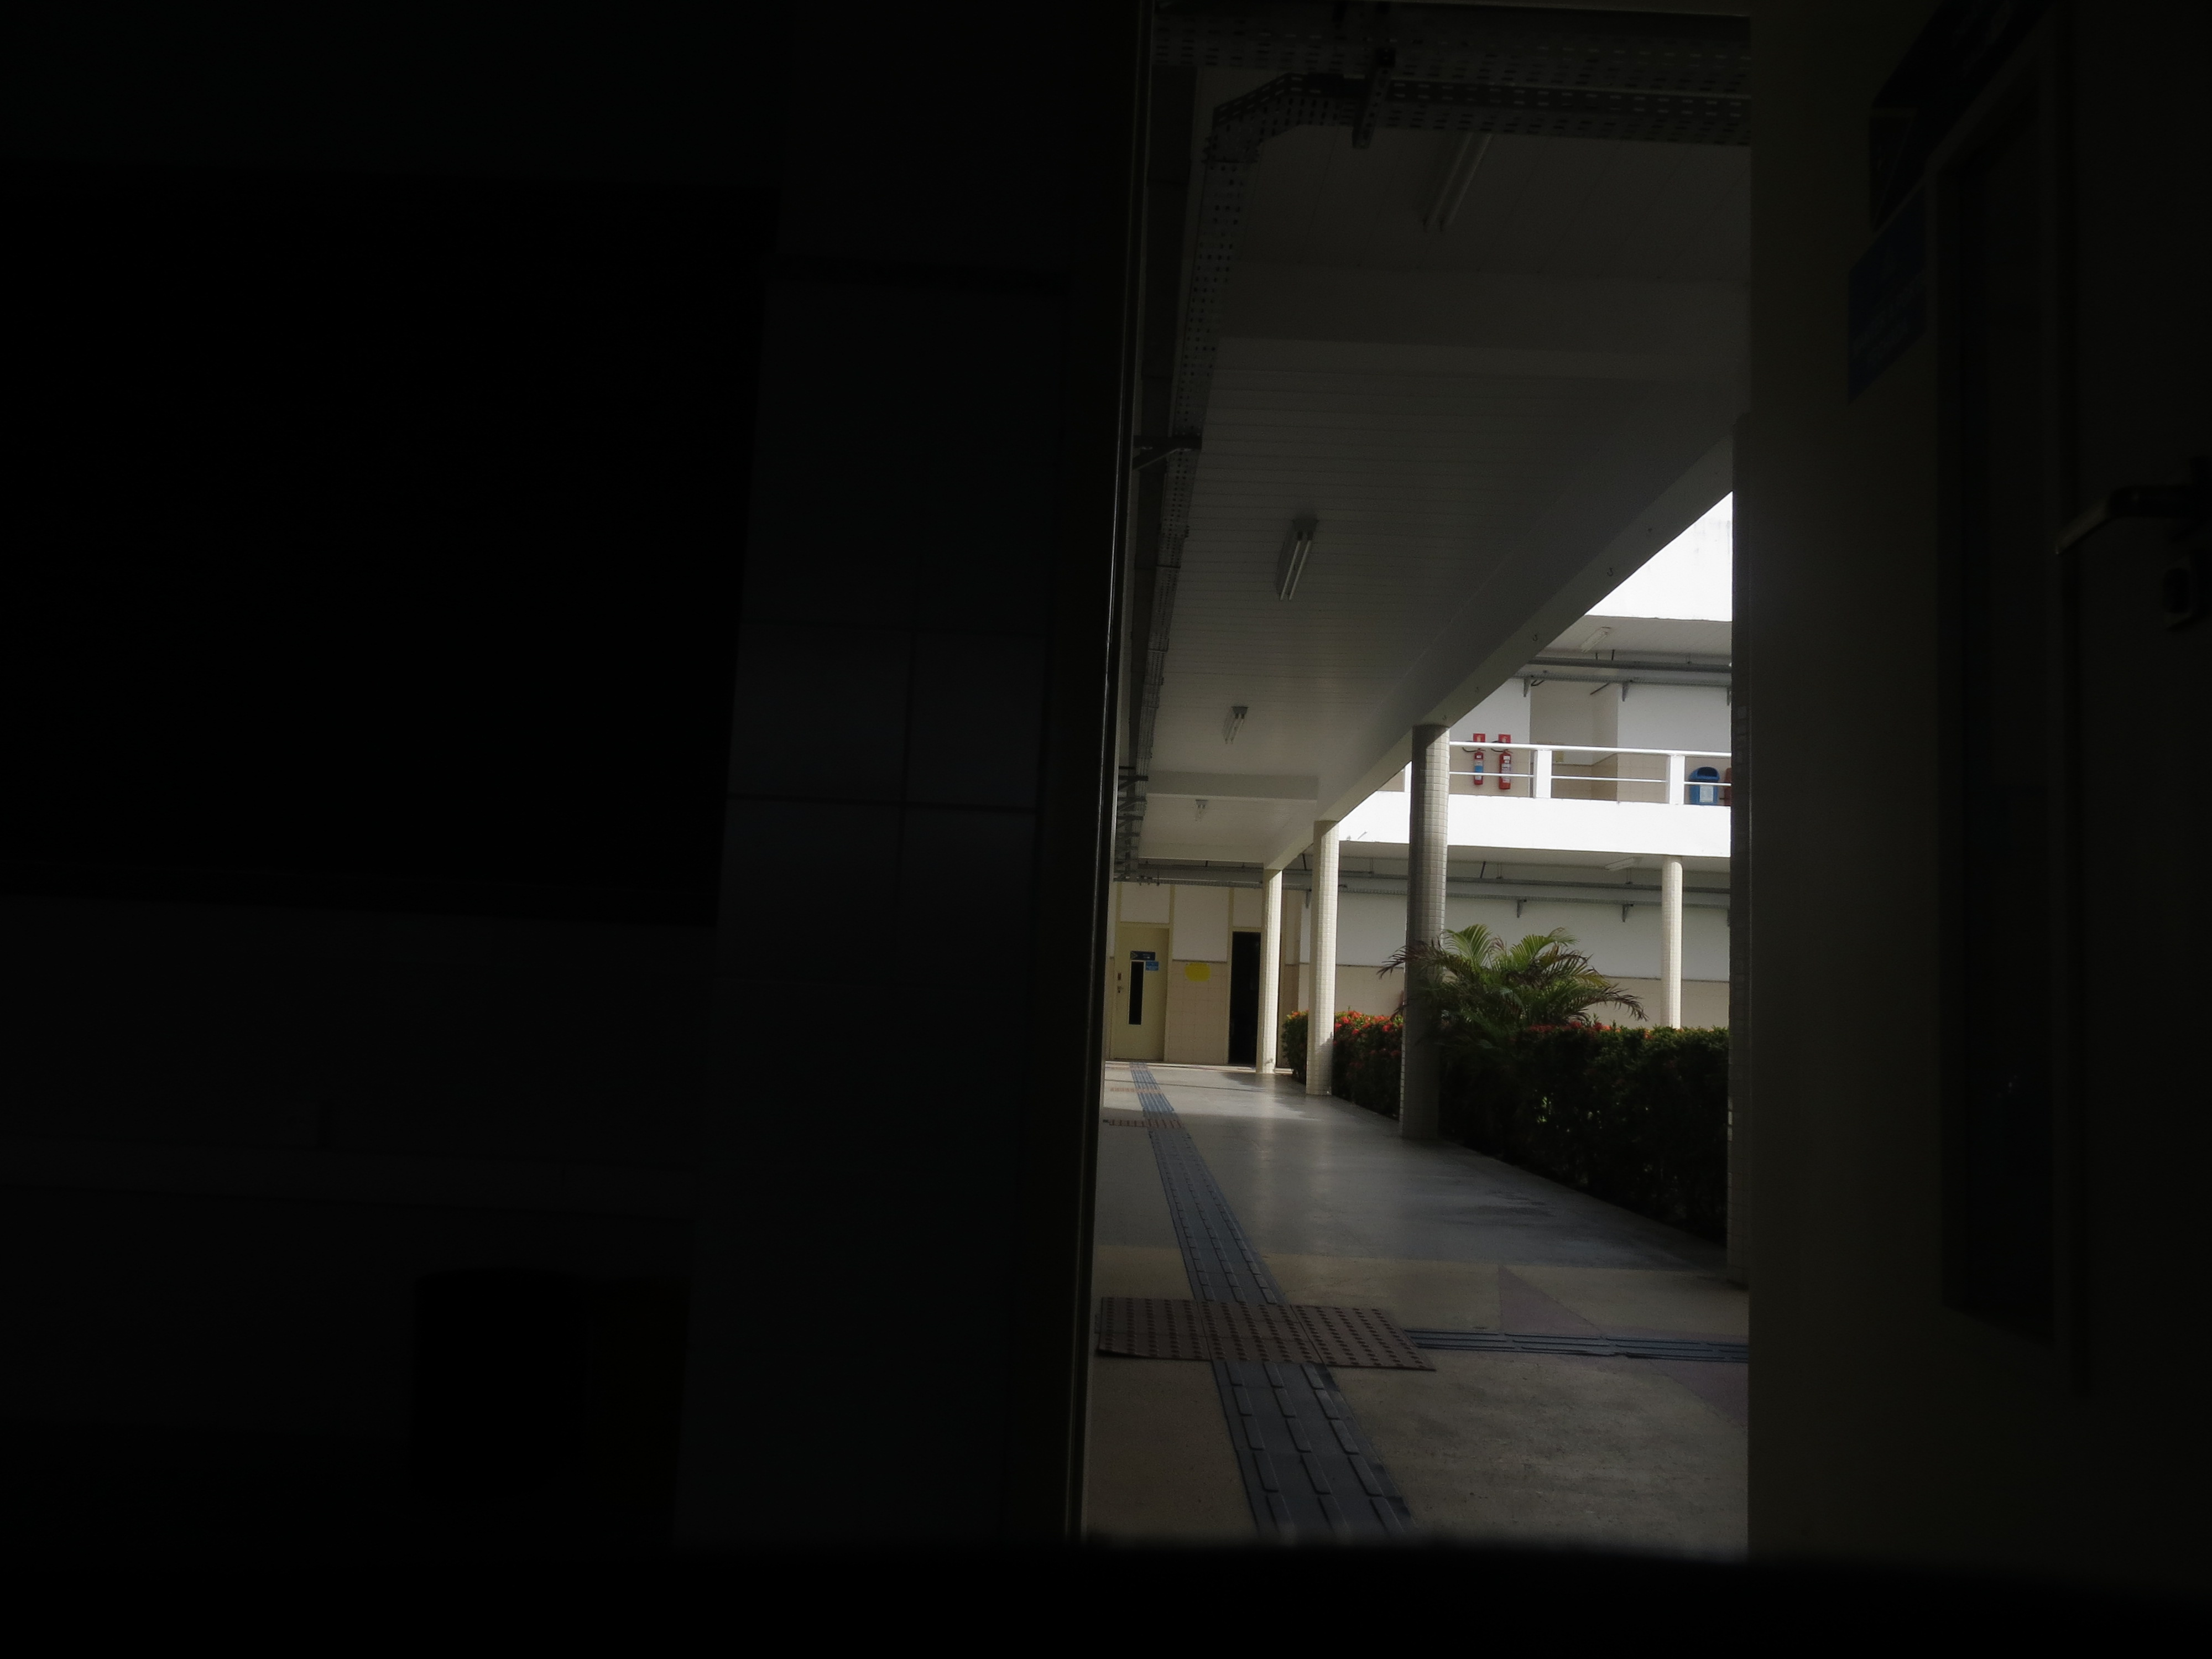
\includegraphics[height=4cm]{CenaDidatica/1}
    \label{figBaseDidaticas1}
  }
  \quad %espaco separador
  \subfloat[Tempo de exposição de $0.005s$.]
  {
    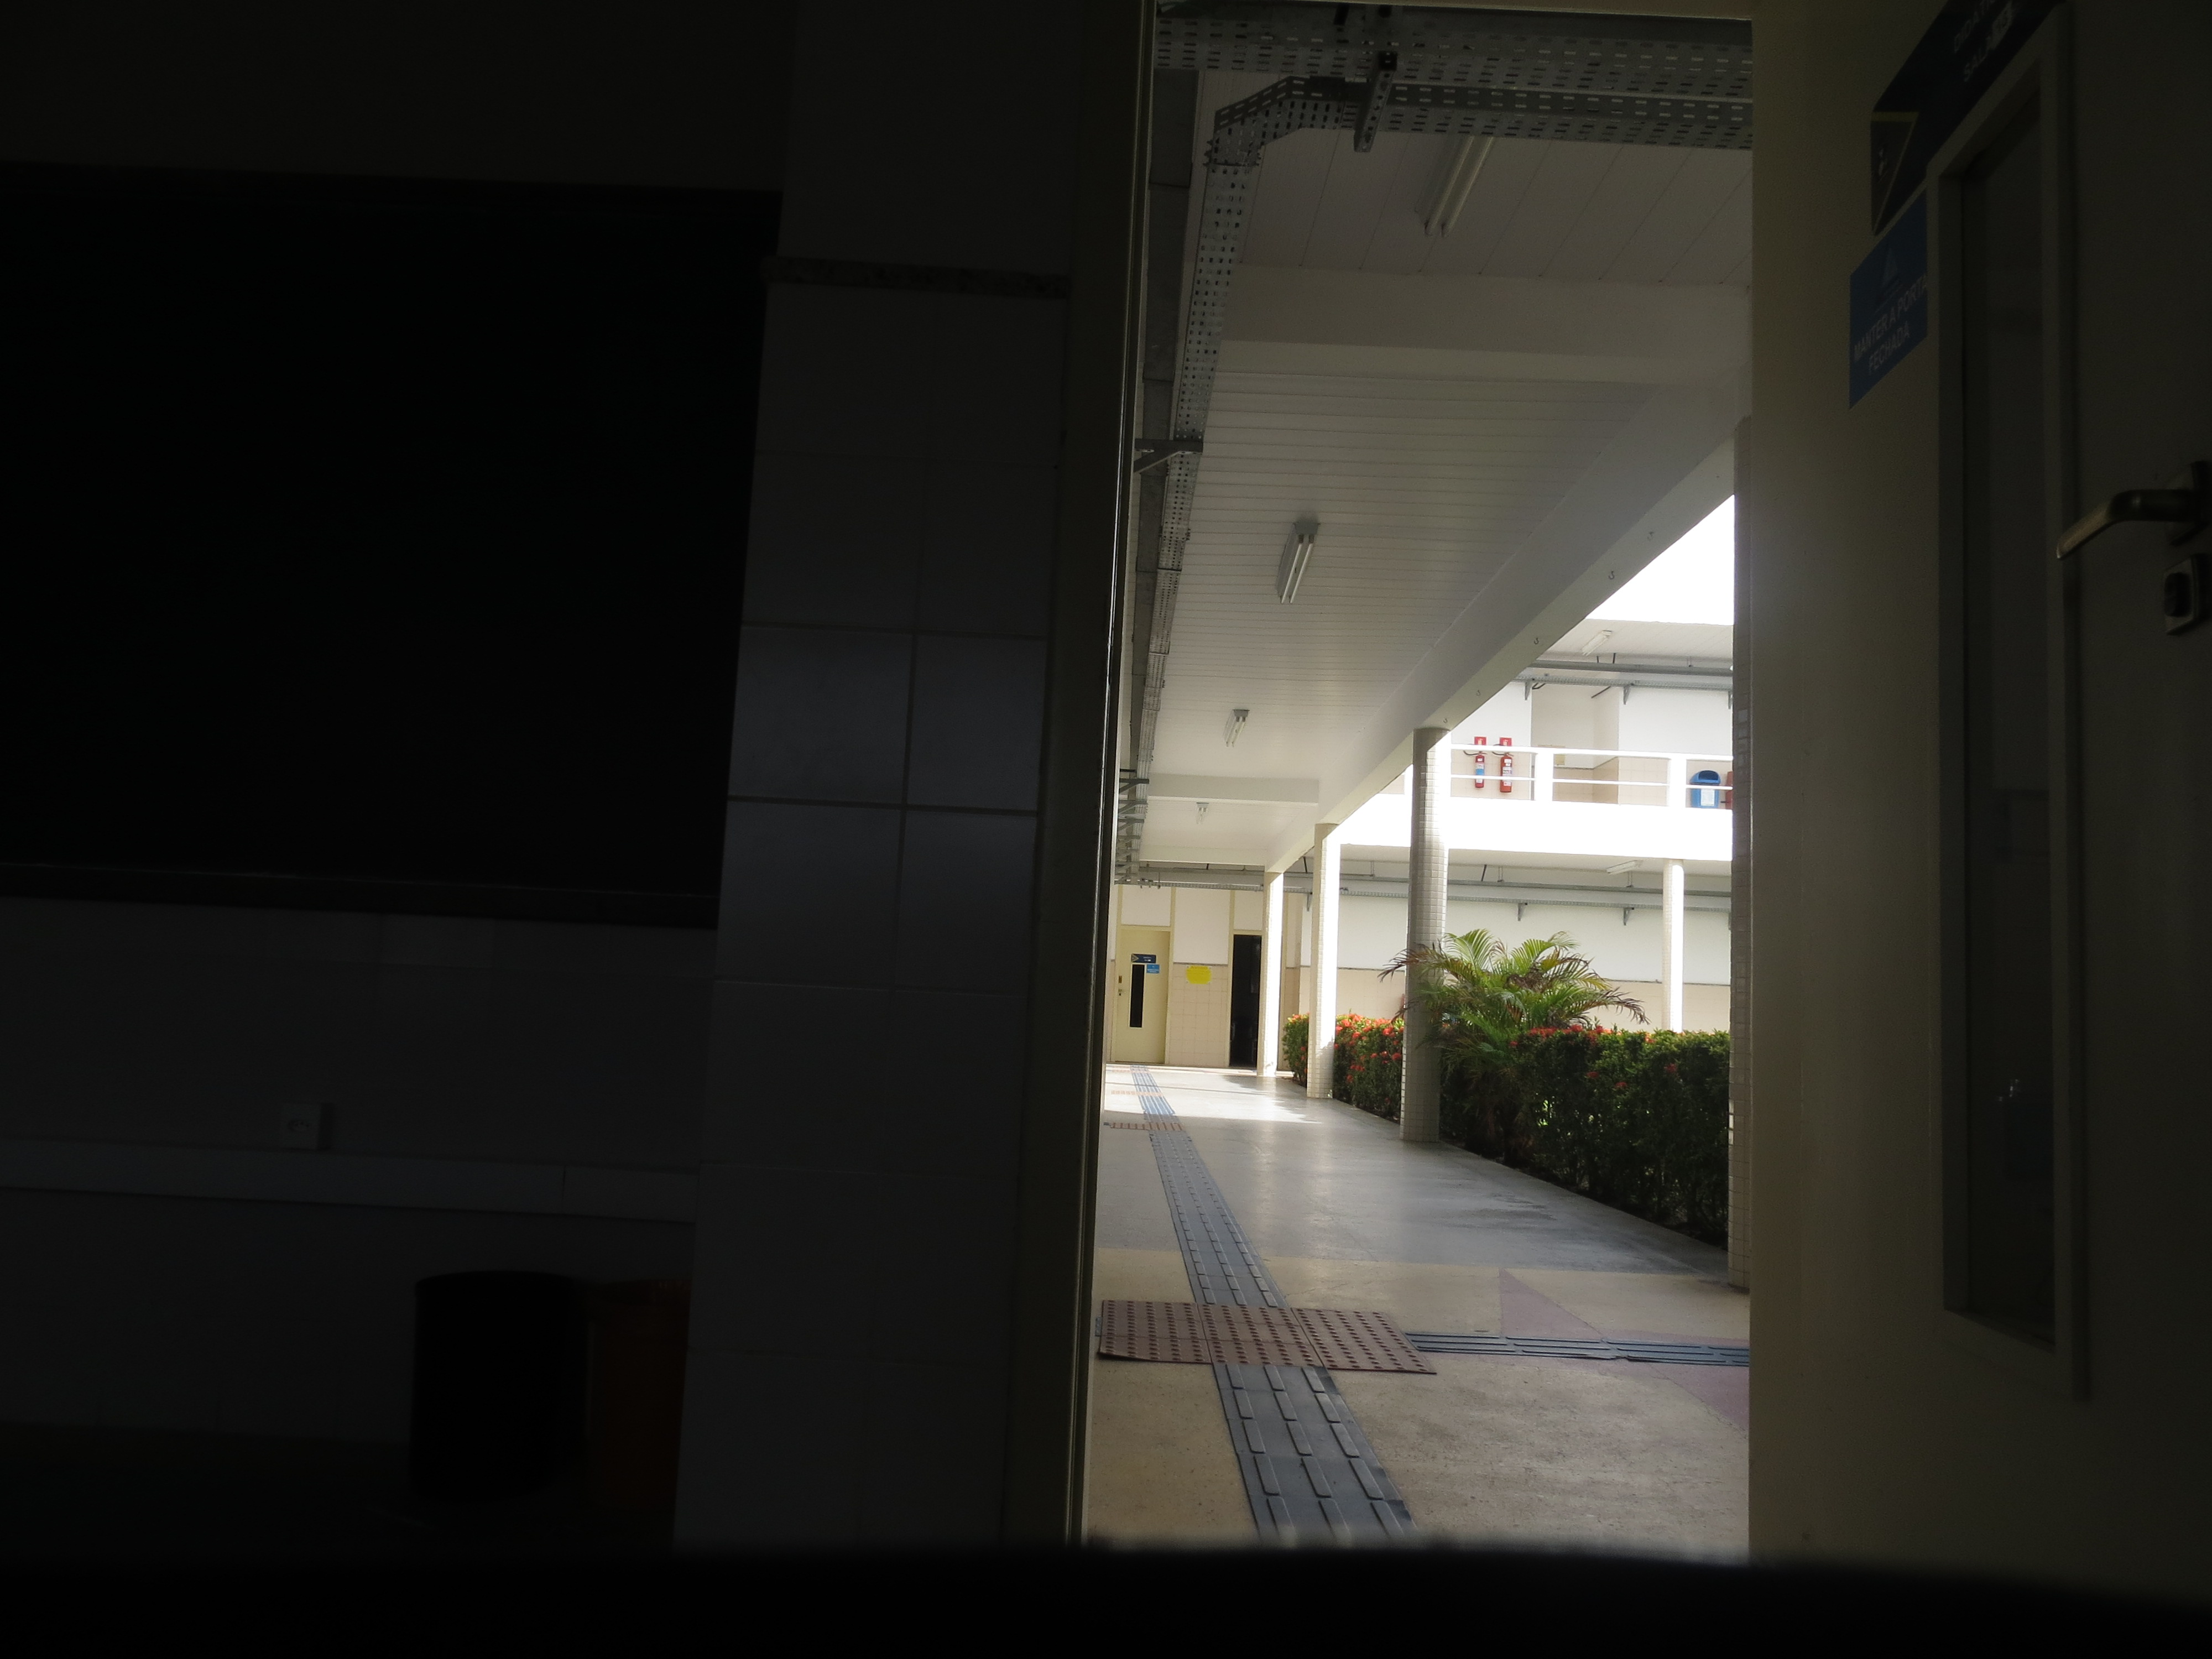
\includegraphics[height=4cm]{CenaDidatica/2}
    \label{figBaseDidaticas2}
  }
  \quad %espaco separador
  \subfloat[Tempo de exposição de $0.0167s$.]
  {
    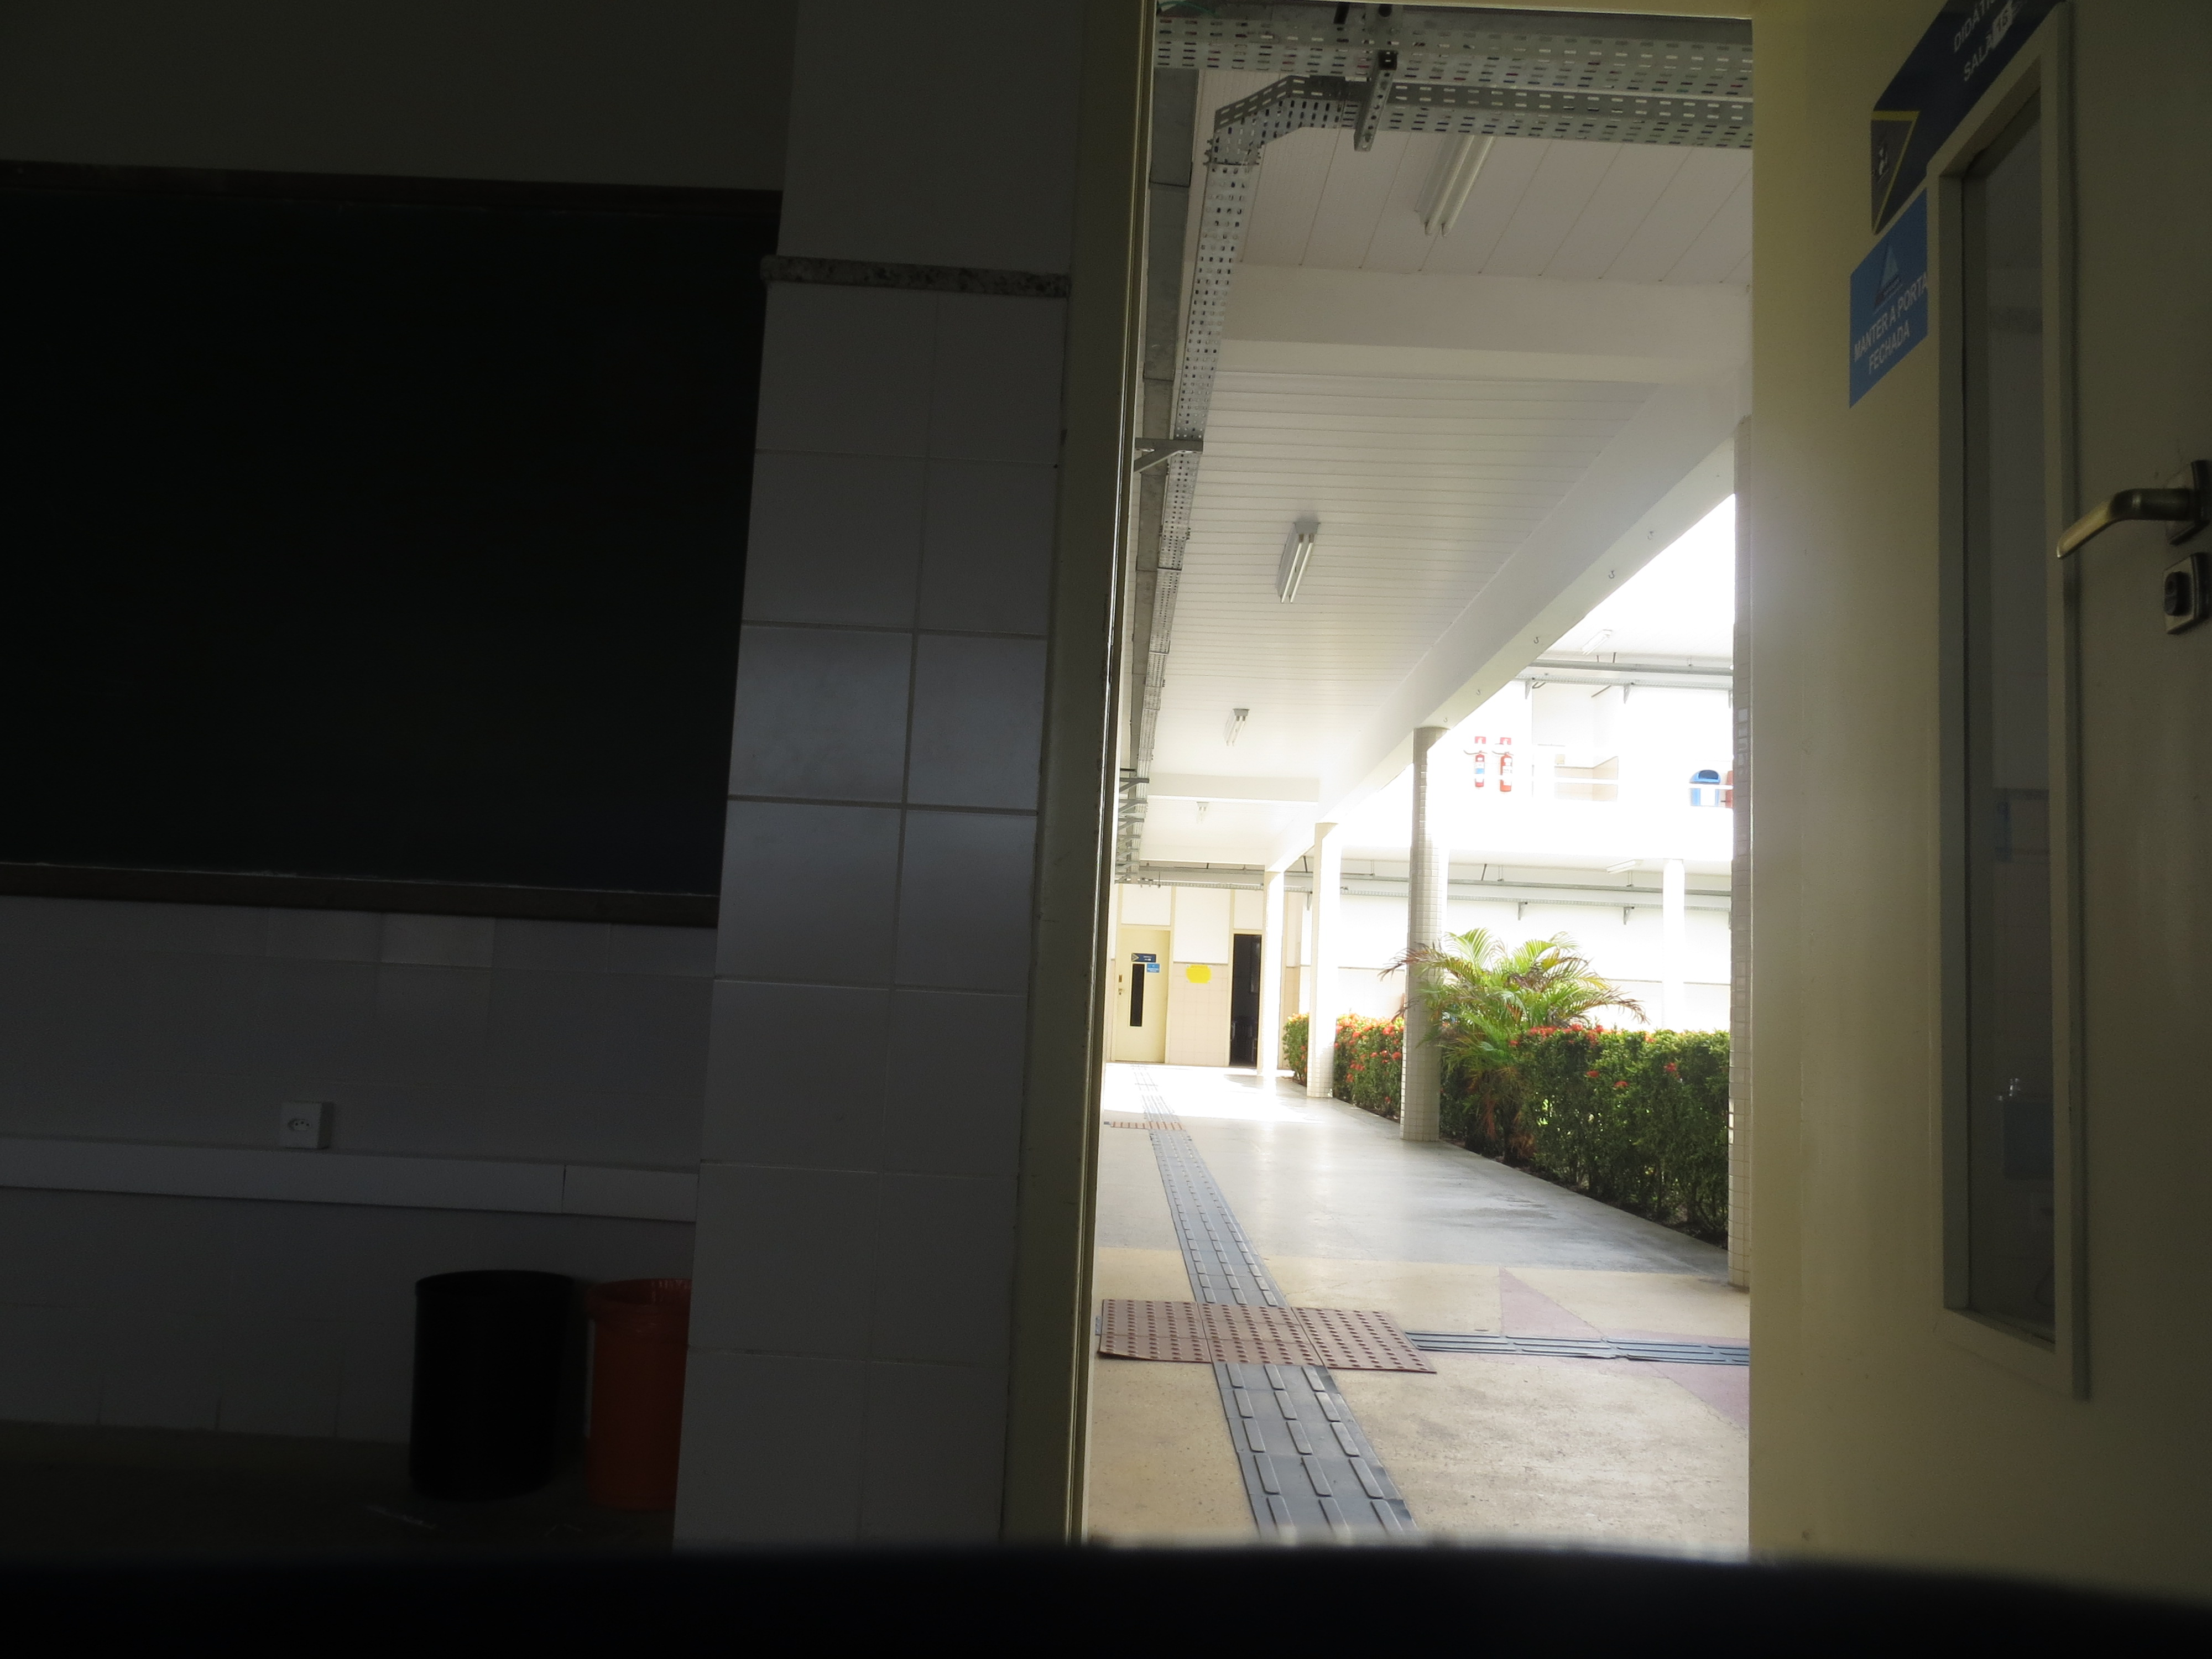
\includegraphics[height=4cm]{CenaDidatica/3}
    \label{figBaseDidaticas3}
  }
  \quad %espaco separador
  \subfloat[Tempo de exposição de $0.04s$.]
  {
    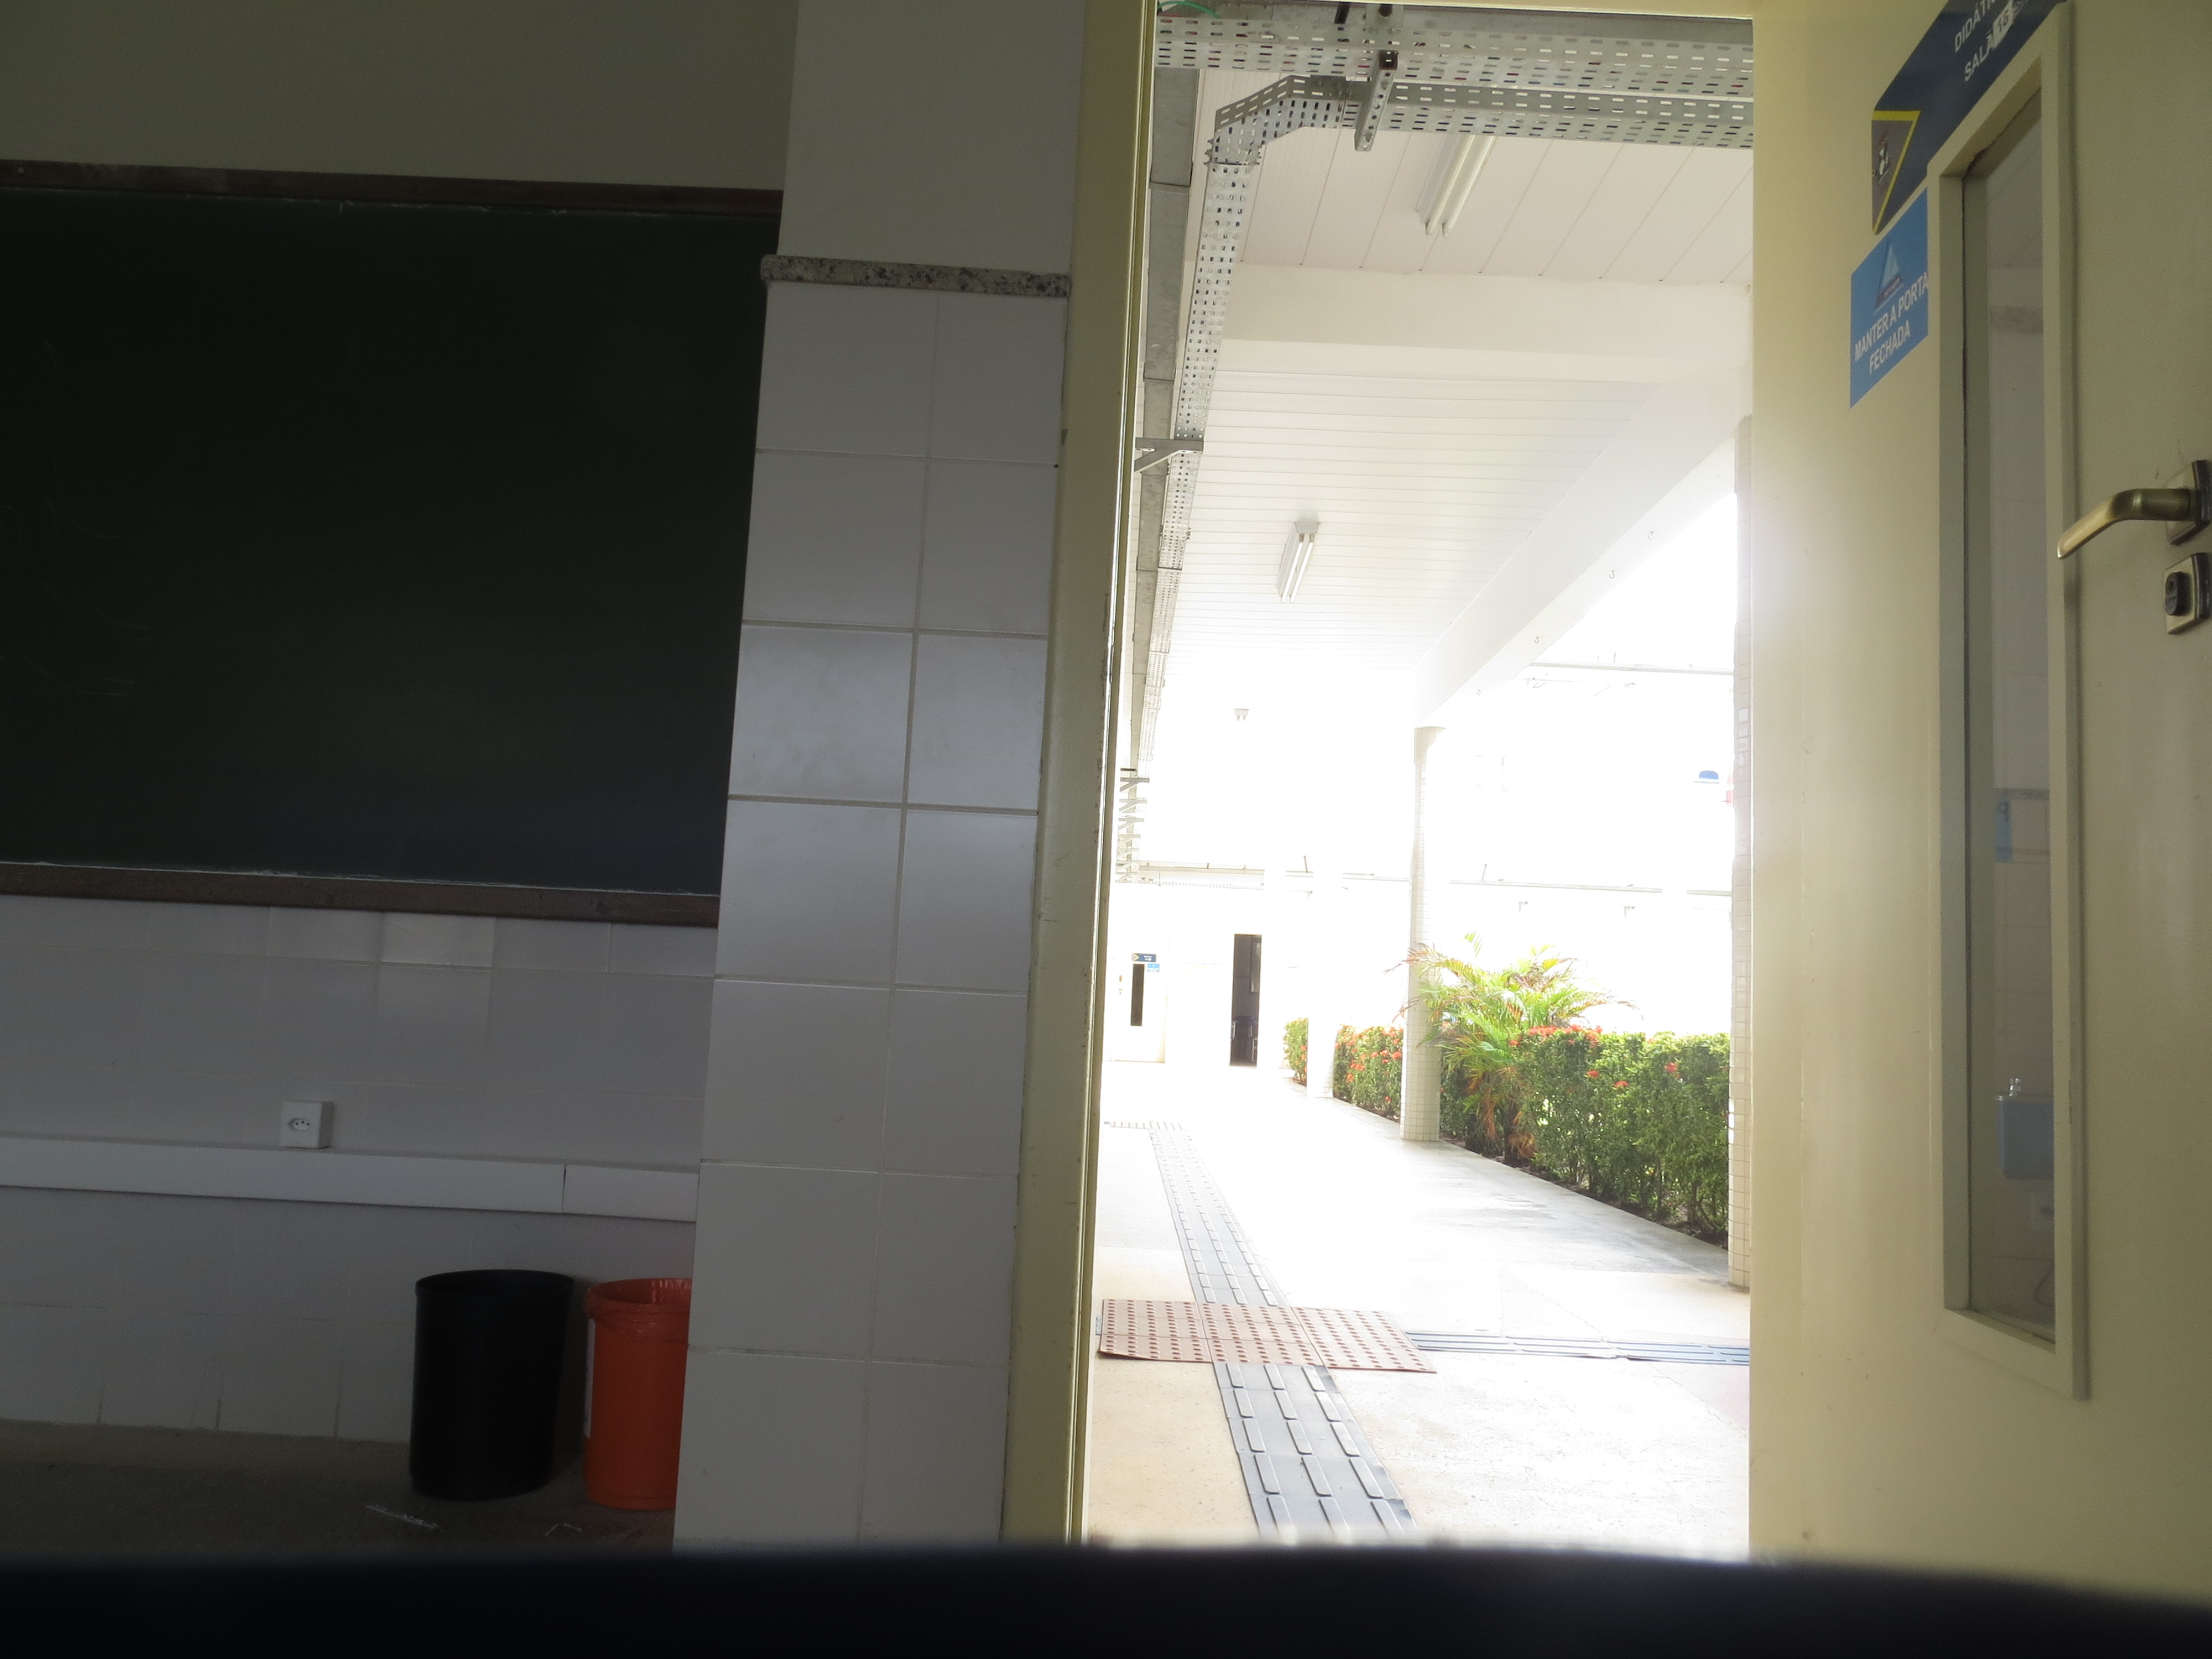
\includegraphics[height=4cm]{CenaDidatica/4}
    \label{figBaseDidaticas4}
  }
  \quad %espaco separador
  \subfloat[Tempo de exposição de $0.067s$.]
  {
    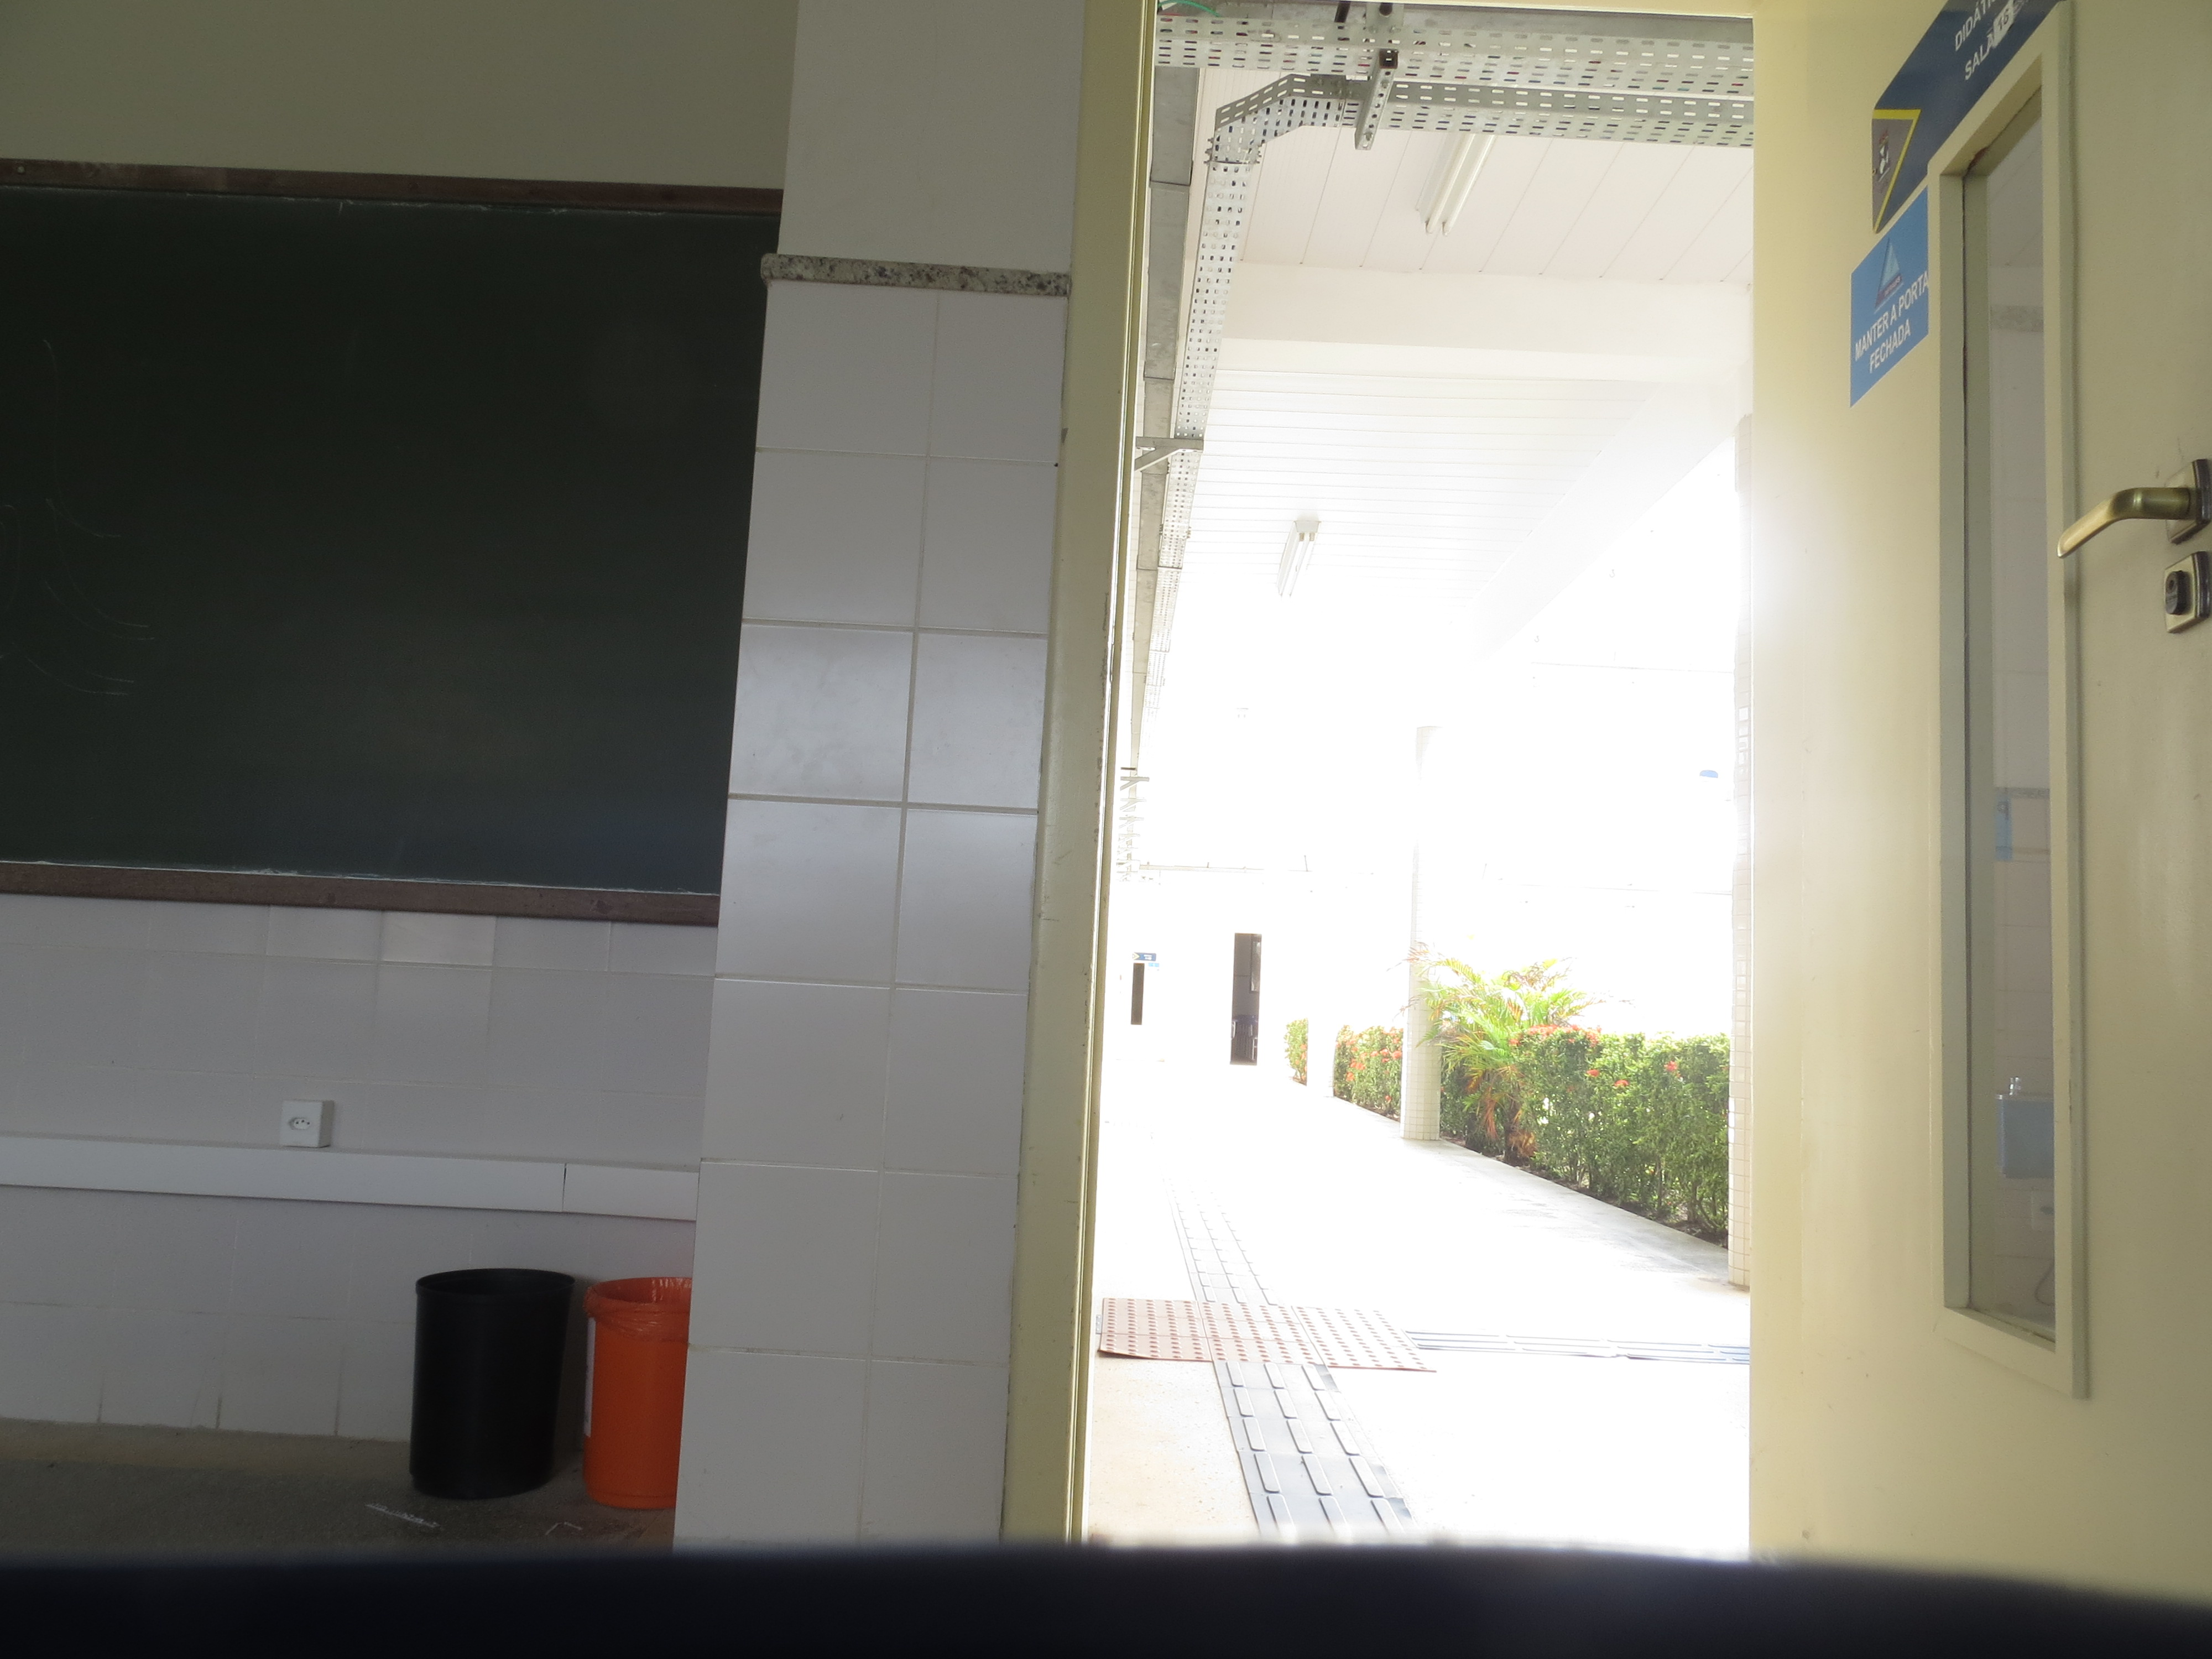
\includegraphics[height=5cm]{CenaDidatica/5}
    \label{figBaseDidaticas5}
  }
  \caption{A parte interna da sala possui baixa iluminação e é perdida nas imagens com menor tempo de exposição. A parte externa possui alta iluminação e é perdida nas imagens com maior tempo de exposição.}
  \label{figBaseDidaticas}
\end{figure}

\subsubsection{Cena da Sala de Estar} \label{cenaPorquinho}


\begin{figure}[H]
  \subfloat[Tempo de exposição de $0.077s$.]
  {
    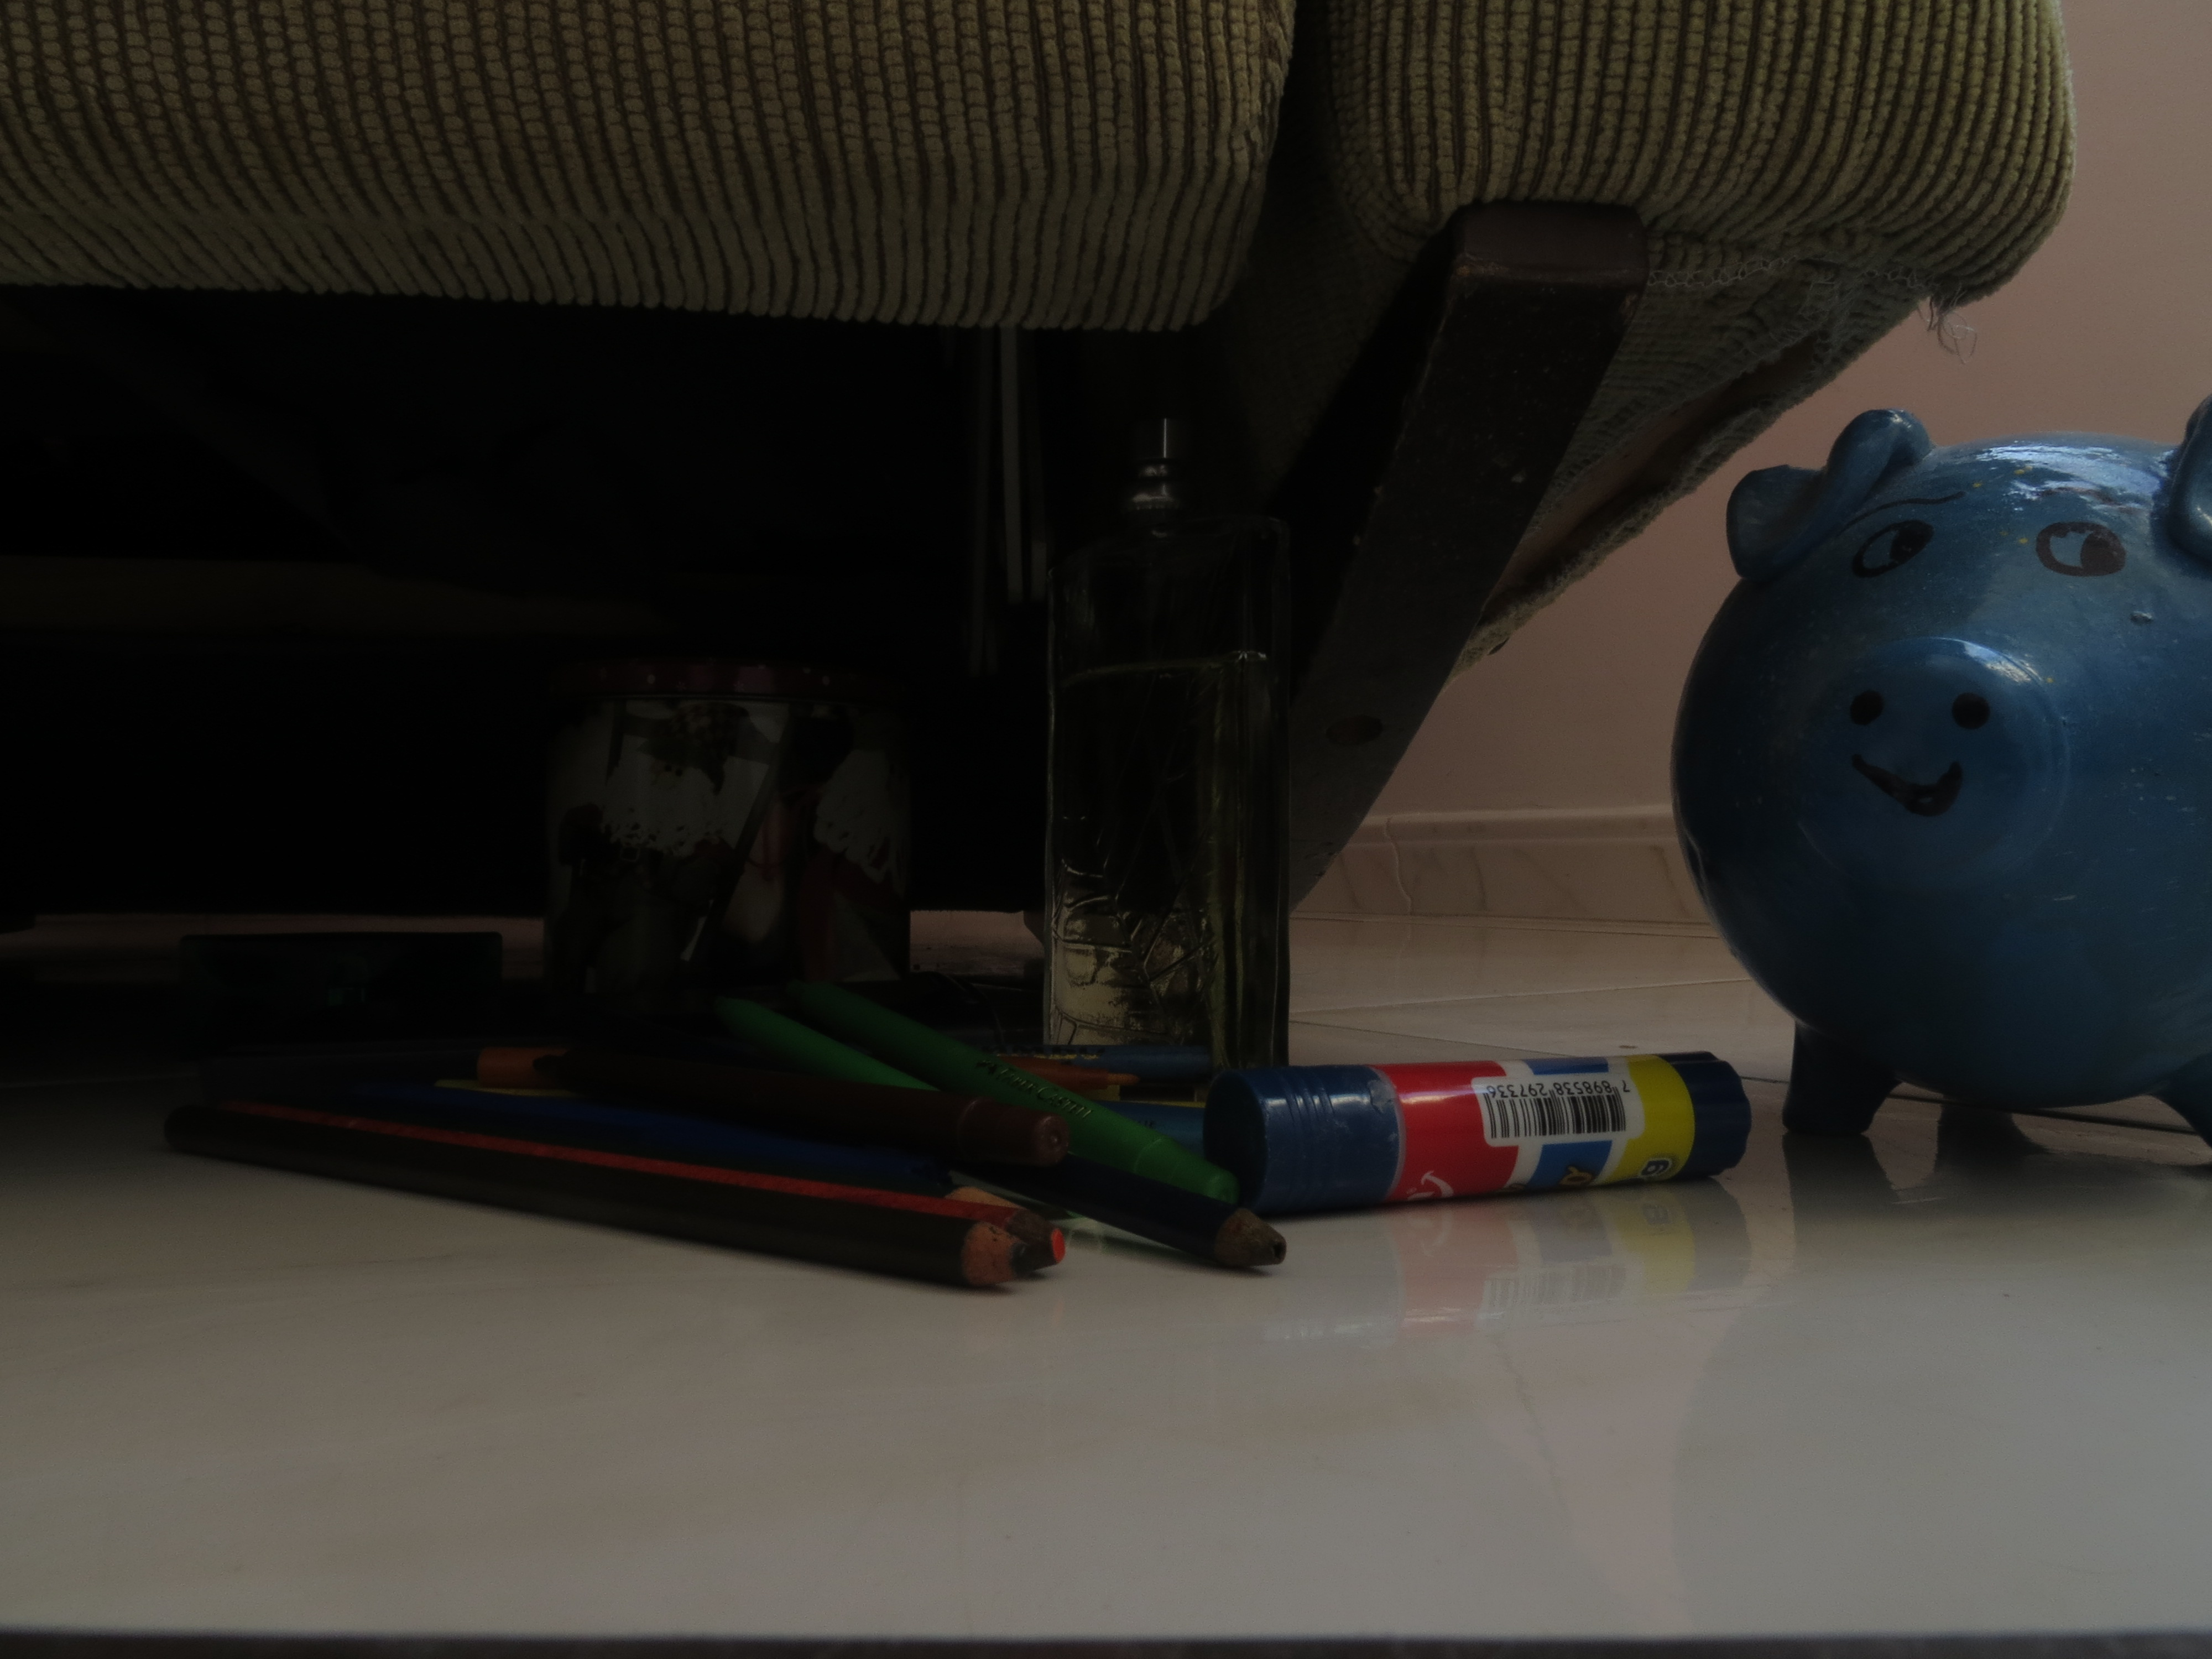
\includegraphics[height=5cm]{CenaPorquinho/1}
    \label{figBasePorquinho1}
  }
  \quad %espaco separador
  \subfloat[Tempo de exposição de $0.25s$.]
  {
    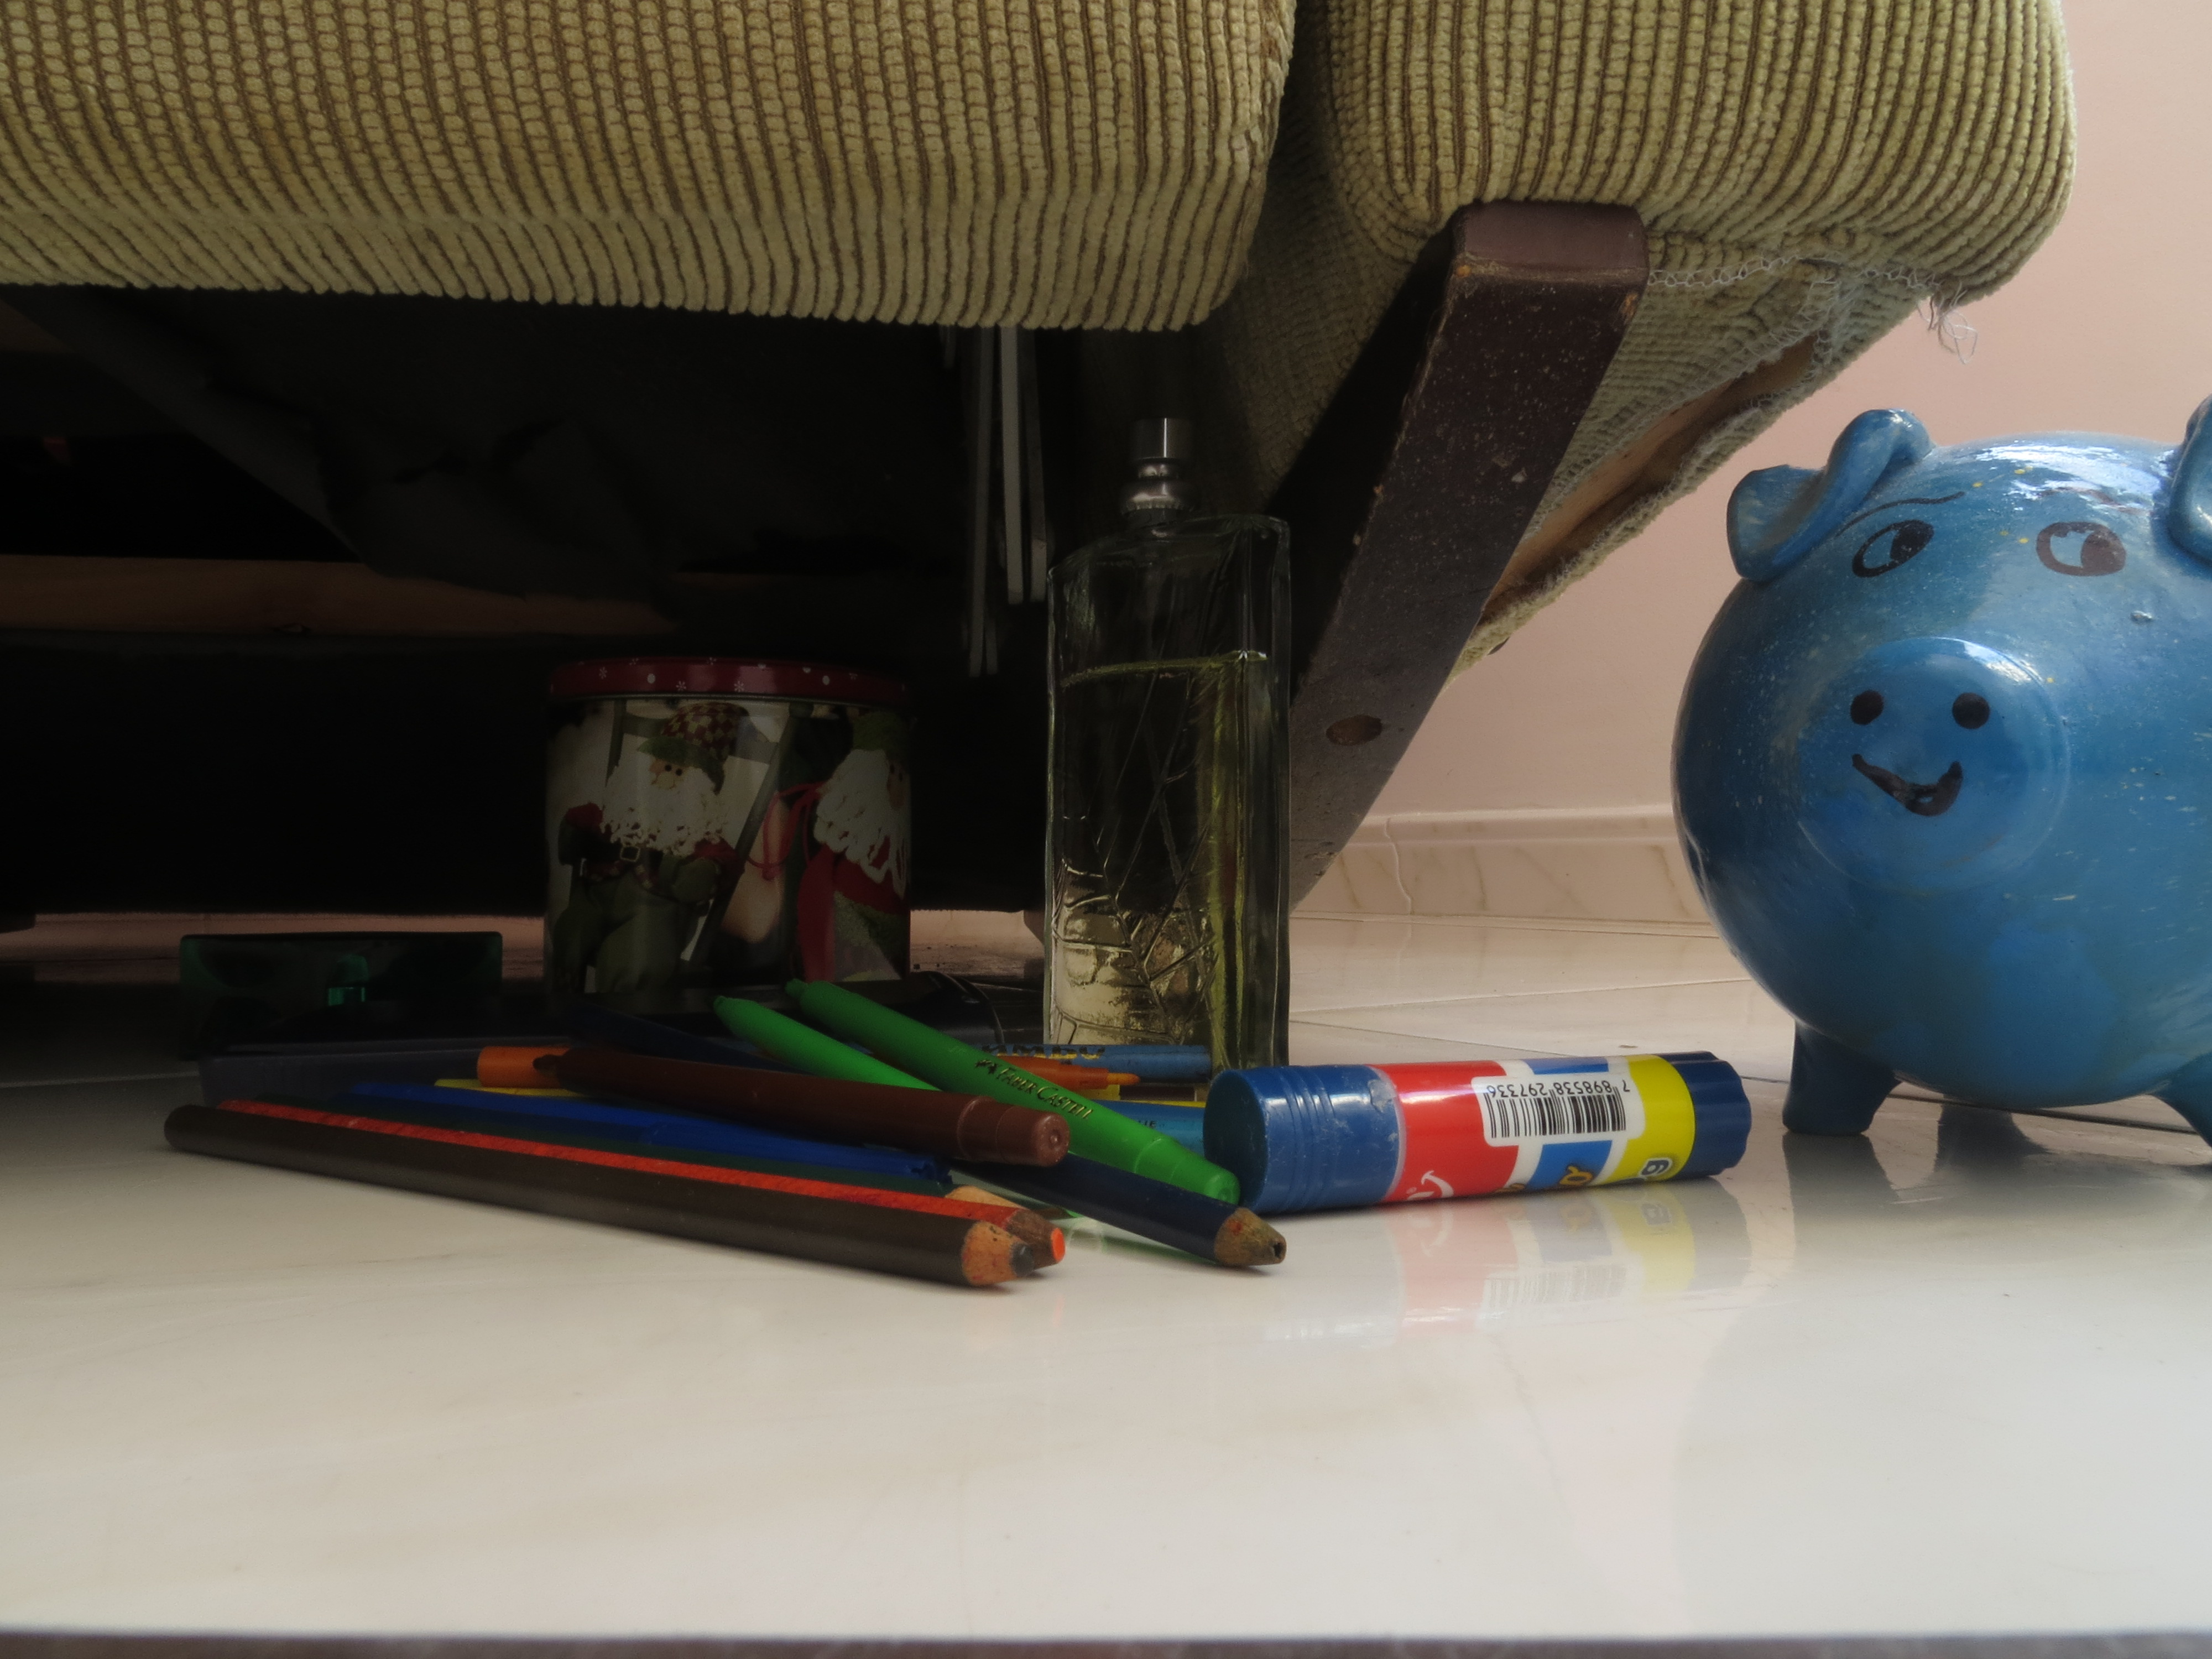
\includegraphics[height=5cm]{CenaPorquinho/2}
    \label{figBasePorquinho2}
  }
  \quad %espaco separador
  \subfloat[Tempo de exposição de $0.6s$.]
  {
    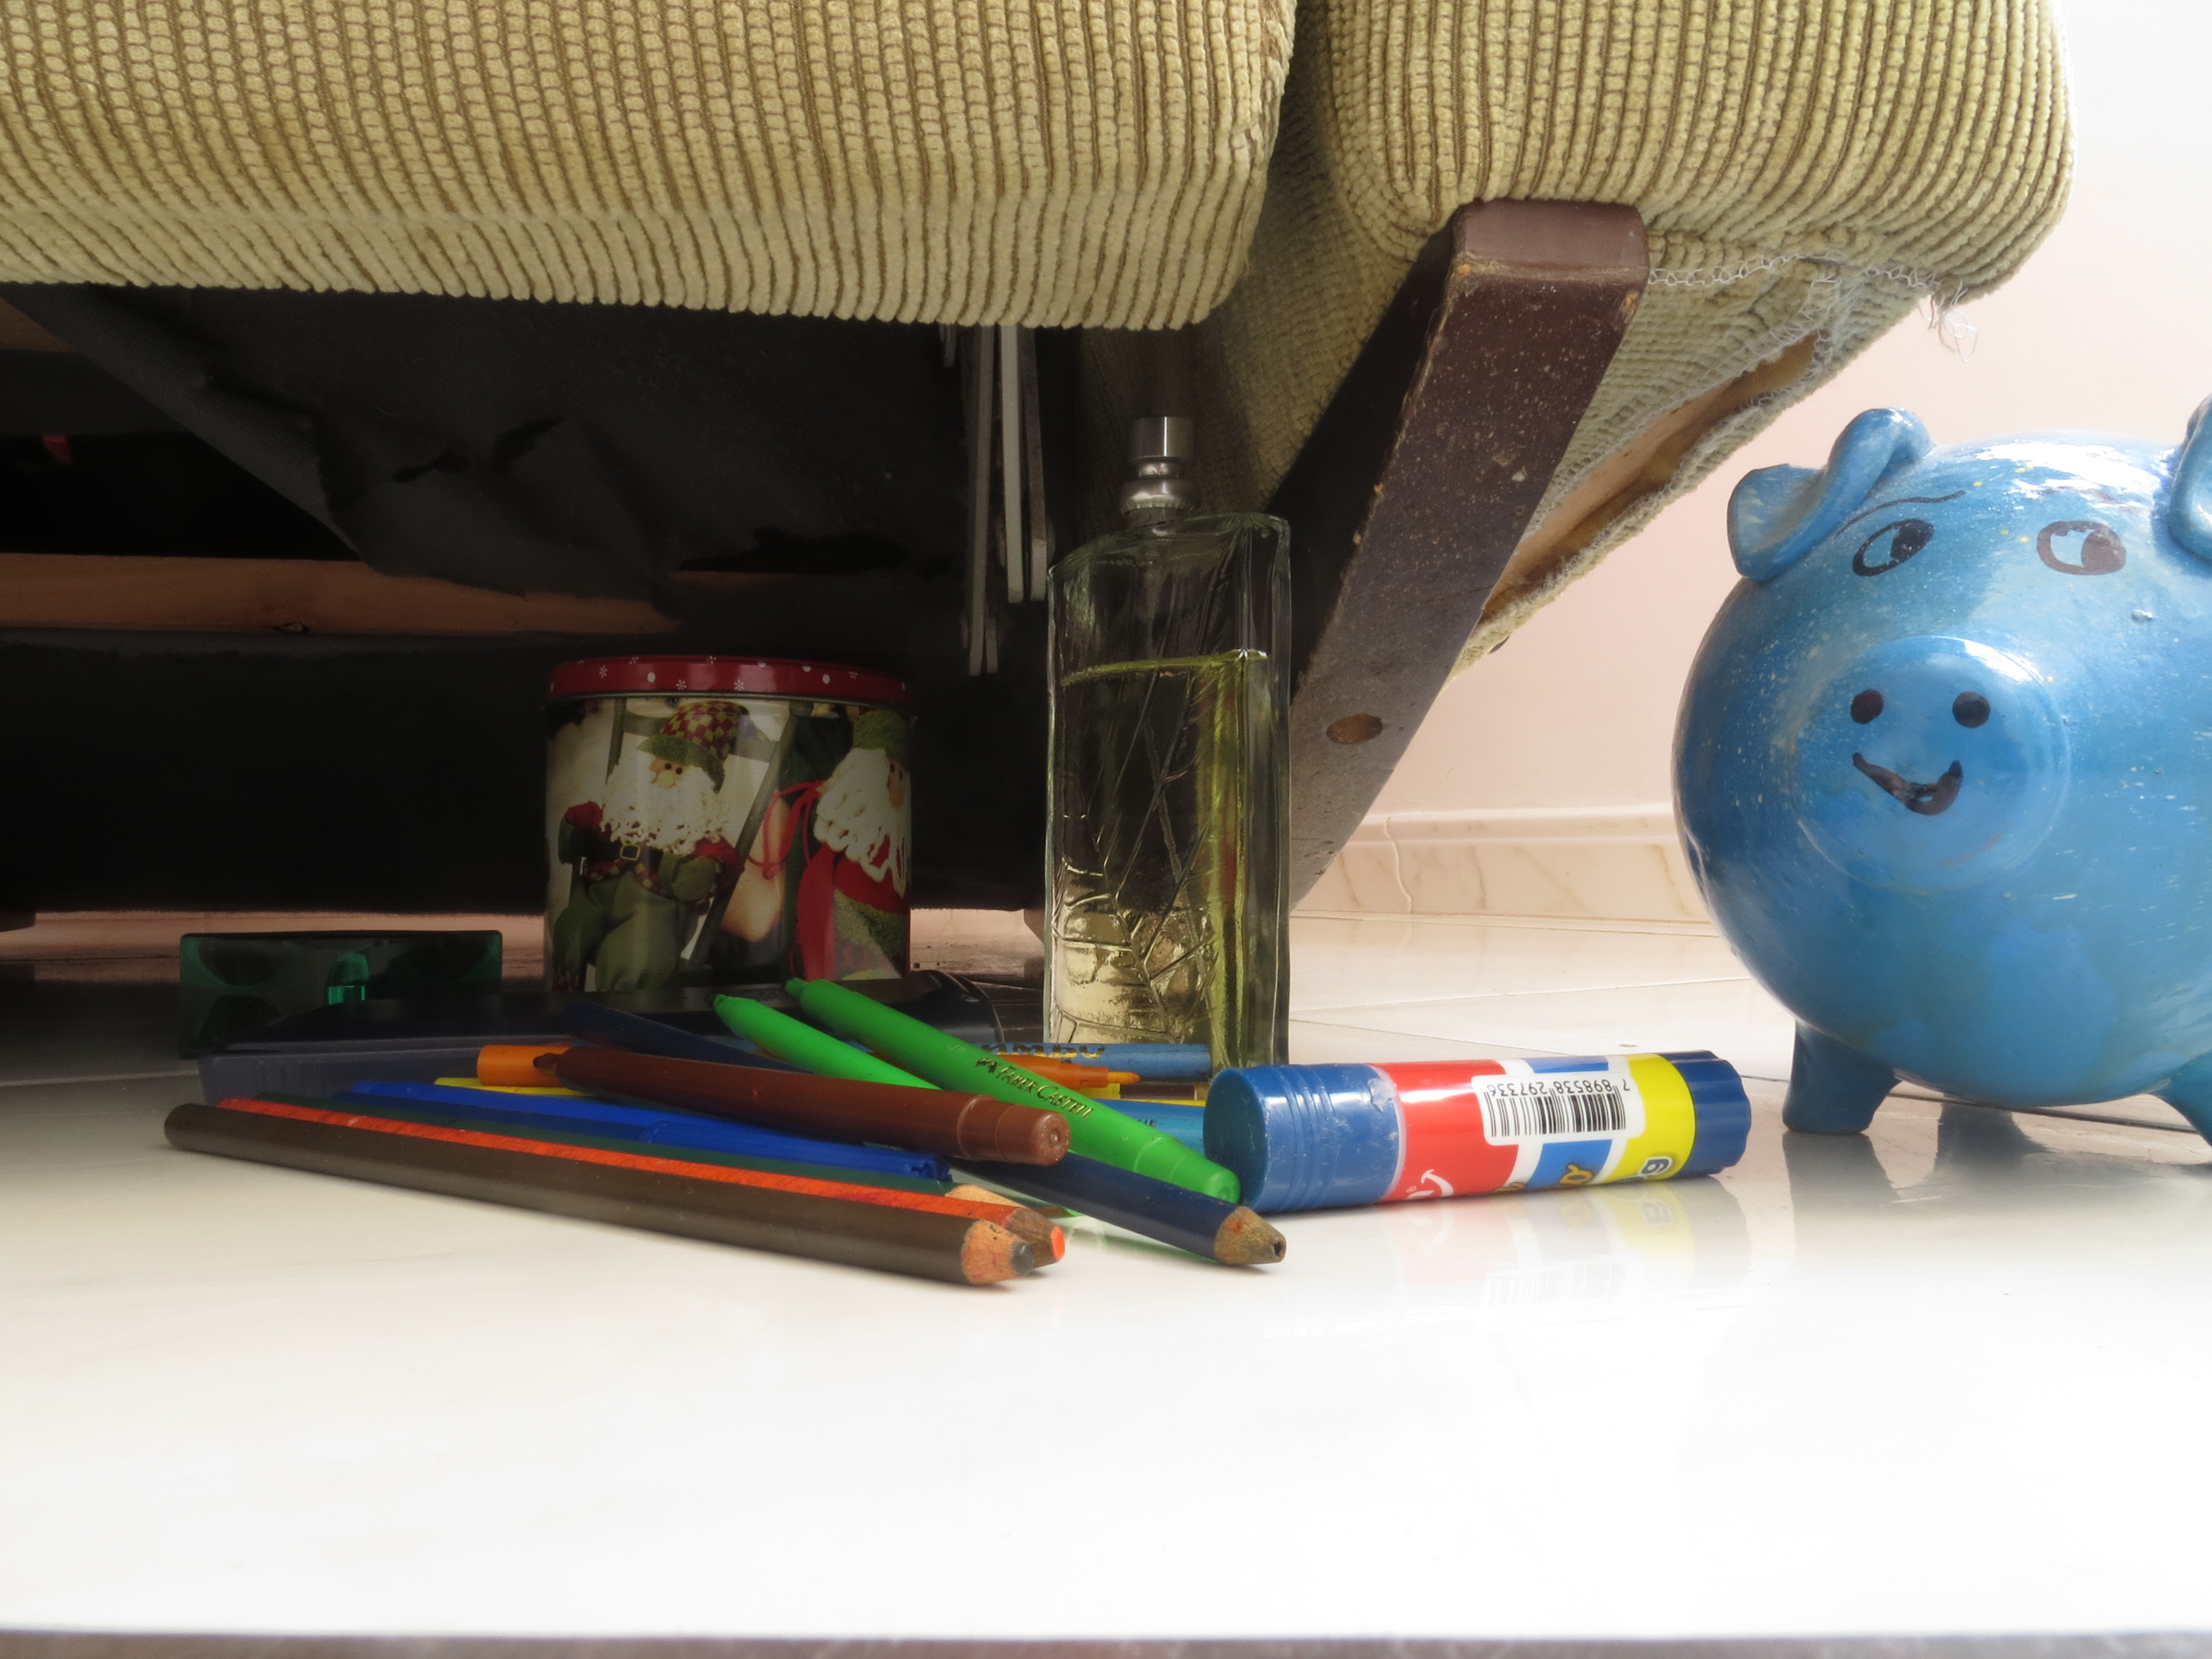
\includegraphics[height=5cm]{CenaPorquinho/3}
    \label{figBasePorquinho3}
  }
  \quad %espaco separador
  \subfloat[Tempo de exposição de $1.3s$.]
  {
    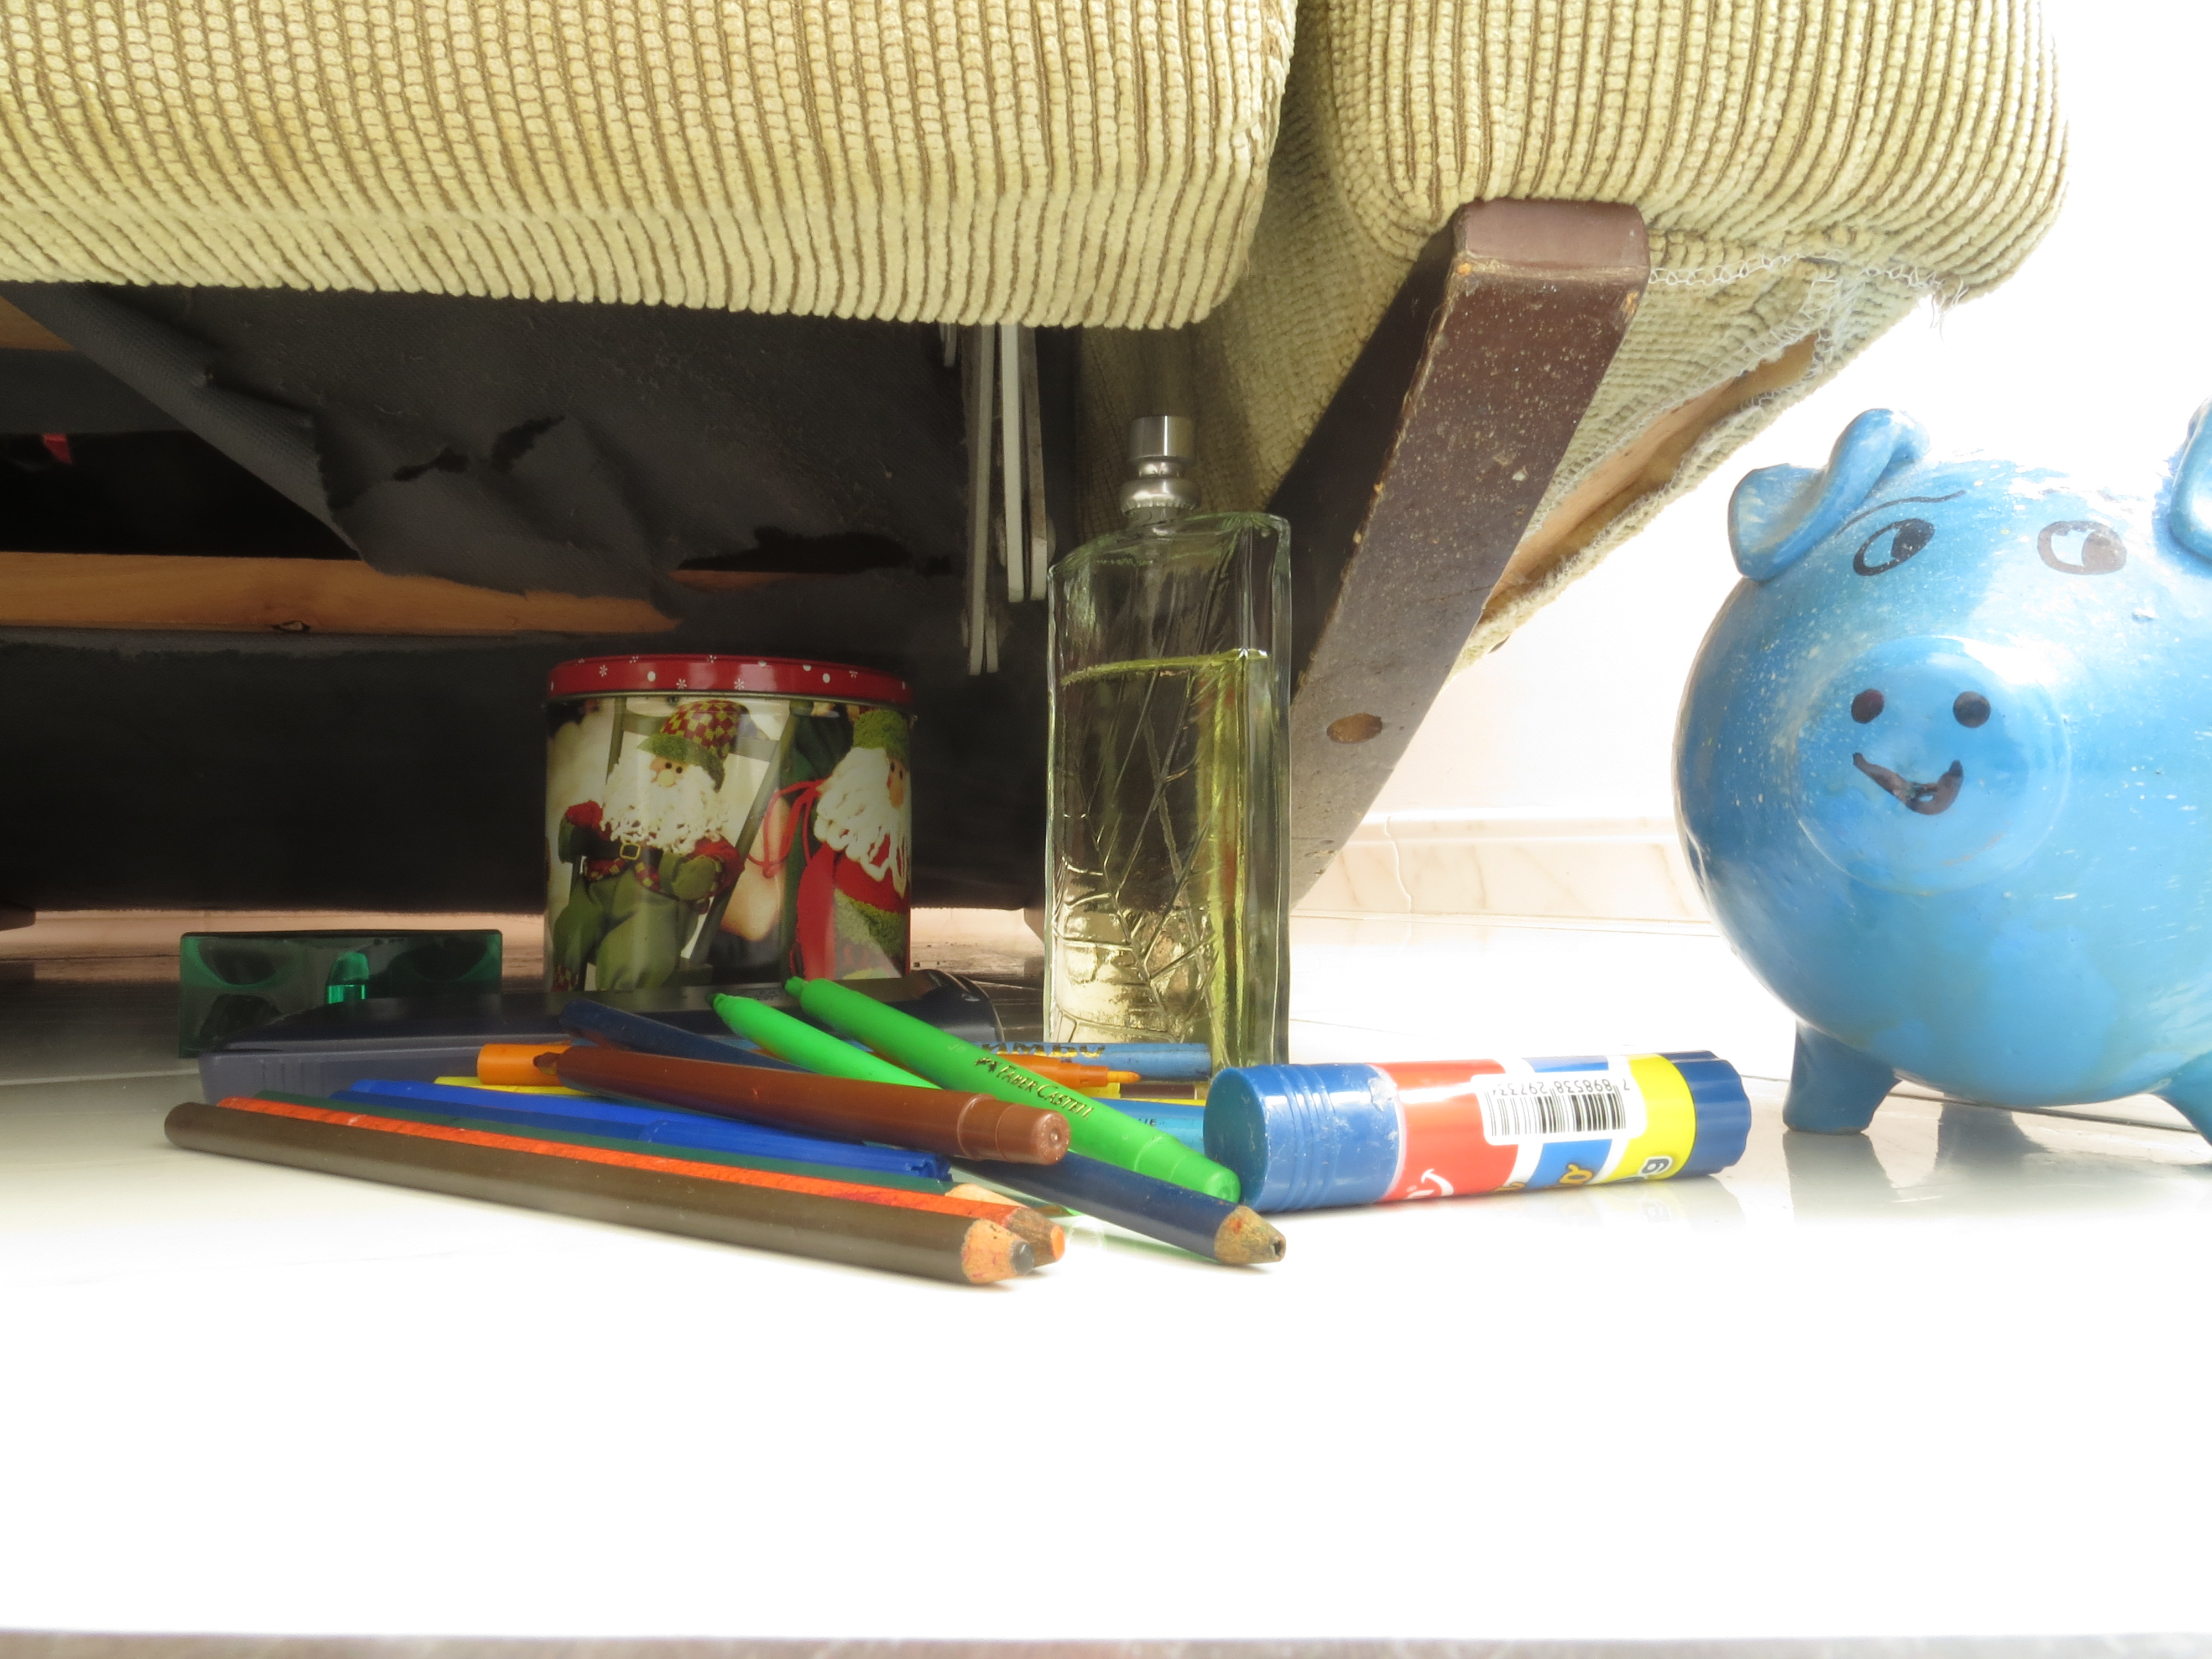
\includegraphics[height=5cm]{CenaPorquinho/4}
    \label{figBasePorquinho4}
  }
  \caption{Partes da cena são perdidas em algumas figuras. Porém estas mesmas partes estão bem representadas em outras.}
  \label{figBasePorquinho}
\end{figure}


\subsubsection{Cena dos Livros} \label{cenaOlhinhos}

\begin{figure}[H]
  \subfloat[Tempo de exposição de $0.02s$.]
  {
    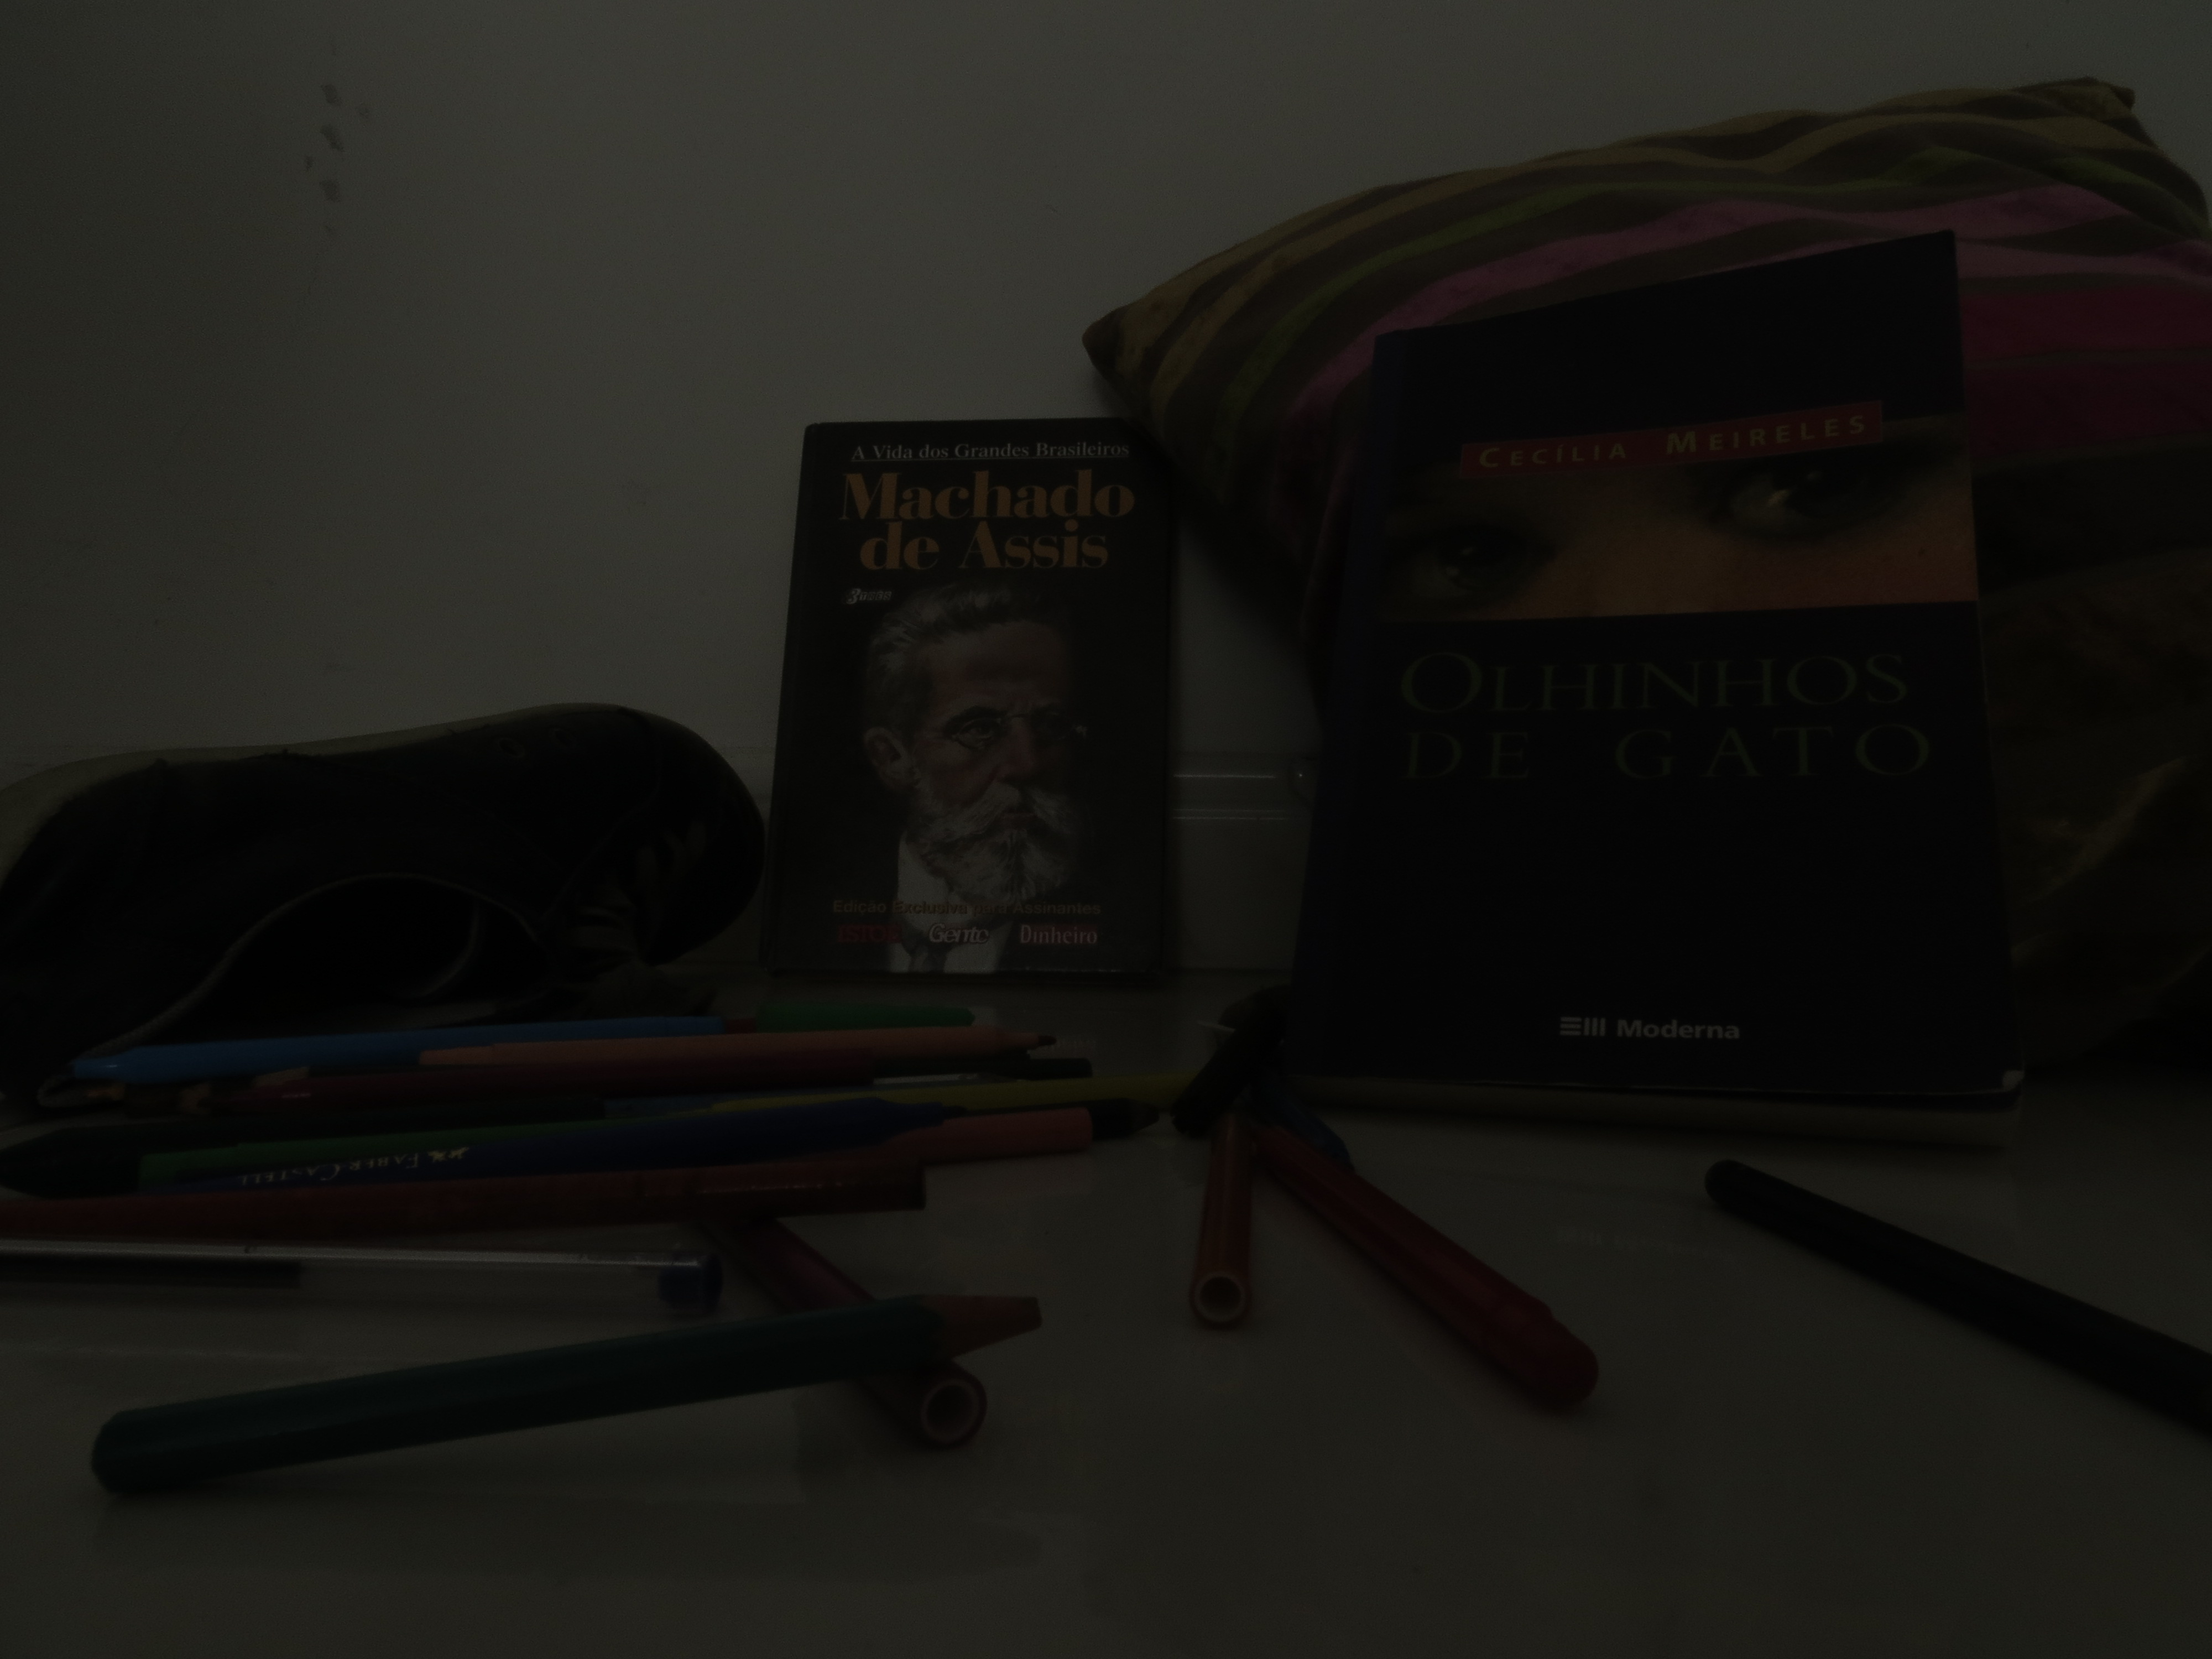
\includegraphics[height=5cm]{CenaOlhinhos/1}
    \label{figBaseOlhihos1}
  }
  \quad %espaco separador
  \subfloat[Tempo de exposição de $0.067s$.]
  {
    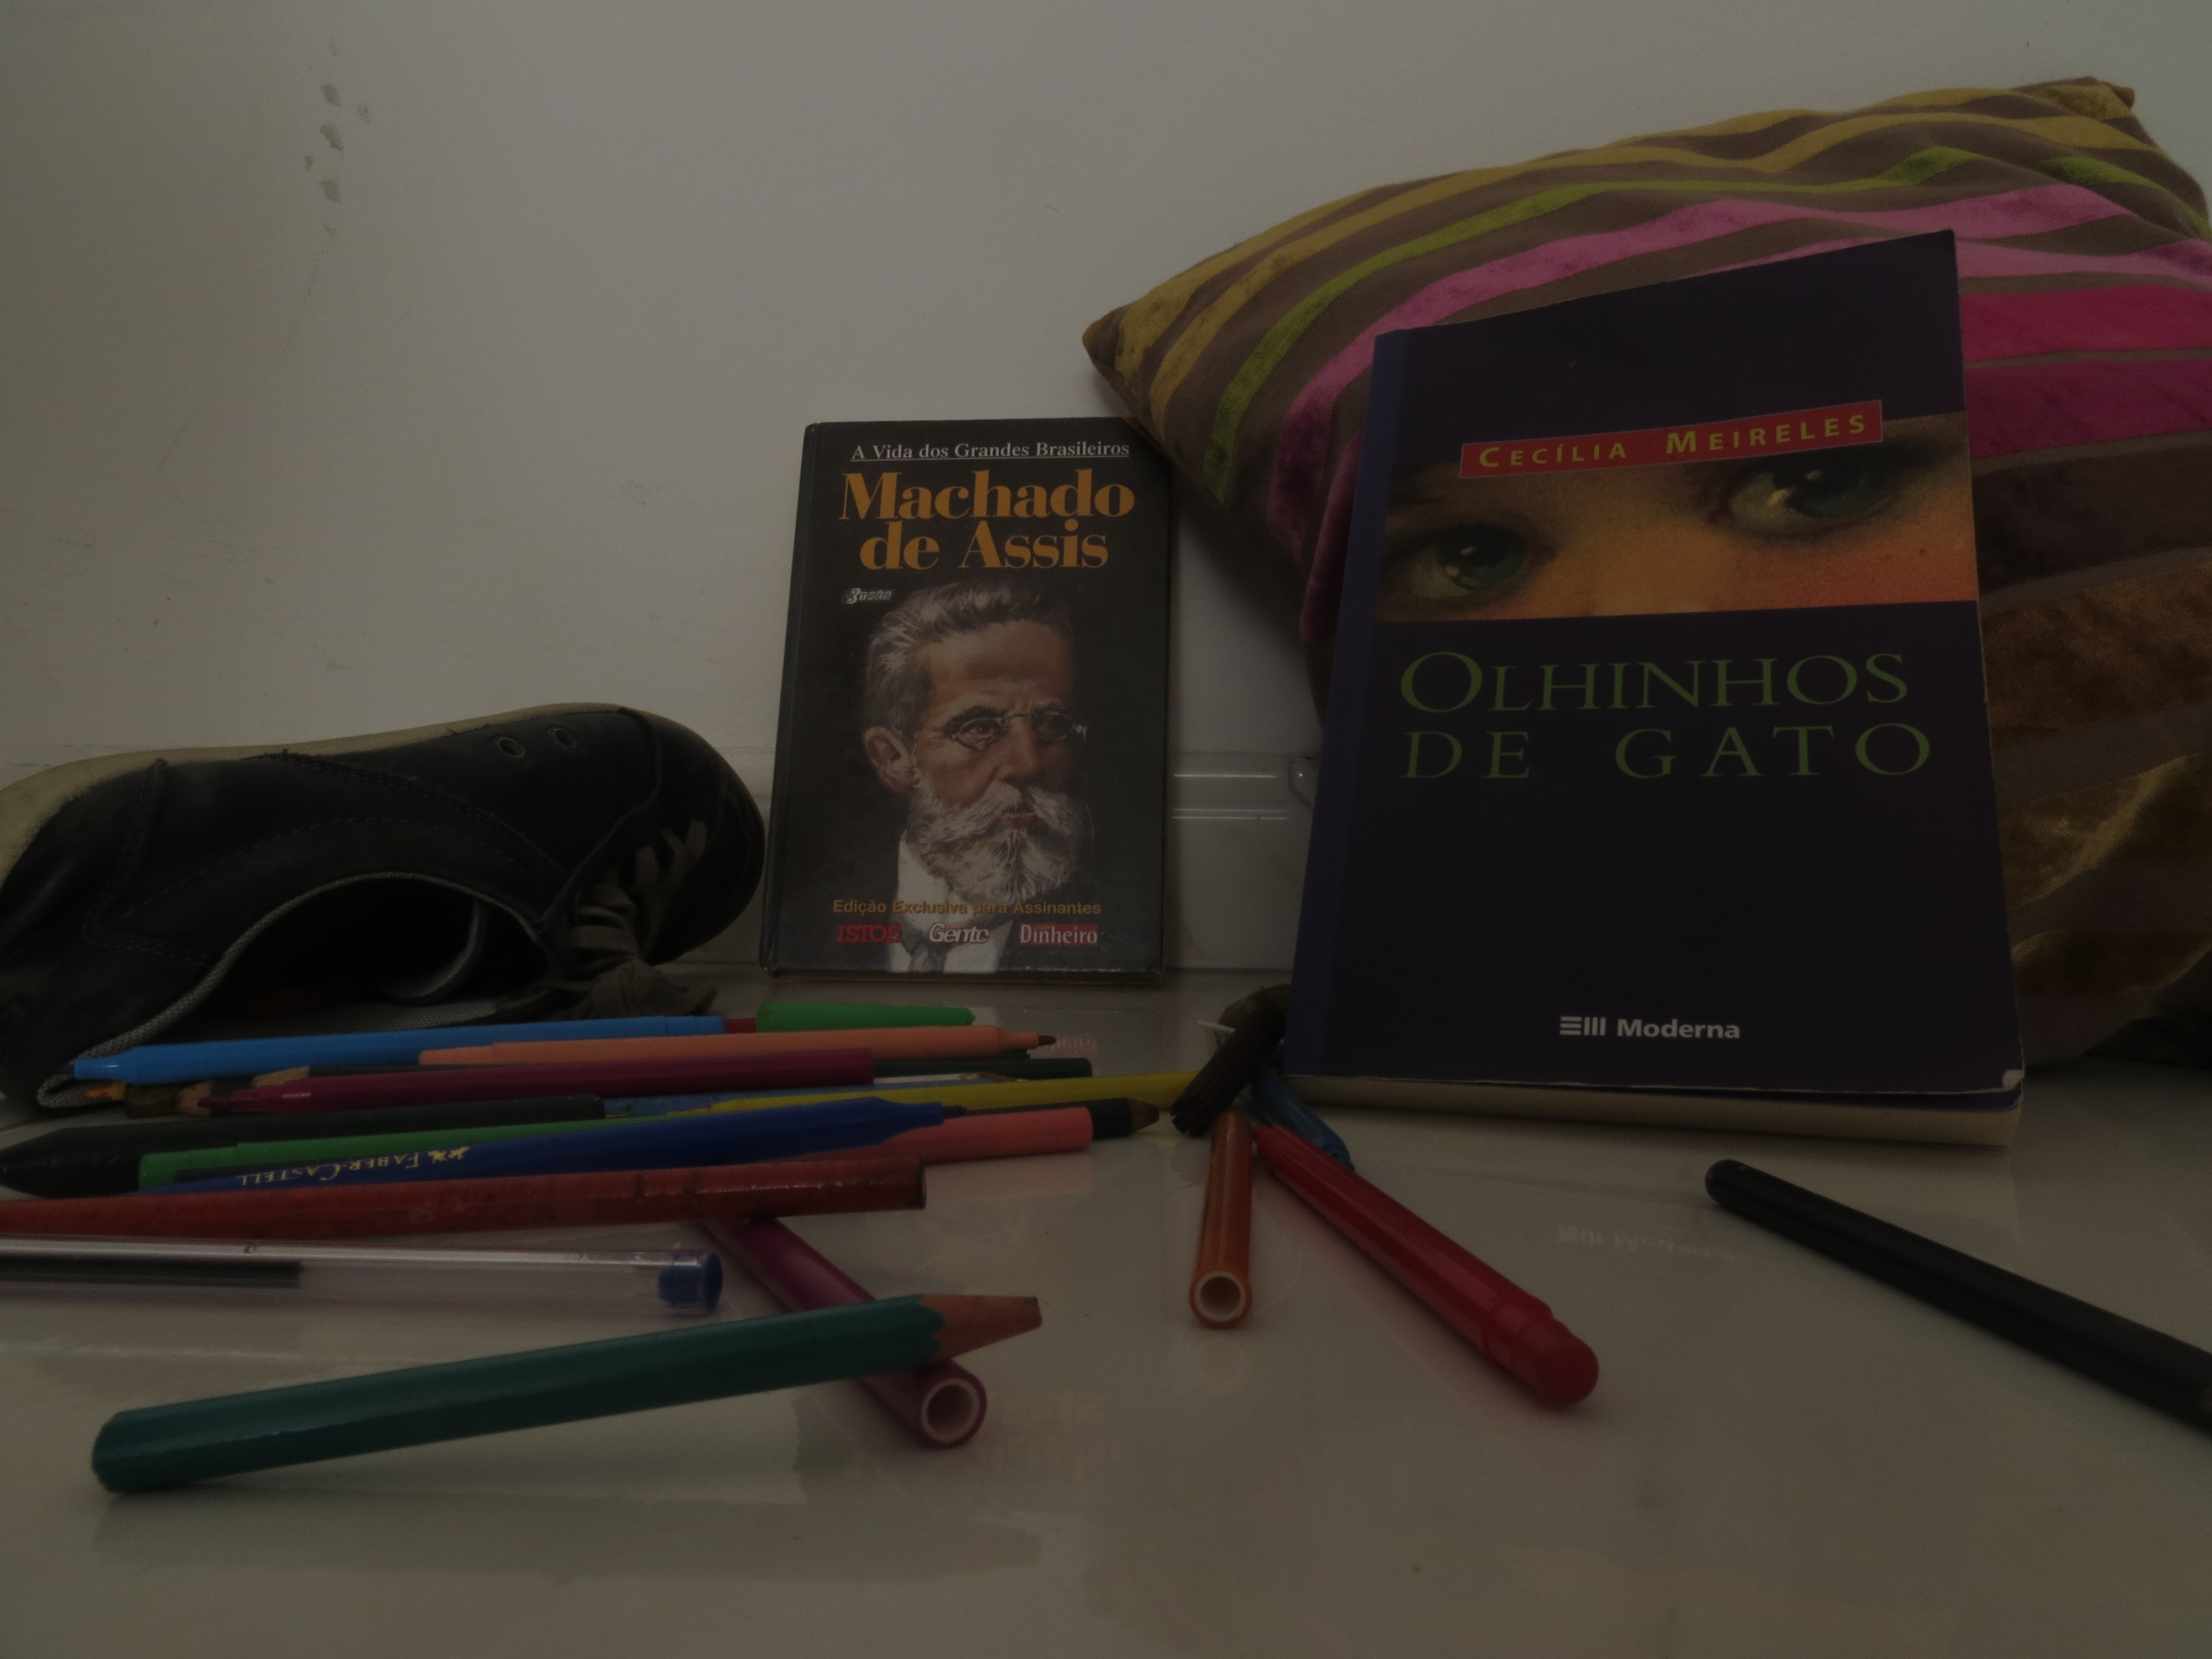
\includegraphics[height=5cm]{CenaOlhinhos/2}
    \label{figBaseOlhihos2}
  }
  \quad %espaco separador
  \subfloat[Tempo de exposição de $0.2s$.]
  {
    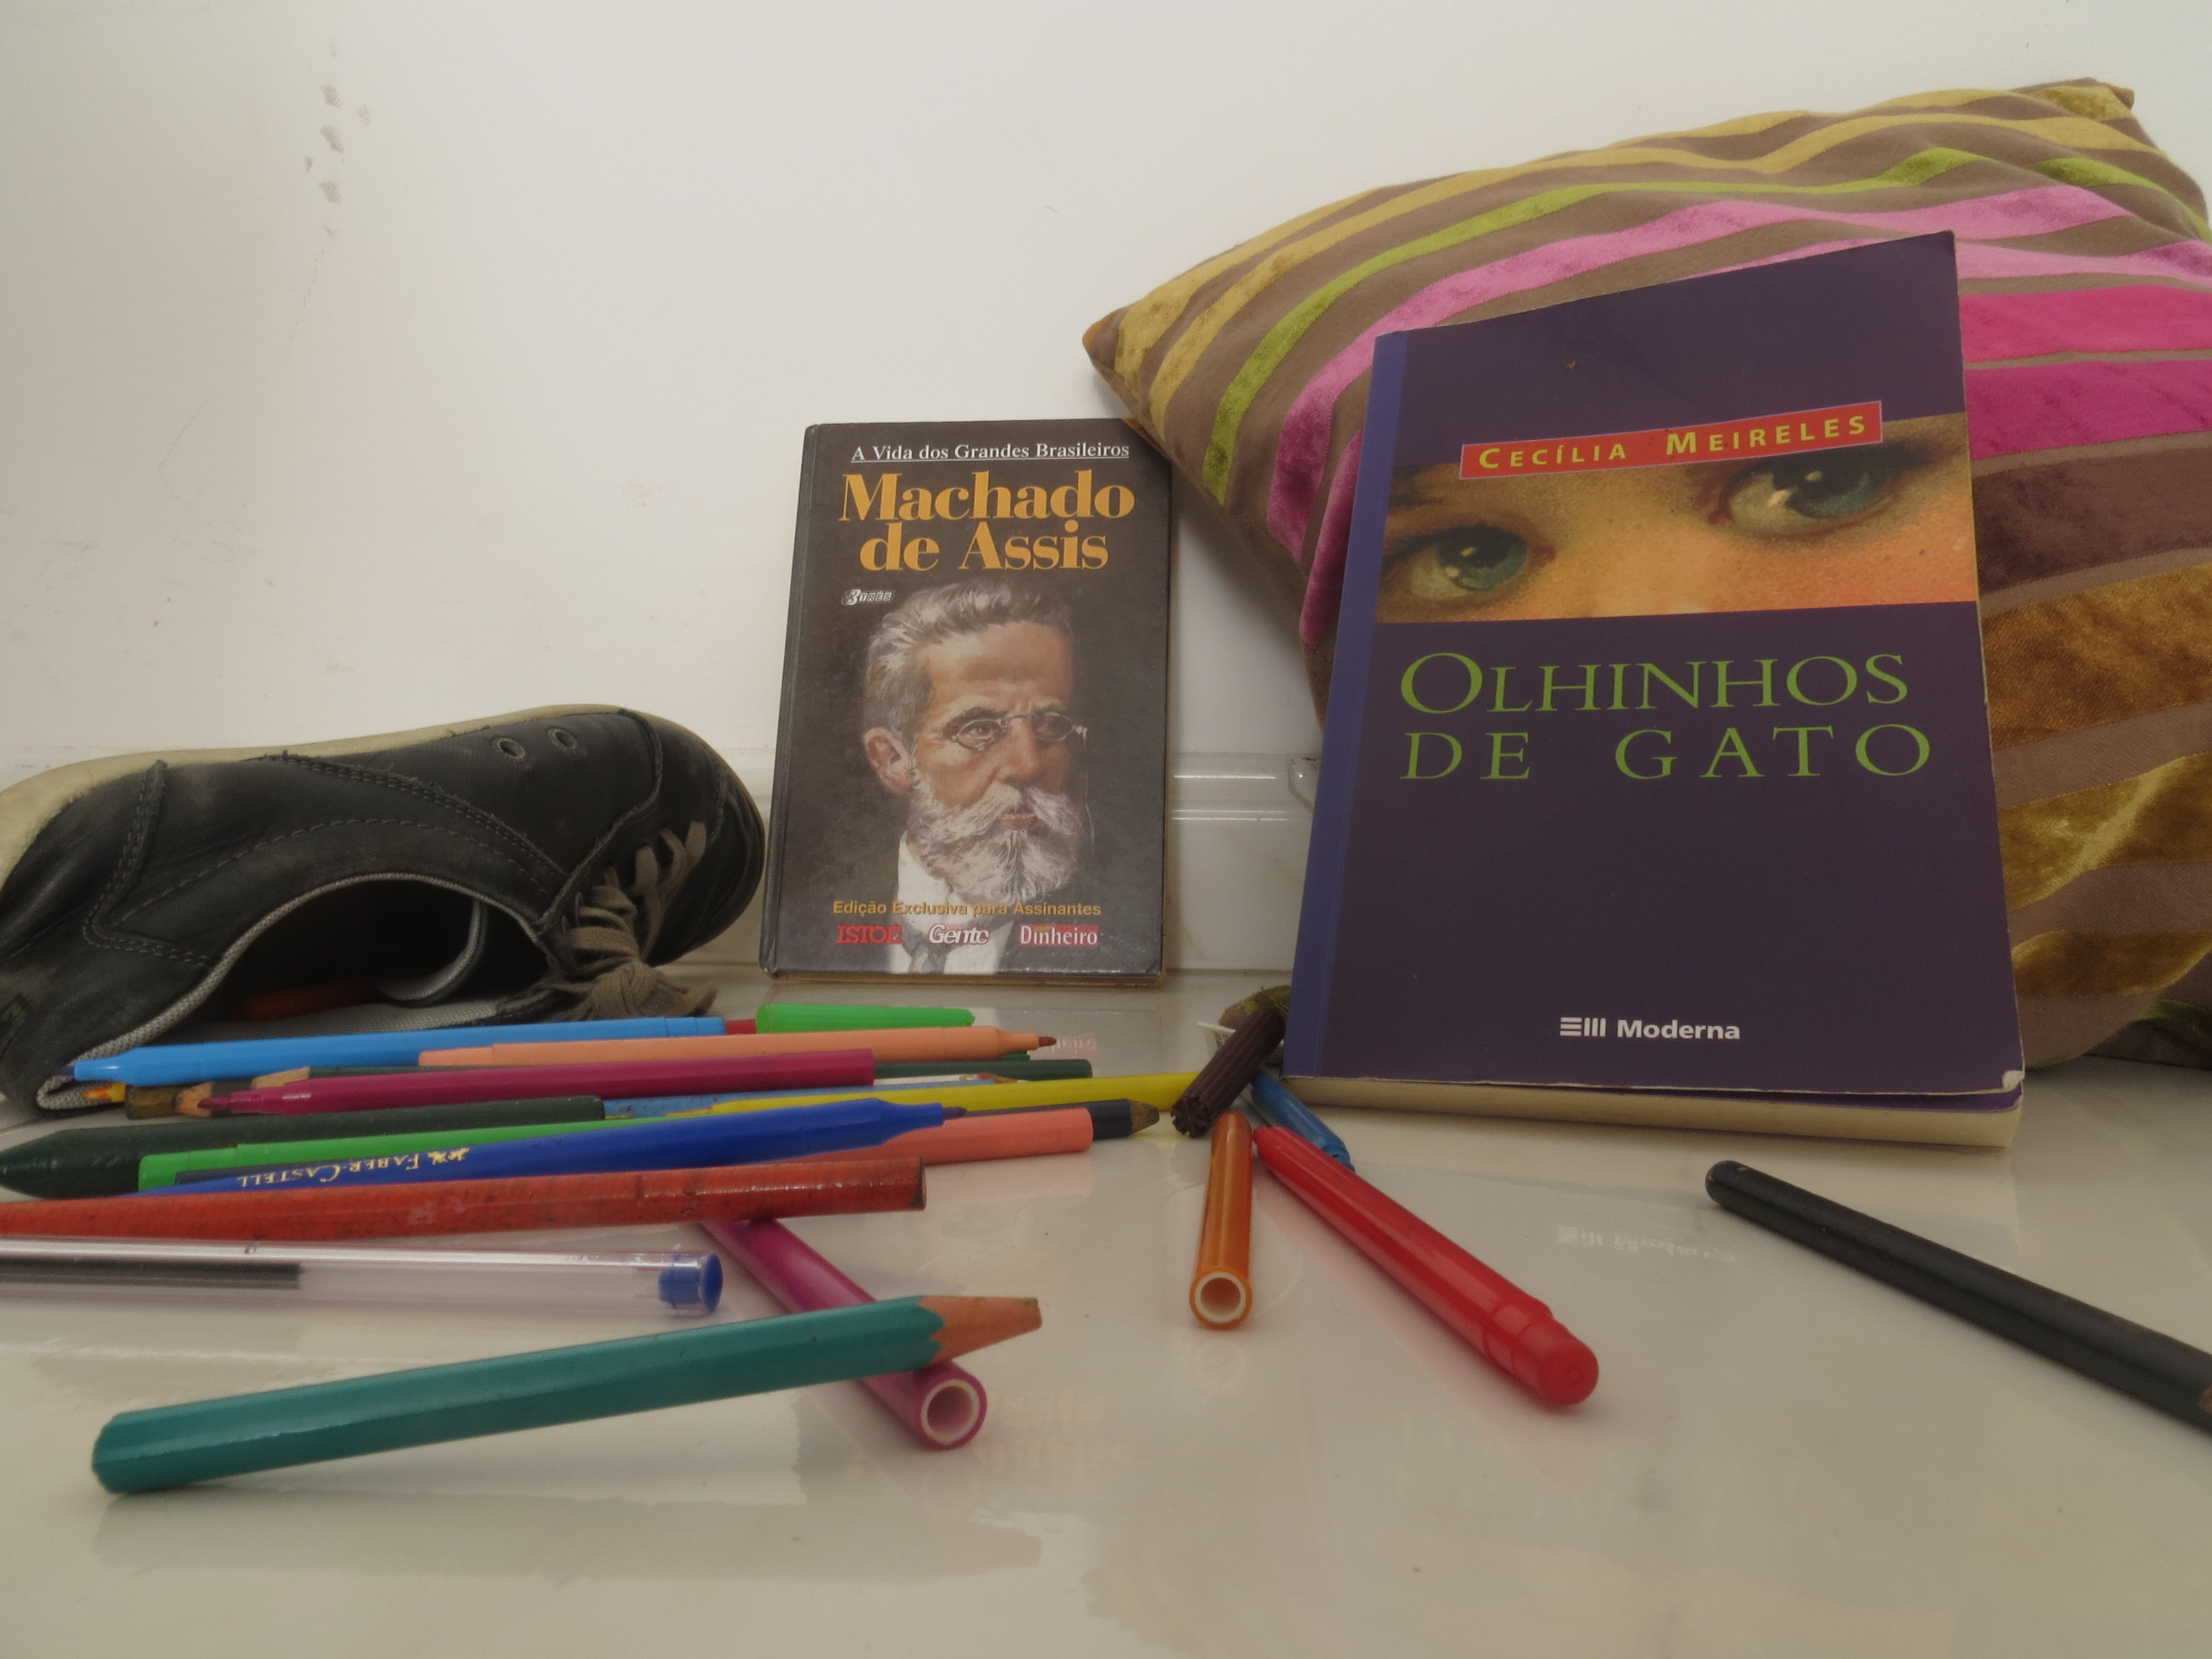
\includegraphics[height=5cm]{CenaOlhinhos/3}
    \label{figBaseOlhihos3}
  }
  \quad %espaco separador
  \subfloat[Tempo de exposição de $0.6s$.]
  {
    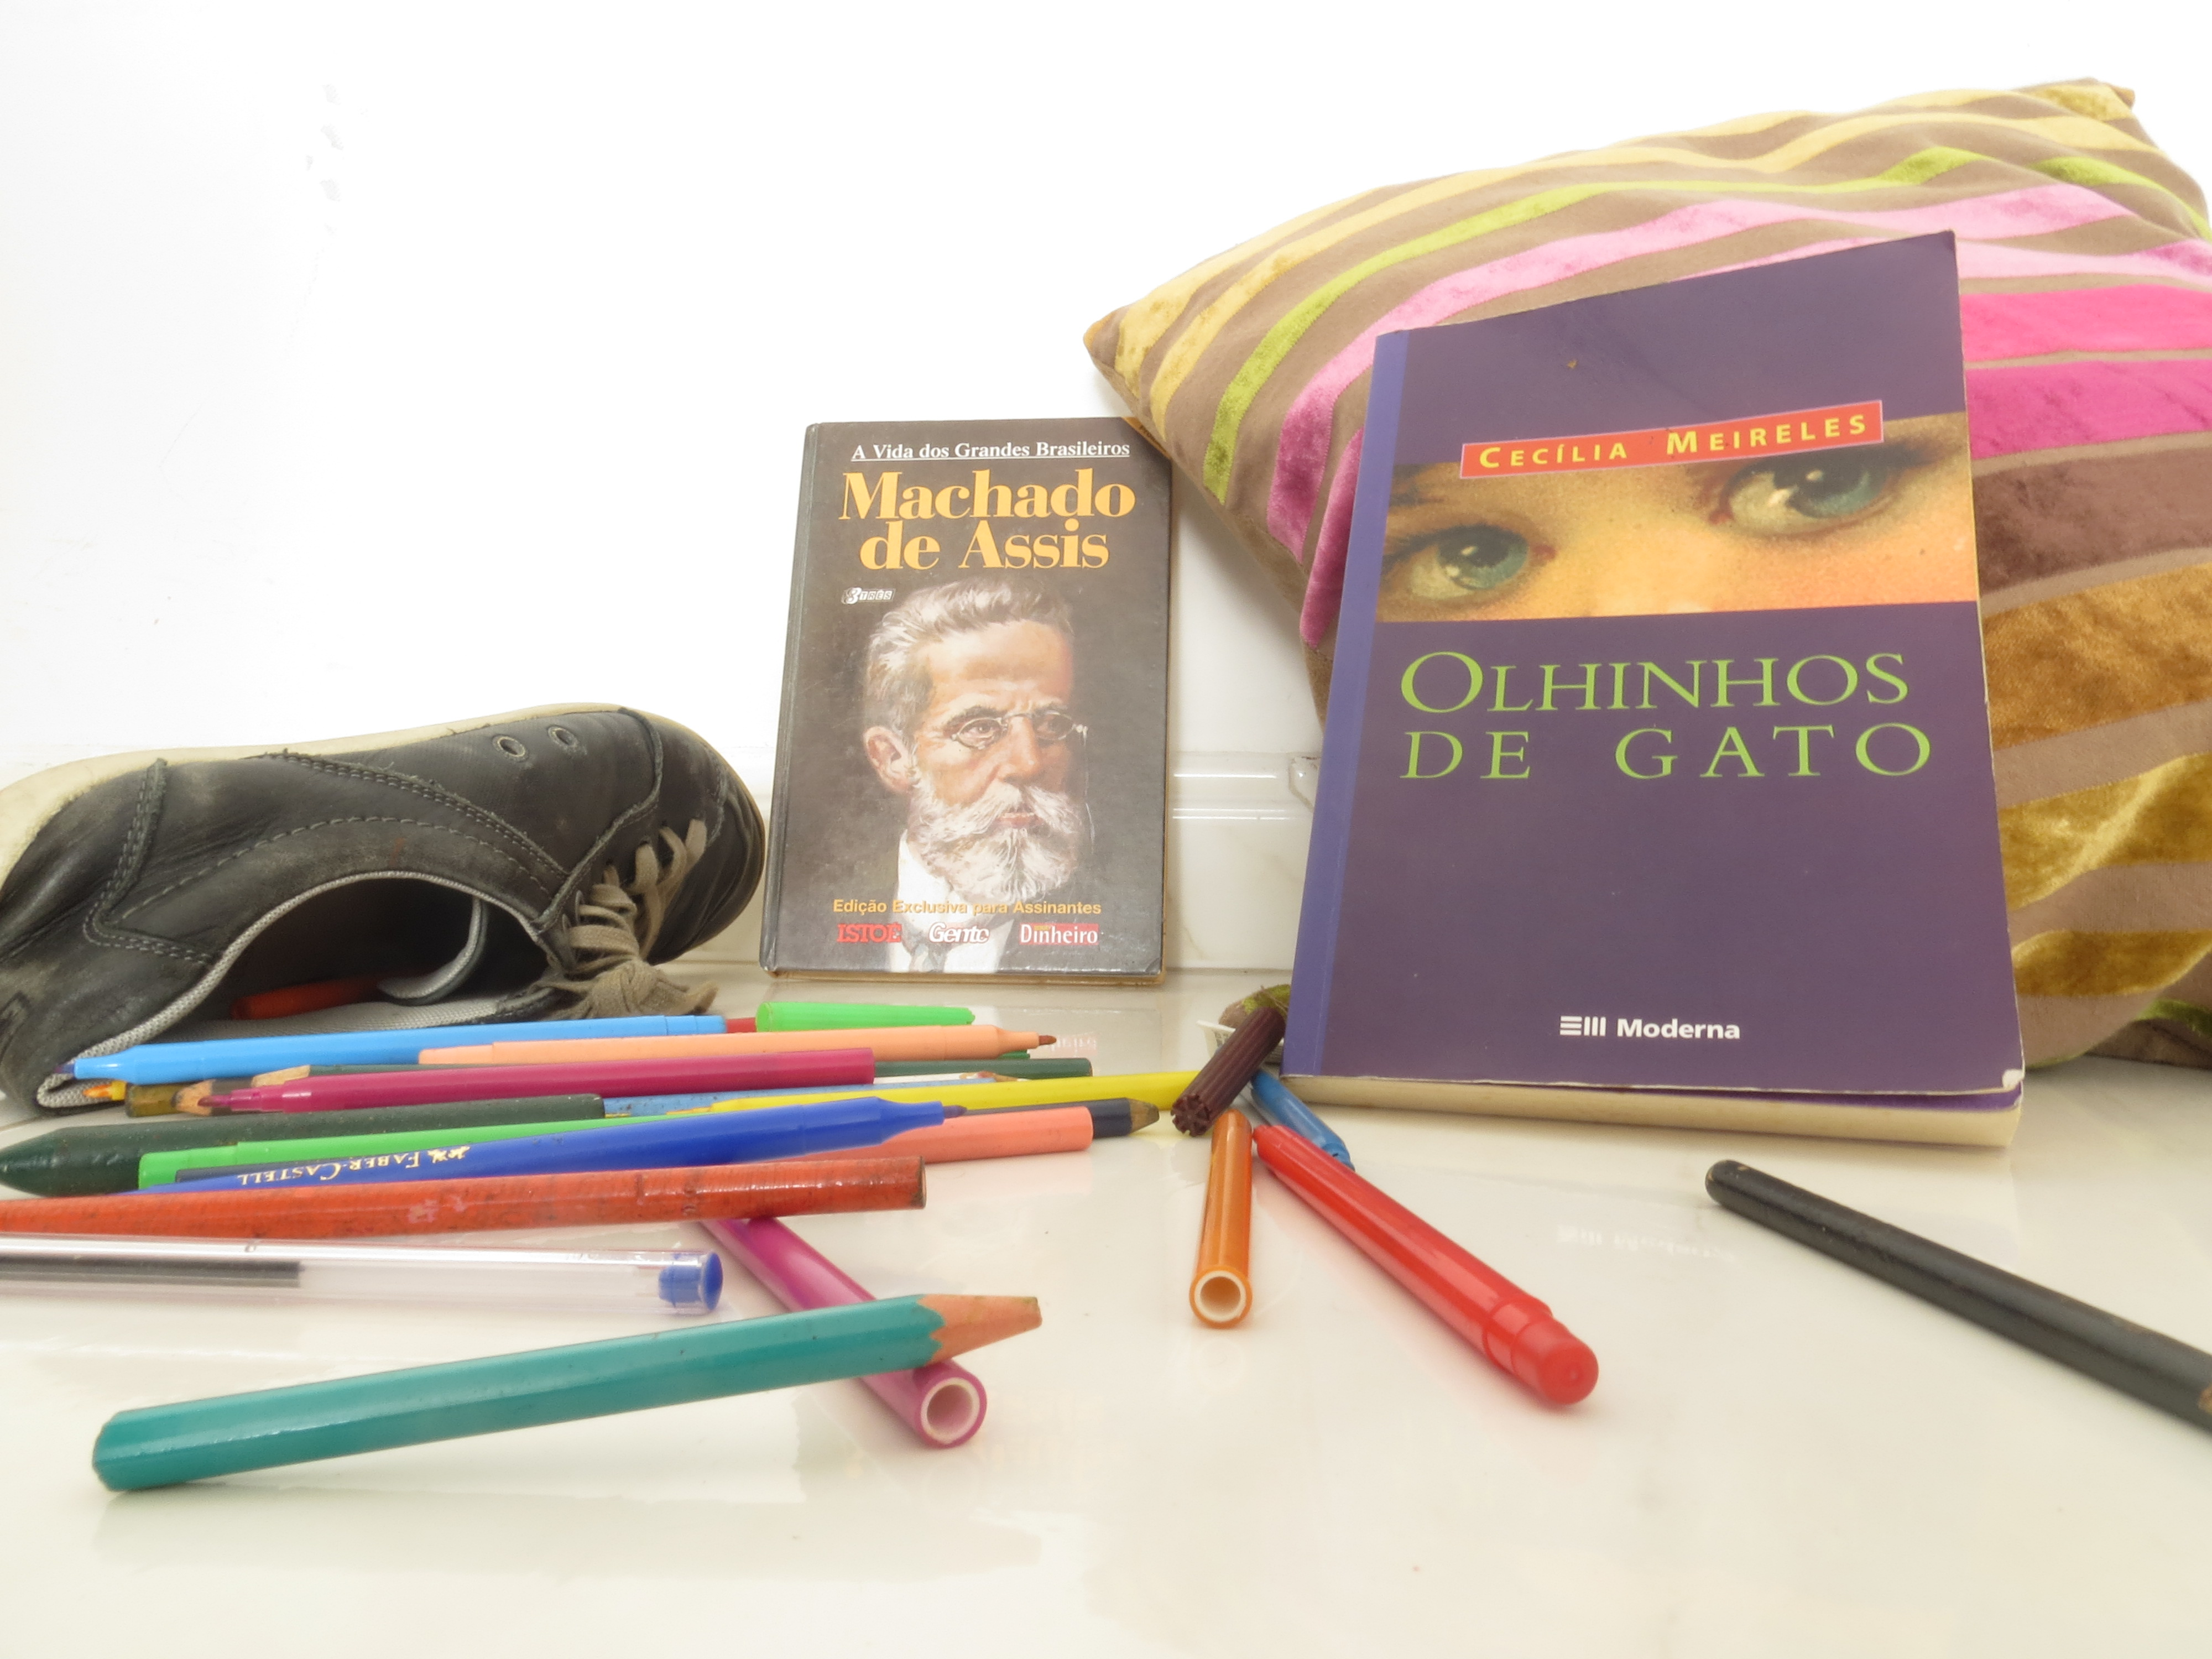
\includegraphics[height=5cm]{CenaOlhinhos/4}
    \label{figBaseOlhihos4}
  }
  \quad %espaco separador
  \subfloat[Tempo de exposição de $2.0s$.]
  {
    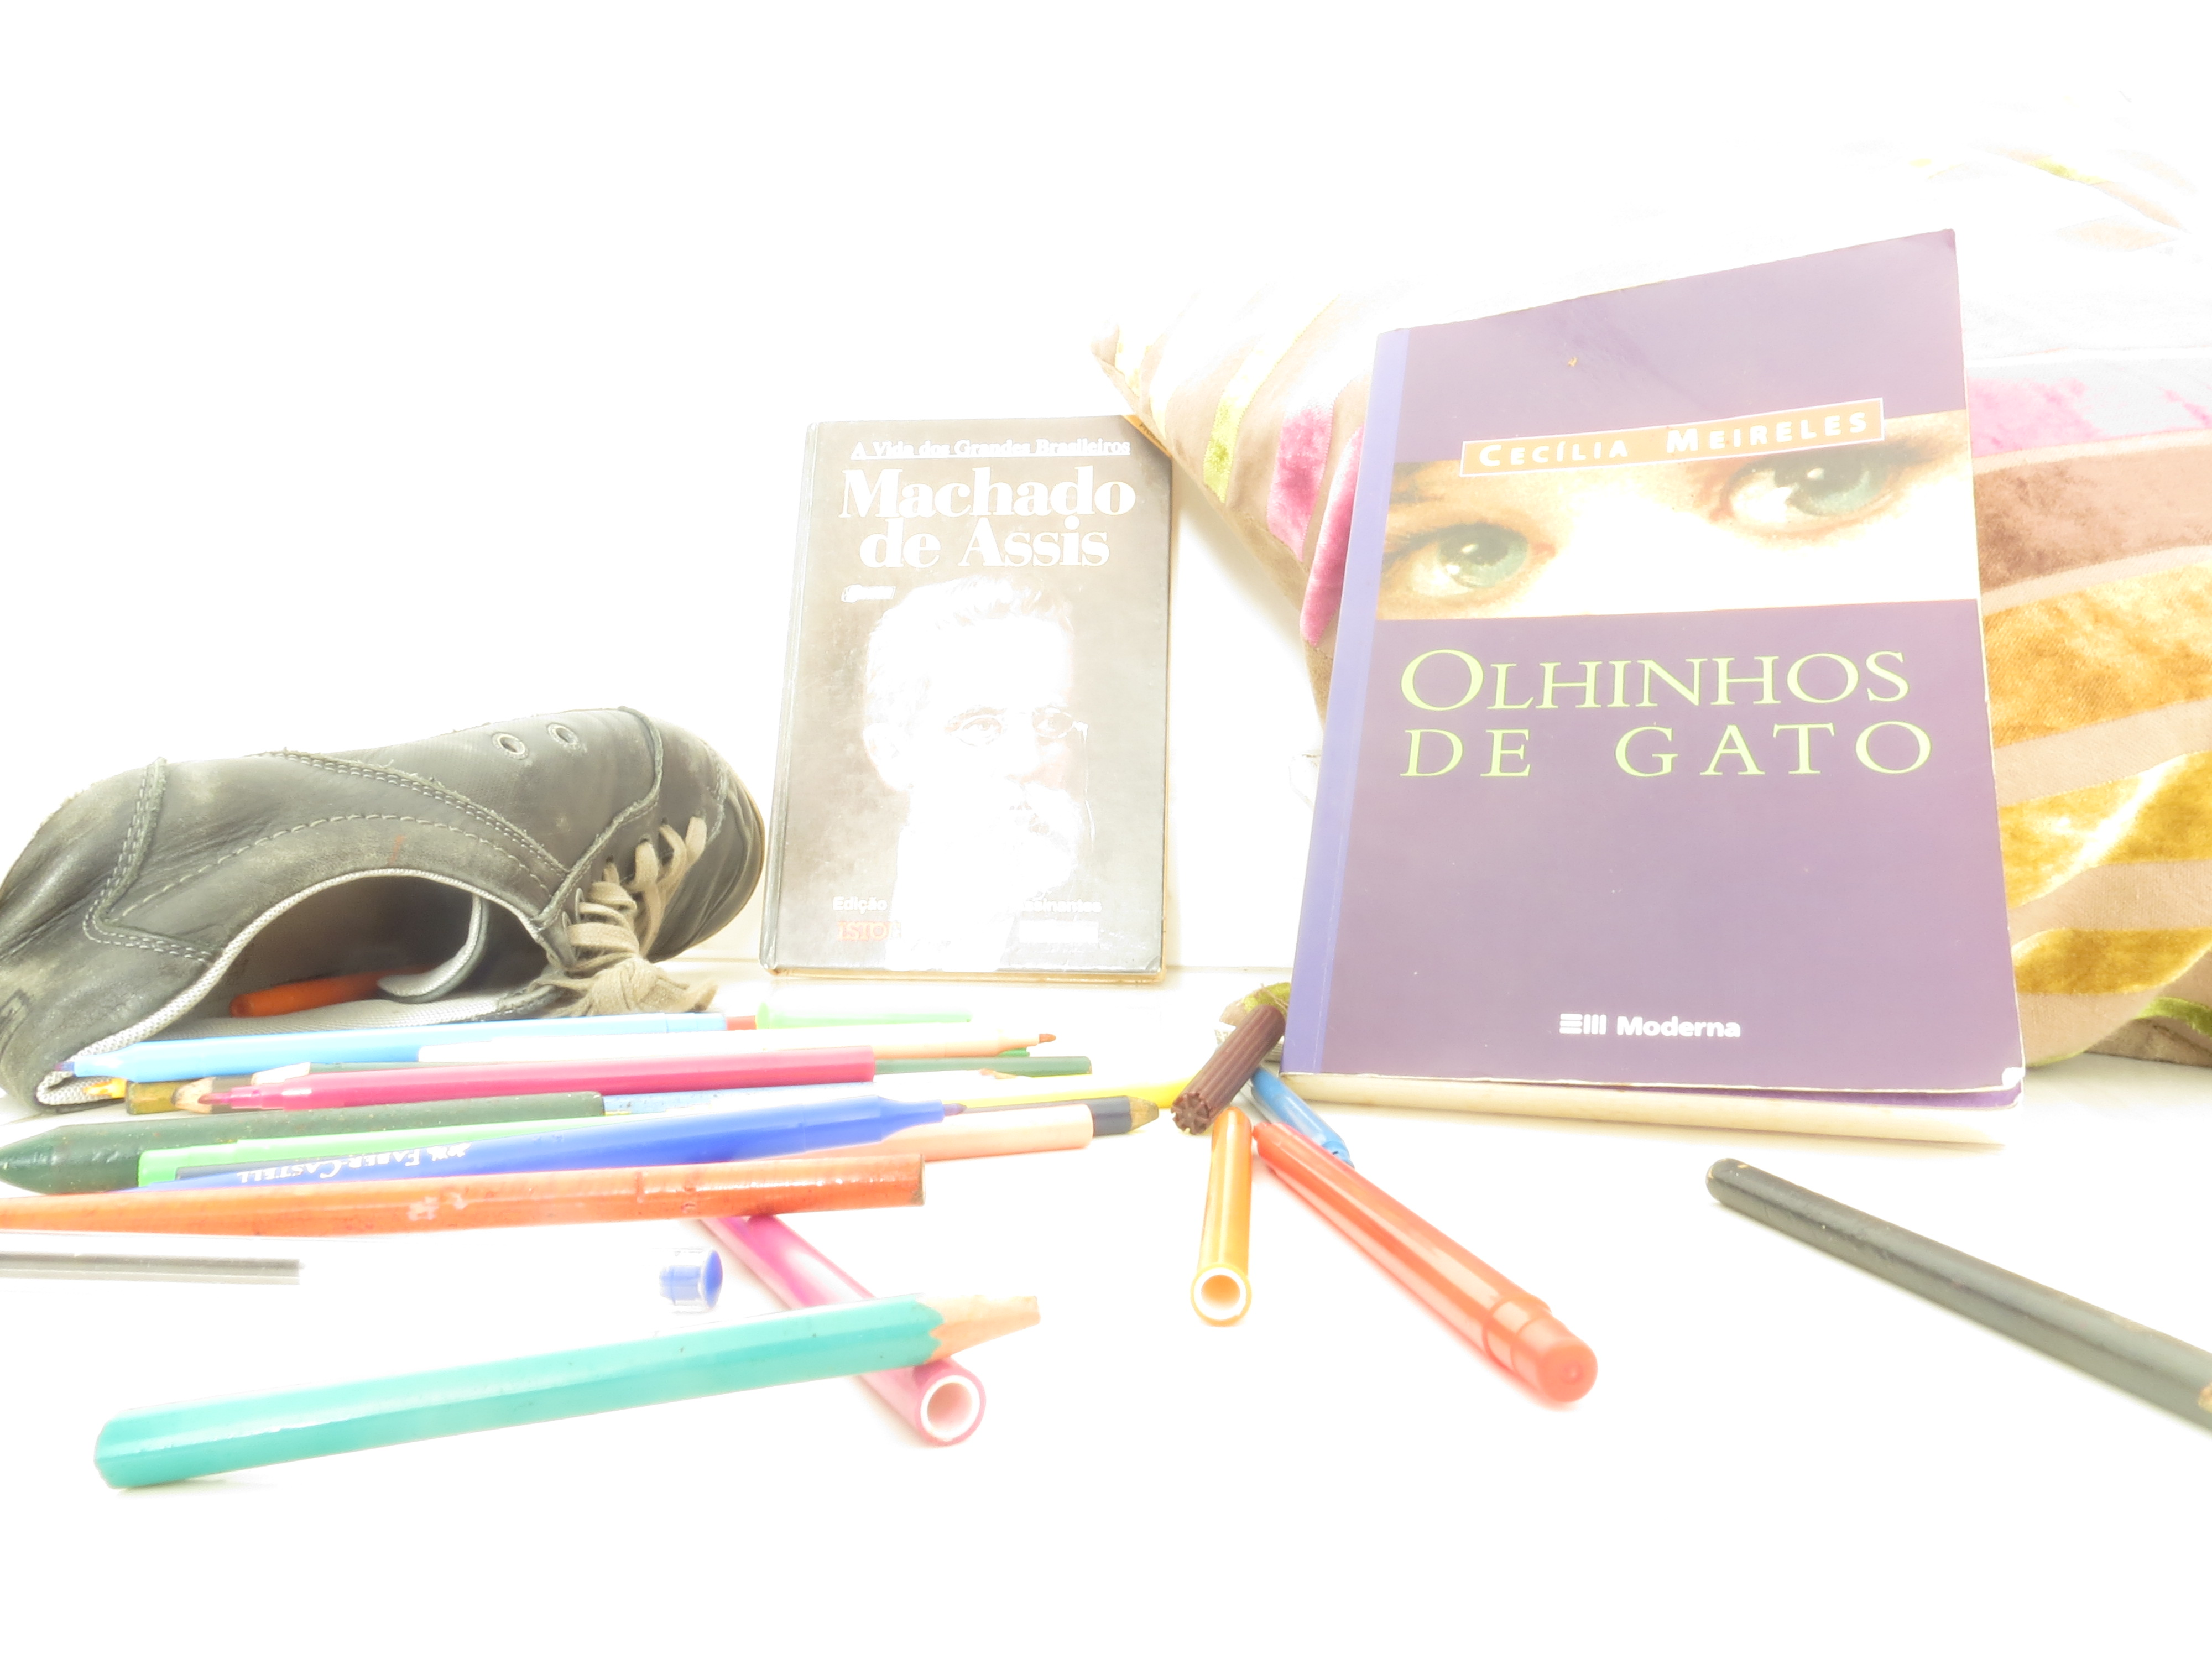
\includegraphics[height=5cm]{CenaOlhinhos/5}
    \label{figBaseOlhihos5}
  }
  \caption{Partes da cena são perdidas em algumas figuras. Porém estas mesmas partes são bem representadas em outras figuras.}
  \label{figBaseOlhinhos}
\end{figure}

\subsubsection{Software para Visualização de Imagens HDR} \label{baseImgPicturenaut}

Para a visualização das imagens HDR geradas, é necessário o uso de software específico. Neste trabalho é utilizado o Picturenaut, disponível no link da Referência \cite{picturenaut}. Este foi escolhido devido a seu fácil manuseio, compatibilidade com diversos tipos de arquivos e por possuir uma ferramenta que realiza tone mapping de imagens HDR.

\subsection{Mann e Picard} \label{metodoMann}
O método proposto por Mann~e~Picard~\cite{mann} parte do pressuposto de que, para ambientes com áreas bem iluminadas e outras pouco iluminadas, as câmeras convecionais acabam perdendo informações por não possuírem faixa dinâmica suficiente para representação de todos os valores de iluminação ali presentes. A solução de alguns fotógrafos para este problema é regular manualmente o tempo de exposição dos sensores da câmera, de forma que a perda seja a menor possível, ou valorizando apenas áreas de seu interesse. A solução proposta pelos autores restringe o problema à captura de várias imagens de uma mesma cena, variando apenas o tempo de exposição, sem que haja movimentação da câmera entre as capturas. Cada imagem possuirá informações relevantes de determinadas áreas da cena, e ao unir essas imagens obtem-se uma imagem com mais informações visíveis do ambiente.
 
 
Para que se possa fazer a união das imagens é necessário saber o valor de iluminação que gerou o mapeamento para um dado pixel da imagem. Para isso, é necessário fazer o cálculo da inversa da função resposta da câmera, que é diferente para cada modelo de câmera no mercado, e muitas vezes é não-linear. Os autores propuseram um algoritmo para inferir a função resposta da câmera e assim calcular a sua inversa.

\subsubsection{Algoritmo para Inferir a Função Resposta} \label{metodoMannAlg}

Para o algoritmo são necessárias duas imagens $a$ e $b$ que foram capturadas em diferentes tempos de exposição, e estáticas uma em relação à outra. Considerando $k$ a razão do tempo de exposição de $b$ em relação ao de $a$ ($k > 1$), o objetivo é encontrar a função resposta $f$ da câmera que capturou as imagens seguindo os seguintes passos:

\begin{itemize}
\item É escolhido um pixel relativamente escuro na imagem $a$ posicionado em $(x_{0}, y_{0})$, denotado por $a(x_{0},y_{0})$. Sabe-se que um valor de irradiação de luz $q_{0}$ gerou o valor desse pixel a partir da aplicação da função resposta $f(q_{0}) = a(x_{0}, y_{0})$. 
\item Localiza-se o pixel na mesma posição na imagem $b$. Como as imagens são estáticas uma em relação a outra, sabe-se que $b(x_{0}, y_{0})$ possui o mesmo valor de irradiação de luz que $a(x_{0}, y_{0})$, porém com um tempo de exposição de $k$ vezes maior. Sendo assim volta-se à imagem $a$ e procura-se um pixel com o mesmo valor de $b(x_{0}, y_{0})$, denominado $a(x_{1}, y_{1}) = f(kq_{0})$.
\item Localiza o pixel $b(x_{1},y_{1})$ na imagem $b$, e procura-se na imagem $a$ um pixel com o valor $b(x_1,y_1)$ denominado $a(x_2, y_2) = f(k² q_0)$.
\item Ao aplicar a lógica do passo anterior sucessivamente para os pontos $(x_2, y_2), (x_3, y_3), ... , (x_n, y_n)$ é feito o mapeamento da não linearidade da função resposta.
\end{itemize}
Uma vez com os pontos encontrados elimina-se o termo $q_{0}$ por meio da mudança de escala, uma vez que não importa a unidade do eixo de irradiação \cite{mann}. Isso leva o nível de irradiação $q_{0}$ a ser considerado uma unidade de irradiação.

O método assume então que a função resposta possui a forma:
\begin{align} \label{eqMannTotal}
	f_{(q)} = \alpha + \beta q ^ \gamma
\end{align}
 Onde $\alpha$ pode ser considerado zero ao subtrair os valores dos pixels pelo valor obtido em uma imagem com tampa da lente colocada. O $\beta$ é um valor de escala e é arbitrário. E o $\gamma$ pode ser inferido atravéz da equação:
	
\begin{align} \label{eqMannGama}
          b(x_{i},y_{i}) &= k^\gamma + a(x_{i},y_{i})
\end{align}


\subsubsection{Geração da Imagem HDR} \label{metodoMannGeracao}

O método proposto pelos autores para geração de uma imagem HDR se baseia na ideia que a derivada da função resposta da câmera em relação ao eixo logarítmico é proporcional à confiabilidade que o pixel apresenta. Sendo assim, para cada pixel da imagem, é feita uma média ponderada da confiabilidade que o pixel apresenta em cada tempo de exposição, possuindo maior peso aquele que possuir maior confiabilidade. Assim, é obtido um pixel HDR que foi formado a partir de informações de todas as exposições.

Seja um conjunto com $N$ imagens alinhadas entre si, variando apenas no tempo de exposição $t_{i}$, $i = 1 ... N$, onde cada imagem possui $M$ pixels representados por $I_{ij}$, $j = 1... M$, cada um com peso $p_{ij}$. A equação para inferir o valor de irradiação do pixel $x_{j}$ é dada por:

\begin{align} \label{eqMannGeracao}
          x_{j} = \frac{\sum\limits_{i \in N}{p_{ij}\frac{f^{-1}(I_{ij})}{t_{i}}}}{\sum\limits_{i \in N}{p_{ij}}}
\end{align}

\subsubsection{Resultados e Discussões} \label{metodoMannResultado}

O método em questão foi implementado na linguagem de programação C++, e foi utilizado um conjunto de imagens capturadas neste trabalho para a verificação dos resultados. Verificou-se que, pelo fato do $\beta$ da equação \ref{eqMannTotal} ser arbitrário, a depender do valor atribuido a ele pode haver uma incompatibilidade entre as funções respostas dos diferentes canais de cores da imagem, como mostrado na Figura \ref{figMannFigErr}.

\begin{figure}[H]
  \centering
  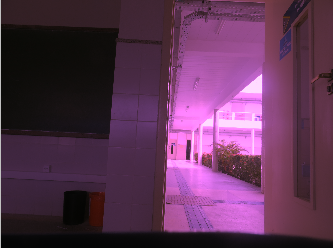
\includegraphics[height=6cm]{Mann/Ruin}
  \caption{Imagem HDR com diferença de escala entre os canais.}
  \label{figMannFigErr}
\end{figure}

Para resolver este problema foi utilizada a mesma solução proposta por Robertson \etal~\cite{robertson}, que estabelece que a função resposta deve sempre mapear o pixel com valor intermediário (128 para pixels com 8 bits) para o valor de uma unidade de luminosidade irradiada. Com essa modificação foi possível obter resultados satisfatórios na união dos canais HDR, conforme mostrado nas Figuras \ref{figMann1}, \ref{figMann2} e \ref{figMann3}.

\begin{figure}[H]
  \centering
  \subfloat[Imagem visualizada com ganho de -9,5EV.]
  {
    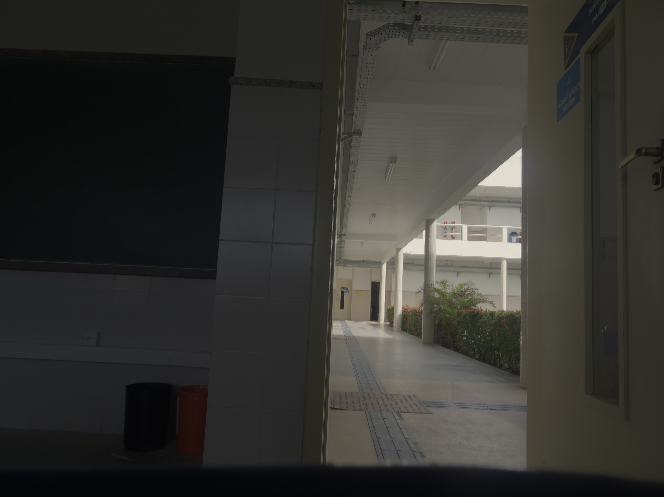
\includegraphics[height=6cm]{Mann/manSala-9,5EV}
    \label{figMann1A}
  }
  \quad %espaco separador
  \subfloat[Imagem visualizada com ganho de -4,8EV.]
  {
    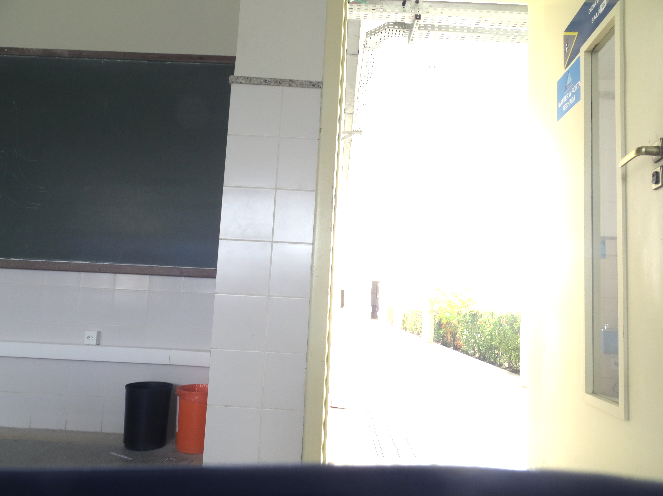
\includegraphics[height=6cm]{Mann/manSala-4,8EV}
    \label{figMann1B}
  }
  \caption{Imagem HDR obtida utilizando o método de Mann e Picard~\protect\cite{mann}.}
  \label{figMann1}
\end{figure}

\begin{figure}[H]
  \centering
  \subfloat[Imagem visualizada com ganho de -3,6EV.]
  {
    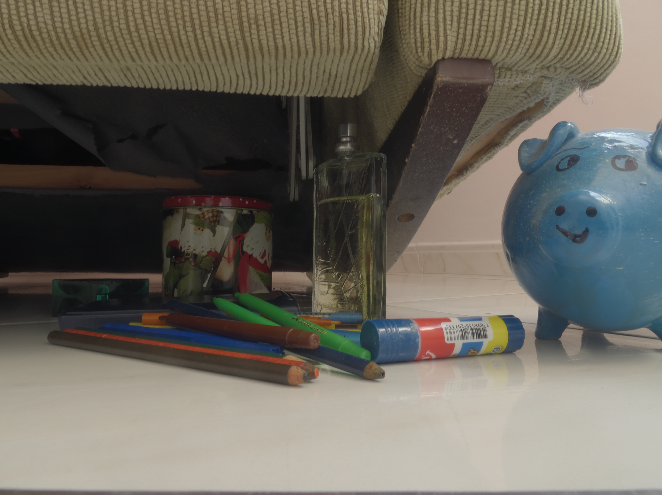
\includegraphics[height=6cm]{Mann/manPorquinho-3,6EV}
    \label{figMann2A}
  }
  \quad %espaco separador
  \subfloat[Imagem visualizada com ganho de -0,4EV.]
  {
    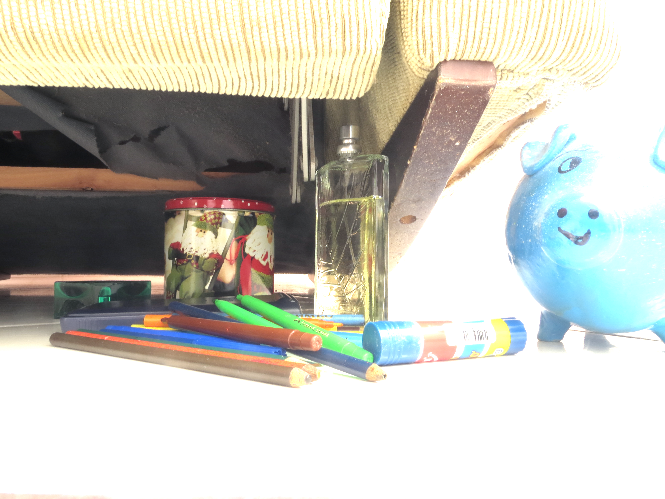
\includegraphics[height=6cm]{Mann/manPorquinho-0,4EV}
    \label{figMann2B}
  }
  \caption{Imagem HDR obtida utilizando o método de Mann e Picard~\protect\cite{mann}.}
  \label{figMann2}
\end{figure}

\begin{figure}[H]
  \centering
  \subfloat[Imagem visualizada com ganho de -2,9EV.]
  {
    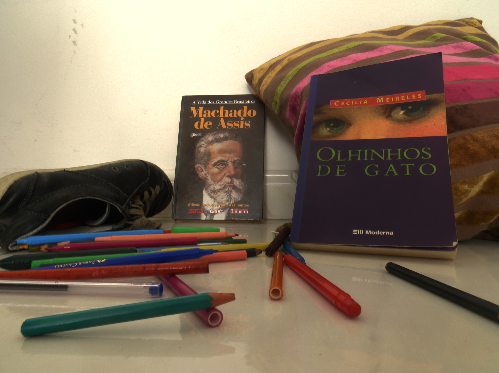
\includegraphics[height=6cm]{Mann/manOlhinhos-2,9EV}
    \label{figMann3A}
  }  
  \quad %espaco separador
  \subfloat[Imagem visualizada com ganho de 0EV.]
  {
    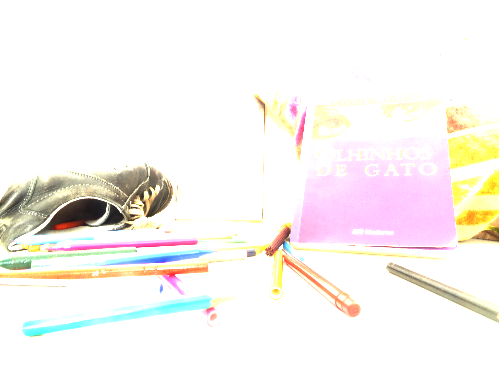
\includegraphics[height=6cm]{Mann/manOlhinhos0EV}
    \label{figMann3B}
  }
  \caption{Imagem HDR obtida utilizando o método de Mann e Picard~\protect\cite{mann}.}
  \label{figMann3}
\end{figure}

A Figura \ref{figMannFR} mostra as funções resposta dos três canais obtidas utilizando o método proposto Mann e Picard \cite{mann}. O eixo das abscissas representa o nível de exposição que elemento sensor da câmera. E o eixo das ordenadas representa o pixel que essa exposição é mapeada ao aplicar a função resposta da câmera, que foi inferida pelo método.

\begin{figure}[H]
  \centering
  \subfloat[Linear.]
  {
    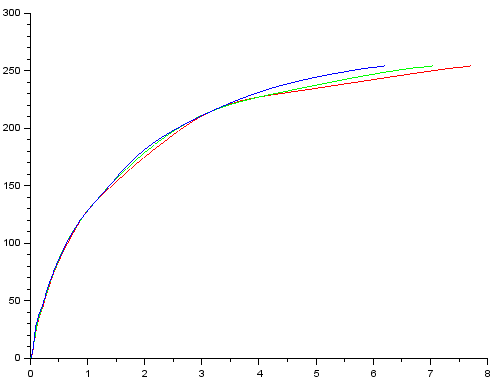
\includegraphics[height=6cm]{Mann/Fr-linear-total}
    \label{figMannFRA}
  }
  \quad %espaco separador
  \subfloat[Logaritmica.]
  {
    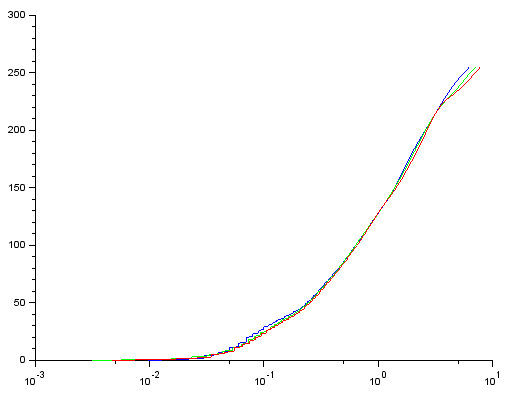
\includegraphics[height=6cm]{Mann/Fr-log-total}
    \label{figMannFRB}
  }
  \caption{Funções resposta da câmera no eixo linear (a) e no eixo logarítmico (b), referentes aos canais vermelho, verde e azul, obtidos com o método de Mann e Picard~\protect\cite{mann}.}
  \label{figMannFR}
\end{figure}
\subsection{Método Robertson} \label{metodoRobertson}

O método proposto por Robertson \etal~\cite{robertson} aborda a geração de imagens HDR de maneira similar ao método proposto por Mann e Picard (Subseção \ref{metodoMann}). Esse método utiliza a derivada da função resposta em um eixo logarítmico como peso e assume que as imagens são estáticas entre si, variando apenas o tempo de exposição. As principais diferenças entre os dois métodos são a postura adotada em relação ao tratamento do ruído e a forma como a função resposta da câmera é inferida. Neste caso a função resposta é inferida por meio de um método iterativo que supõe uma função inicial padrão e então, com uso da relaxação de Gauss-Seidel (vide livro de Ruggiero e Lopes~\cite{livroCalculoNumerico}), aproxima a função resposta de forma a obter um erro abaixo de um limiar estabelecido.

\subsubsection{Geração da Imagem HDR} \label{metodoRobertsonGeracao}

Ao tentar extrair o valor de irradiação de luz ao qual um pixel é mapeado, aplica-se a inversa da função resposta. No entanto, no momento de registro da imagem, vários fatores influenciam para que o valor registrado seja ligeiramente diferente do valor ideal. Isso se dá por conta da presença do ruído no ambiente, que pode ser advindo de fontes diferentes, como corrente de escuro, conversão de analógico para digital entre outros. Assim, a equação da inversa da função resposta da câmera pode ser descrita da seguinte maneira:

\begin{align} \label{eqRobertsonIFR}
	f_{(p_{ij})}^{-1} = I_{p_{ij}} = xt_{i} + N_{ij}
\end{align}
Onde
\begin{itemize}
\item $N_{ij}$ representa os ruídos que tiveram influência na captura do pixel.
\item $x$ é o valor de irradiação de luz real que deseja-se encontrar.
\item $t_{i}$ é o tempo de exposição ao qual o sensor da câmera foi submetido para captura do pixel.
\item $p_{ij}$ é o valor do pixel $j$ da imagem com exposição $t_{i}$.
\end{itemize}

Como o ruído é uma característica específica de cada ambiente/câmera utilizada, modelar o problema de forma a caracterizar cada ruído é uma tarefa bastante complexa. Sendo assim, este método trata o ruído sob o ponto de vista de uma distribuição Gaussiana com média zero para simplificar a modelagem.

Utilizando-se de operações algébricas para calcular o erro de um valor de iluminação inferido em relação ao valor real, obtém-se a seguinte equação:

\begin{align} \label{eqRobertsonErr}
	O(x) = \sum\limits_{i,j}{w_{ij}(I_{p_{ij}} - x_{ij}t_{i})^2}
\end{align}

Essa equação representa o erro quadrático entre o valor inferido e o valor obtido pela inversa. Fazendo o gradiente de $O(x)$ tender a zero, Robertson chegou à seguinte equação para inferência do valor de irradiação de luz:

\begin{align} \label{eqRobertsonGeracao}
	x^{*}_j = \frac{\sum\limits_{i \in N}{w_{ij}t_{i}I_{p_{ij}}}}{\sum\limits_{i \in N}{w_{ij}t_{ij}^{2}}}
\end{align}
Onde
\begin{itemize}
\item $x^{*}_j$ é o valor de irradiação de luz inferido.
\item O peso $w_{ij}$ é obtido pela derivada da função resposta em relação um eixo logarítmico. 
\end{itemize}

O conjunto de valores $x^{*}_j$, que são gerados a partir da convolução das imagens de entrada, formam a imagem HDR final.

\subsubsection{Algoritmo para Inferir a Função Resposta} \label{metodoRobertsonAlg}

Na maioria dos casos, não se sabe a função resposta de uma câmera e por isso ela deve ser estimada \cite{robertson}. Para a estimativa da função resposta é necessária a minimização da função do erro quadrático, dada pela seguinte equação:

\begin{align} \label{eqRobertsonErr2}
	O(I,x) = \sum\limits_{i,j}{w_{ij}(I_{p_{ij}} - x_{ij}t_{i})^2}
\end{align}

Essa equação é parecida com a Equação \ref{eqRobertsonErr}, porém com uma variável $I$ de entrada que também será inferida. Como não se sabe o valor de irradiação $x_{ij}$ nem a função resposta para calcular o valor de $I_{p_{ij}}$, utiliza-se o método de relaxação de Gauss-Seidel para inferir ambas as variáveis simultaneamente. Também é necessário estabelecer uma função para mapear os pesos uma vez que, como não se sabe a função resposta da câmera, não há como obter a sua derivada. Robertson propôs a seguinte função para definir os pesos \cite{robertson2}:

\begin{align} \label{eqRobertsonErr3}
	w_{ij} = e^{-4\frac{(p_{ij}-127.5)^2}{127.5^2}}
\end{align}

O método de inferência da fução resposta possui um passo inicial e um conjunto de passos iterativos, descritos a seguir.

\begin{itemize}
\item Passo inicial:

Estabelece-se a função resposta inicial como sendo uma função linear com o valor $I_{128}^{*(0)} = 1.0$, e o valor de $x^{*(0)}$ é obtido aplicando a equação \ref{eqRobertsonGeracao}.

\item Passos iterativos:

Para cada iteração $l$ são feitos os seguintes passos:
\subitem \textbf{1.} Considerando $E_m$ o conjunto de pixels que possuem o valor igual a $m$, faz-se o relaxamento de $I^{*(l)}$ aplicando a seguinte Equação para inferi-lo:
\begin{align} \label{eqRobertsonIteracaoFR}
	I^{*(l)}_m = \frac{\sum\limits_{(i,j) \in E_m}{w_{ij}t_{i}x_{j}^{*(l-1)}}}{\sum\limits_{(i,j) \in E_m}{w_{ij}}}
\end{align}
\subitem \textbf{2.} Normaliza-se $I_{p_{ij}}$ de forma que $I_{128}$ seja uma unidade.
\subitem \textbf{3.} É feita a relaxação de $x^{*(l)}$ com base na seguinte equação:
\begin{align} \label{eqRobertsonIteracaoHDR}
	x^{*(l)}_j = \frac{\sum{_i w_{ij}t_{i}I^{*(l)}_{p_{ij}}}}{\sum{_i w_{ij}t_{i}^2}}
\end{align}
\end{itemize}

Dessa forma, a função resposta e a imagem HDR vão sendo inferidas simultaneamente, e quando as modificações feitas no passo iterativo da Equação \ref{eqRobertsonIteracaoFR} forem menores que um limiar predefinido, o passo iterativo é terminado.

Ao final do método, possui-se um conjunto de valores $\{I_{p_{ij}}\}$ que representam informações da função resposta da câmera. Como este conjunto é discreto, há a necessidade de efetuar uma interpolação utilizando a técnica da Spline cúbica (vide livro de Ruggiero e Lopes~\cite{livroCalculoNumerico}) para obtenção da função resposta final como ilustrado na Figura \ref{figRobertsonPontos}. 

\begin{figure}[H]
  \centering
  \subfloat[Ilustração dos pontos utilizados na interpolação.]
  {
    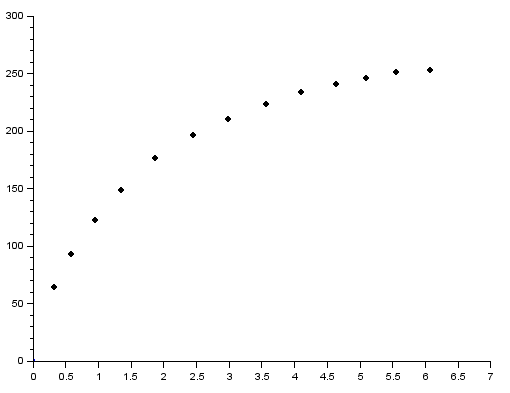
\includegraphics[height=6cm]{Robertson/Pontos}
    \label{figRobertsonPontosA}
  }
  \quad %espaco separador
  \subfloat[Função resposta obtida com a interpolação.]
  {
    \includegraphics[height=6cm]{Robertson/fr-linear-azul}
    \label{figRobertsonPontosB}
  }
  \caption{Interpolação da função resposta do canal azul da câmera, utilizando o método da Spline cúbica.}
  \label{figRobertsonPontos}
\end{figure}

\subsubsection{Resultados e Discussões} \label{metodoRobertsonResultado}

O método em questão foi implementado na linguagem de programação C++, assim como o método de interpolação por spline cúbica. Os resultados são mostrados nas Figuras \ref{figRobertsonDidatica}, \ref{figRobertsonPorquinho} e \ref{figRobertsonOlhinhos}.

\begin{figure}[H]
  \centering
  \subfloat[Imagem visualizada com ganho de -11,0EV.]
  {
    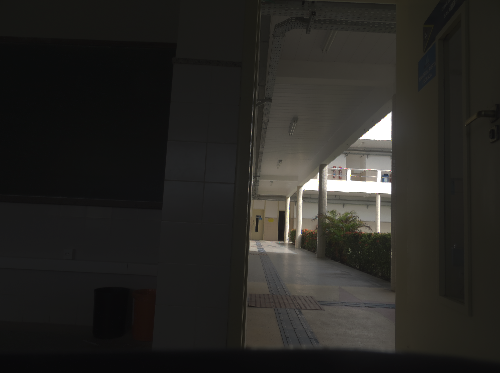
\includegraphics[height=6cm]{Robertson/robertsonSala-11,0EV}
    \label{figRobertsonDidaticaA}
  }
  \quad %espaco separador
  \subfloat[Imagem visualizada com de ganho -4,3EV.]
  {
    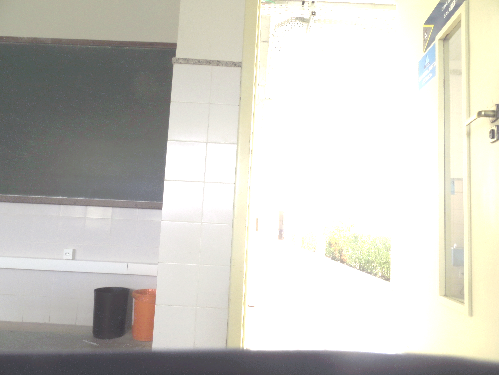
\includegraphics[height=6cm]{Robertson/robertsonSala-4,3EV}
    \label{figRobertsonDidaticaB}
  }
  \caption{Imagem HDR gerada utilizando o método de Robertson~\etal~\protect\cite{robertson}.}
  \label{figRobertsonDidatica}
\end{figure}

\begin{figure}[H]
  \centering
  \subfloat[Imagem visualizada com ganho de -4,3EV.]
  {
    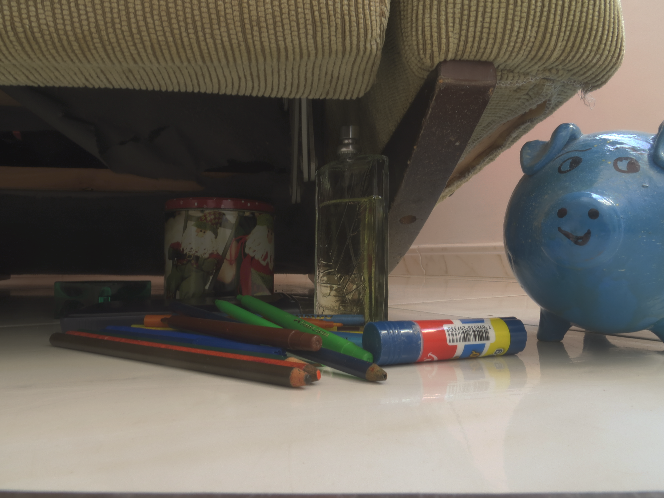
\includegraphics[height=6cm]{Robertson/robertsonOtima-4,3EV}
    \label{figRobertsonPorquinhoA}
  }
  \quad %espaco separador
  \subfloat[Imagem visualizada com ganho de -2,0EV.]
  {
    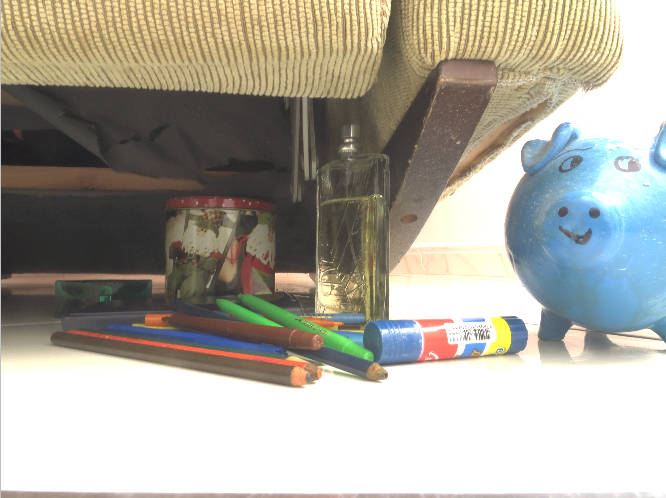
\includegraphics[height=6cm]{Robertson/robertsonOtima-2,0EV}
    \label{figRobertsonPorquinhoB}
  }
  \quad %espaco separador
  \subfloat[Imagem visualizada com ganho de 0EV.]
  {
    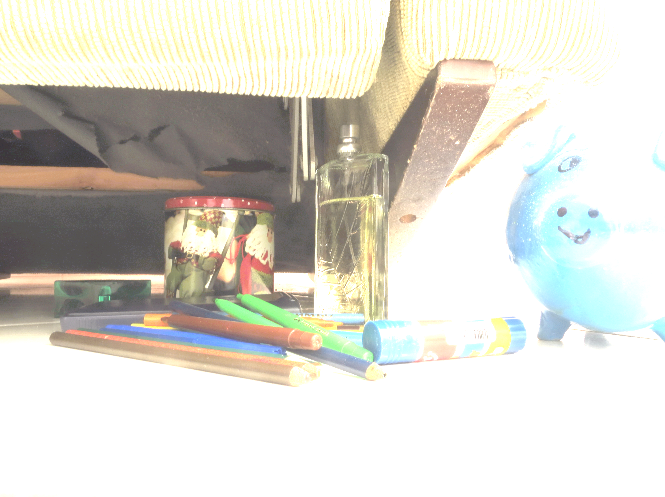
\includegraphics[height=6cm]{Robertson/robertsonOtima0,0EV}
    \label{figRobertsonPorquinhoC}
  }
  \caption{Imagem HDR gerada utilizando o método de Robertson~\etal~\protect\cite{robertson}.}
  \label{figRobertsonPorquinho}
\end{figure}


\begin{figure}[H]
  \centering
  \subfloat[Imagem visualizada com ganho de -4,3EV.]
  {
    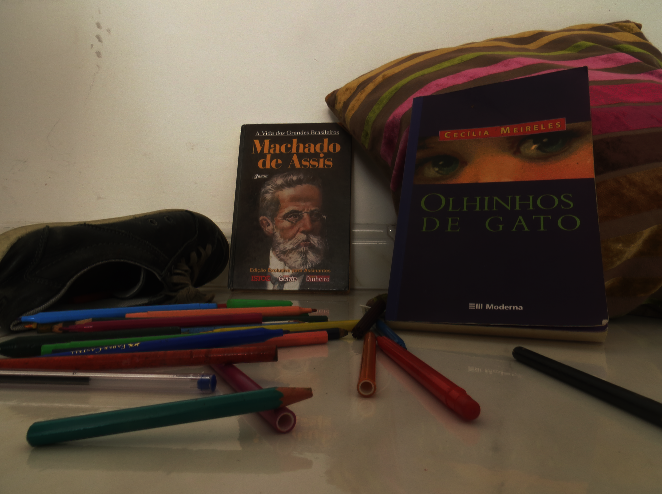
\includegraphics[height=6cm]{Robertson/robertsonOlhinhos-4,3EV}
    \label{figRobertsonOlhinhosA}
  }
  \quad %espaco separador
  \subfloat[Imagem visualizada com ganho de -2,7EV.]
  {
    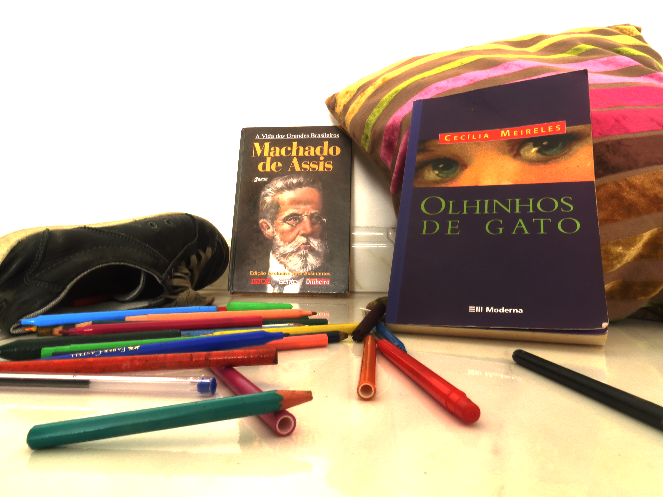
\includegraphics[height=6cm]{Robertson/robertsonOlhinhos-2,7EV}
    \label{figRobertsonOlhinhosB}
  }
  \quad %espaco separador
  \subfloat[Imagem visualizada com ganho de -0,4EV.]
  {
    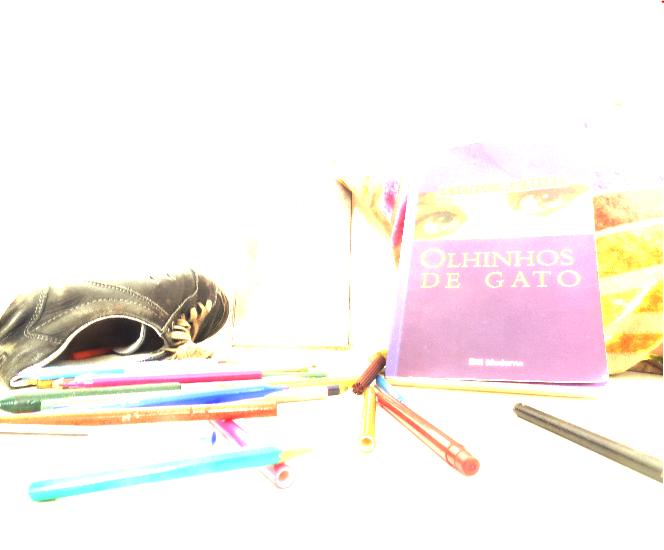
\includegraphics[height=6cm]{Robertson/robertsonOlhinhos-0,4EV}
    \label{figRobertsonOlhinhosC}
  }
  \caption{Imagem HDR gerada utilizando o método de Robertson~\etal~\protect\cite{robertson}.}
  \label{figRobertsonOlhinhos}
\end{figure}


\begin{figure}[H]
  \centering
  \subfloat[Imagem HDR gerada]
  {
    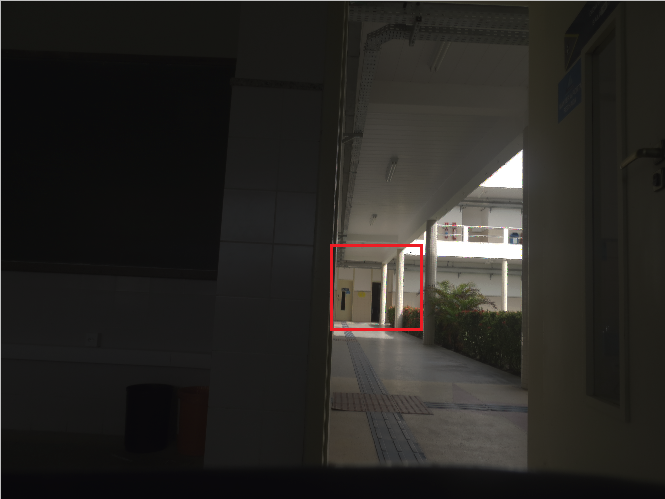
\includegraphics[height=6cm]{Robertson/Sala}
    \label{figRobertsonSalaA}
  }
  \quad %espaco separador
  \subfloat[A ampliação mostrou a presença de ruído na imagem]
  {
    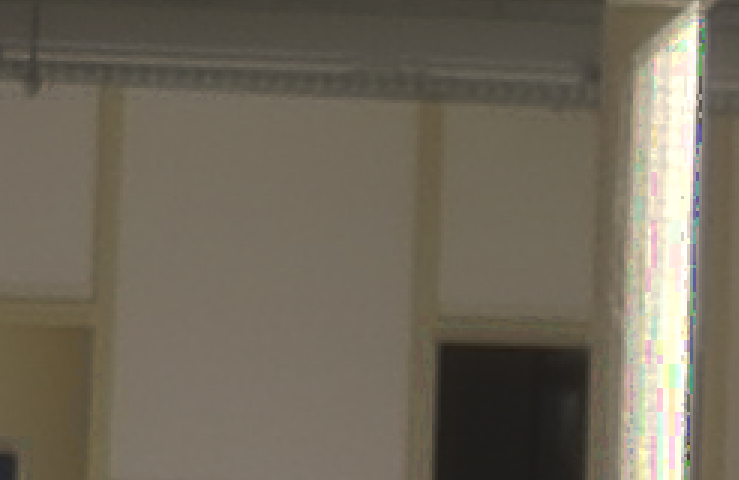
\includegraphics[height=6cm]{Robertson/Ruido}
    \label{figRobertsonSalaB}
  }
  \caption{Imagem HDR gerada utilizando o método de Robertson~\etal~\protect\cite{robertson}, que apresentou ruído em partes com muita irradiação de luz.}
  \label{figRobertsonSala}
\end{figure}

Notou-se que áreas com exposição muito elevada apresentaram ruído mais perceptível, como mostrado na Figura \ref{figRobertsonSalaB}. E a Figura \ref{figRobertsonFR} mostra as funções resposta dos diferentes canais, obtidas utilizando o método proposto.

\begin{figure}[H]
  \centering
  \subfloat[Eixo linear]
  {
    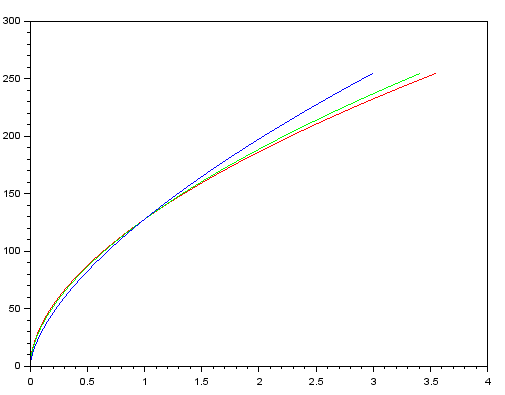
\includegraphics[height=6cm]{Robertson/fr-linear-total}
    \label{figRobertsonFRA}
  }
  \quad %espaco separador
  \subfloat[Eixo logarítmico]
  {
    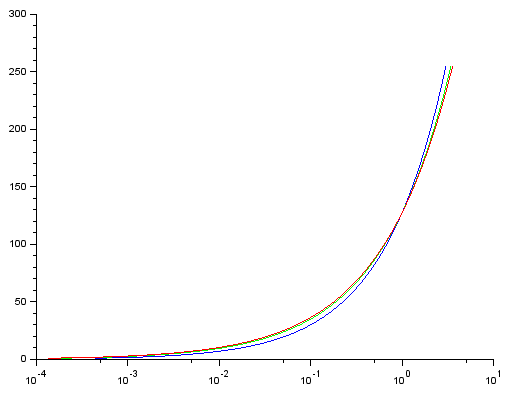
\includegraphics[height=6cm]{Robertson/fr-log-total}
    \label{figRobertsonFRB}
  }
  \caption{Funções resposta da câmera relativas aos diferentes canais de cores.}
  \label{figRobertsonFR}
\end{figure}


\subsection{Método Sen} \label{metodoSen}

O método proposto por Sen~\etal~\cite{hdrMovimento}, aborda a geração de imagens HDR sob uma ótica bastante diferenciada dos outros métodos citados anteriormente, apesar de partir do mesmo pressuposto da união de várias imagens LDR em diferentes tempos de exposição para gerar uma imagem HDR. Um dos princípios básicos deste método é a robustez quanto ao movimento dos elementos das imagens, característica essa que nos outros métodos era assumida como sendo estática.

No processo de captura de uma sequência de várias imagens, assumir que uma imagem e os elementos contidos na mesma estarão estáticos em relação às outras imagens só é possível para ambientes bastante controlados. Para isso há a necessidade de que os objetos da cena não sejam móveis, e é requerido o uso de equipamentos mais sofisticados como tripé da câmera para mantê-la fixa e/ou uso de câmeras controladas remotamente. Estes casos são bastante específicos e não correspondem à realidade de grande parte dos usuários de câmeras digitais convencionais. Muitos destes possuem como única alternativa, a captura das imagens sem tripé, sem software, onde as cenas capturadas possuem uma dinâmica bem diferente de um ambiente estático.

O método em questão se utiliza do princípio de minimização de energia para inferir, a partir de uma imagem de referência e de várias imagens LDR, como seria o registro da imagem de referência se esta fosse capturada com os tempos de exposição das outras imagens. Simultaneamente o algoritmo gera a imagem HDR e cópias da imagem de referência em diferentes tempos de exposição. Utilizando a imagem HDR obtida o algoritmo verifica e corrige a qualidade das imagens LDR que a gerou. Estas imagens com qualidade melhorada geram uma imagem HDR de melhor qualidade. Este ciclo iterativo continua até atingir um limiar.

Ao final, além da imagem HDR, o método gera um conjunto de imagens LDR que conservam os detalhes da imagem de referência mas com diferentes níveis de exposição, ou seja, gera imagens estáticas entre si em diferentes tempos de exposição, o que possibilita o uso destas como entrada para os métodos citados nas Seções \ref{metodoMann} e \ref{metodoRobertson}.

\subsubsection{Modelagem do Problema} \label{MetodoSenModelo}

Seja um conjunto de $N$ imagens LDR $(L_1,L_2,..,L_N)$, onde uma destas é a imagem de referência $L_{ref}$ . Para que o problema possa ser trabalhado como minimização de energia as seguintes propriedades da imagem HDR $H$, que será inferida, devem ser satisfeitas:

\begin{itemize}
	\item Ao mapear um valor de irradiação de $H$ para o tempo de exposição da imagem de referência, o valor mapeado deve ser próximo ao valor do pixel da imagem de referência.
	\item Ao mapear um pixel, propriamente exposto (mensurado por uma função expecífica $\alpha$) da imagem de referência para o domínio de irradiação linear, este deve possuir um valor próximo ao valor de irradiação de $H$.
	\item A imagem de referência deve ser utilizada na composição da imagem HDR quando essa estiver propriamente exposta, caso contrário as outras imagens HDR devem assumir participação na inferência do valor de irradiação com base na múltipla similaridade bidirecional (MBDS), i.e., versão do conceito similaridade bidirecional para tratar múltiplas entradas.
\end{itemize}

Sendo assim a equação da energia é dada pela junção destes fatores como segue:
 
\begin{align} \label{eqSenEnergia}
	E(H) = \sum\limits_{p \in pixels}{[\alpha_{ref_{(p)}}.(h(L_{ref})_{(p)} - H_{(p)})^2 + (1-\alpha_{ref_(p)}).E_{MBDS}(H|L_1,..,L_N)]}
\end{align}
Onde
\begin{itemize}
	\item $E(H)$ é a energia, que deve ser diminuida ao máximo para maior confiabilidade da imagem HDR $H$.
	\item $\alpha_{ref_{(p)}}$ é uma função de peso que indica quão bem exposto um pixel da imagem de referência está.
	\item $h(L)$ mapeia uma imagem $L$ para o domínio de irradiação linear. 
\end{itemize}

Considerando que a equação de energia receberá como entrada um conjunto de imagens LDR $\{I_k\}, k~=~1..N$, onde cada $I_k$ é o mapeamento da imagem HDR $H$ para o tempo de exposição $k$, os autores do método chegaram à seguinte equação de energia:

\begin{equation} \label{eqSenEnergia2}
\begin{split}
	E(H,I_1,..,I_N) = &\underset{p \in pixels}{\sum{}}[\alpha_{ref_{(p)}}.(h(L_{ref})_{(p)} - H_{(p)})^2 +\\
		   &(1-\alpha_{ref_(p)}).\underset{k=1}{\overset{N}{\sum{}}}MBDS(I_k|g^k(L_1),..,g^k(L_N)) +\\
		   &(1-\alpha_{ref_(p)}).\underset{k=1}{\overset{N}{\sum{}}}\Lambda(I_k)_{(p)}.(h(I_k)_{(p)} - H_{(p)})^2]
\end{split}
\end{equation}

Onde

\begin{itemize}
	\item $\Lambda$ é uma função de peso que indica a relevância do pixel para a imagem HDR.
	\item $g^k(L_i)$ mapeia a imagem LDR $L$ com exposição $i$ para uma imagem LDR equivalente com exposição $k$.
\end{itemize}

Sendo assim, a equação pode ser solucionada através de um método iterativo que infere simultaneamente os $H$ e os $\{I_k\}$ seguindo os seguintes passos:

\begin{itemize}
	\item Minimiza-se a equação para $I_1,..,I_N$, usando primeiramente a procura dos melhores fragmentos para resolver o MBDS. E então para cada $I_k$ combina com o mapeamento de $H$ anterior para a exposição $k$, para que eles possuam gradualmente mais informações da imagem de referência.
	\item Minimiza-se então a equação quanto ao valor $H$. Primeiramente mapeia-se a irradiação linear de todos os $\{I_k\}$ e faz-se a combinação dos mesmos para obter $\overset{*}{H}$, como mostra a equação~\ref{eqSenGeracao}. Após isso o valor de $\overset{*}{H}$ é combinado com a imagem de referência mapeada para o domínio de irradiação linear para obter o novo valor da imagem HDR $H$ como mostrado na equação~\ref{eqSenTotal}.
\end{itemize}

\begin{equation} \label{eqSenGeracao}
	\overset{*}{H}_{(p)} = \frac{\sum\limits_{k = 1}^N{\Lambda(I_{k_{(p)}})h(I_k)_{(p)}}}{\sum\limits_{k = 1}^N{\Lambda(I_{k_{(p)}})}}
\end{equation}

\begin{equation} \label{eqSenTotal}
	H_{(p)} = \alpha_{ref_{(p)}}.h(L_{ref})_{(p)} + (1-\alpha_{ref_{(p)}}).\overset{*}{H}_{(p)}
\end{equation}

Esses passos são repetidos até atingir um critério de convergência.

\subsubsection{Especificidades de Implementação} \label{MetodoSenImplementacao}

Para implementação do método foi utilizada a própria implementação disponibilizada pelos autores \cite{hdrMovimento}. Para o correto funcionamento deste há a necessidade de efetuar um preprocessamento nas imagens para colocá-las no domínio linear. Para isso é necessário o conhecimento da função resposta da câmera, pois a partir de sua inversa calcula-se o mapeamento de um pixel (geralmente domínio não-linear) para o domínio linear. Uma vez com a imagem linearizada aplica-se uma correção gama de 2.2 para aumentar a eficácia do algoritmo.

Para a primeira iteração do algoritmo, é necessária a definição do conjunto de imagens de entrada ${I_k}$ como sendo $I_k \leftarrow g^k(L_{ref})$. Para poder definir melhor quais imagens influenciam mais a geração da imagem HDR, os autores utilizaram um conceito de pesos extras na Equação \ref{eqSenTotal}, de forma que imagens com alta exposição não contribuam com pixels muito saturados e imagens com baixa exposição não contribuam com pixels de baixa intensidade.

Outra otimização feita é a implementação de fases do algoritmo relativas a escalas de forma que a correspondência é feita gradualmente de uma baixa resolução para uma alta resolução.

\subsubsection{Resultados e Discussões} \label{MetodoSenResultado}

Notou-se que ao utilizar imagens com alta resolução o processamento era longo e com consumo de memória excessivo. Para o caso em que foi testado, num computador com memória RAM de 4GB, utilizando imagens de 4000x3000 pixels, não foi possível a execução do método pois a mémoria era isuficiente para o processo, sendo assim necessário o redimensionamento das imagens para 2000x1500 pixels.

O método foi testado utilizando o conjunto de imagens mostrado na seção \ref{metodoBaseImg}. Os resultados são mostrados nas Figuras \ref{figSenSala}, \ref{figSenPorquinho} e \ref{figSenOlhinhos}. Apesar da ausência de fantasmas nas imagens, algumas delas, conforme mostrado na Figura \ref{figSenSalaB}, possuíram artefatos que se assemelham a uma quantização das cores quando o ganho é relativamente alto.

\begin{figure}[H]
  \centering
  \subfloat[Imagem visualizada com ganho de $-9,8$EV.]
  {
    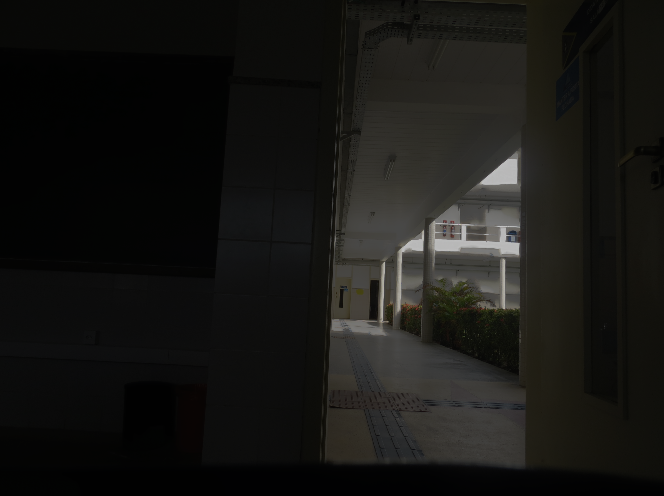
\includegraphics[height=6cm]{Sen/senSala-9,8EV}
    \label{figSenSalaA}
  }
  \quad %espaco separador
  \subfloat[Imagem visualizada com ganho de $-1,1$EV.]
  {
    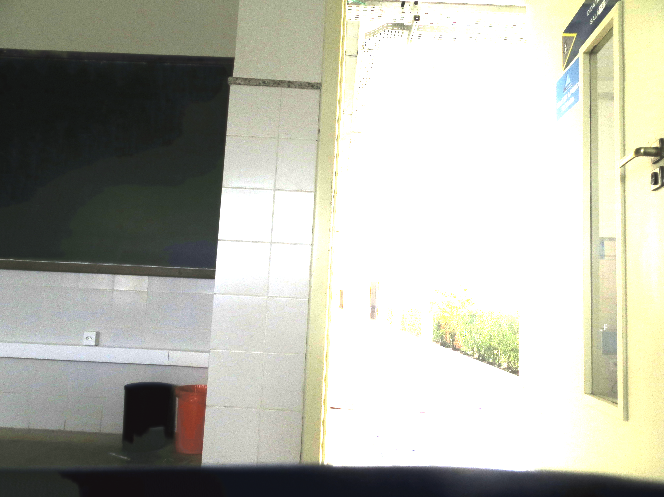
\includegraphics[height=6cm]{Sen/senSala-1,1EV}
    \label{figSenSalaB}
  }
  \caption{Imagem HDR gerada utilizando o método de Sen~\etal~\protect\cite{hdrMovimento}.}
  \label{figSenSala}
\end{figure}

\begin{figure}[H]
  \centering
  \subfloat[Imagem visualizada com ganho de $-1,3$EV.]
  {
    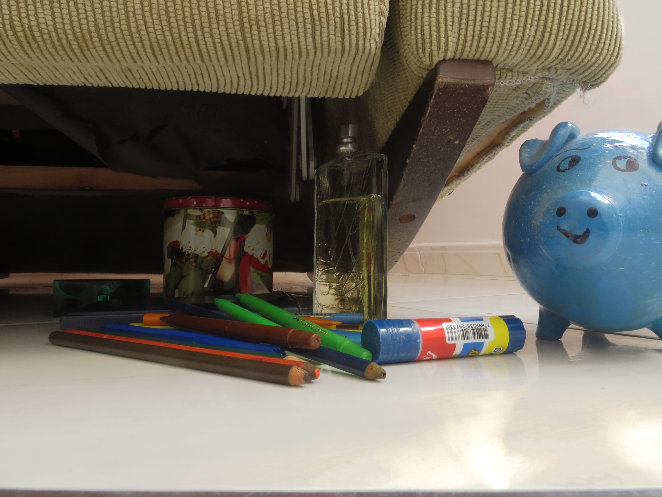
\includegraphics[height=6cm]{Sen/senPorquinho-1,3EV}
    \label{figSenPorquinhoA}
  }
  \quad %espaco separador
  \subfloat[Imagem visualizada com ganho de $2,5$EV.]
  {
    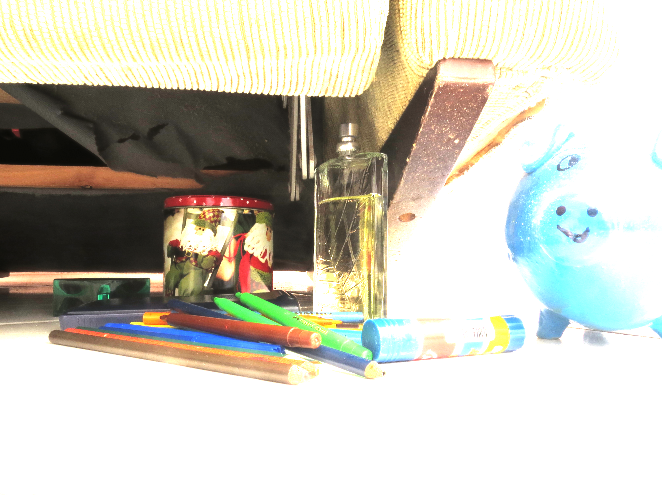
\includegraphics[height=6cm]{Sen/senPorquinho2,5EV}
    \label{figSenPorquinhoB}
  }
  \caption{Imagem HDR gerada utilizando o método de Sen~\etal~\protect\cite{hdrMovimento}.}
  \label{figSenPorquinho}
\end{figure}

\begin{figure}[H]
  \centering
  \subfloat[Imagem visualizada com ganho de $-0,6$EV.]
  {
    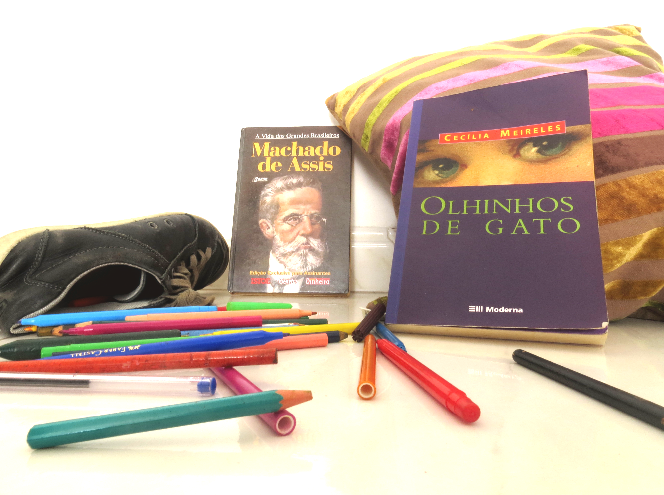
\includegraphics[height=6cm]{Sen/senOlhinhos-0,6EV}
    \label{figSenOlhinhosA}
  }
  \quad %espaco separador
  \subfloat[Imagem visualizada com ganho de $-3,4$EV.]
  {
    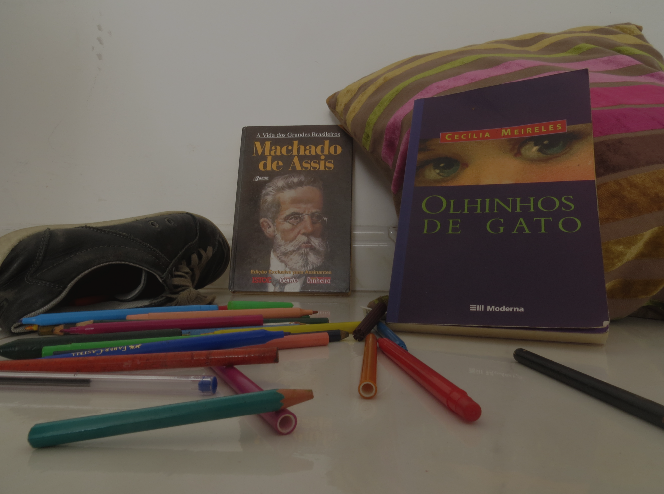
\includegraphics[height=6cm]{Sen/senOlhinhos-3,4EV}
    \label{figSenOlhinhosB}
  }
  \quad %espaco separador
  \subfloat[Imagem visualizada com ganho de $3,6$EV.]
  {
    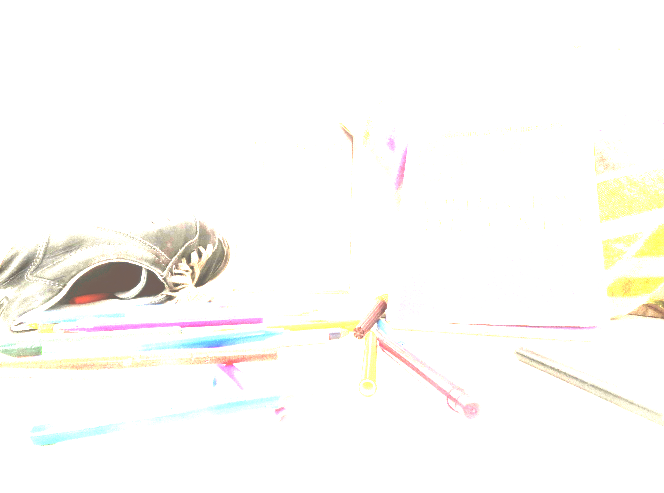
\includegraphics[height=6cm]{Sen/senOlhinhos3,6EV}
    \label{figSenOlhinhosC}
  }
  \caption{Imagem HDR gerada utilizando o método de Sen~\etal~\protect\cite{hdrMovimento}.}
  \label{figSenOlhinhos}
\end{figure}
\section{Discussões} \label{discussoes}

Com os resultados alcançados, notou-se que todos os métodos atingiram os resultados esperados (geração de imagens HDR), cada qual com suas vantagens e desvantagens. Nesta seção serão abordadas as questões referentes a cada método de geração de imagens HDR abordado neste documento.

\subsection{Método Mann} \label{discussaoMann}
\subsubsection{Vantagens}
\begin{itemize}
	\item Possui a inferência da função resposta mais rápida.
	\item Em alguns casos mostrou resultado mais consistente que o método de Robertson \etal \cite{robertson}.
\end{itemize}
\subsubsection{Desvantagens}
\begin{itemize}
	\item As imagens de entrada não devem apresentar movimento entre suas capturas.
	\item A inferência da função resposta leva em conta apenas alguns pixels e não todos.
	\item A inferência da função resposta leva em conta apenas 2 imagens.
	\item A falta de especificação da escala na inferência da função resposta leva, em alguns casos, à incoerência na união dos canais de cores.
\end{itemize}


\subsection{Método Robertson} \label{discussaoRobertson}
\subsubsection{Vantagens}
\begin{itemize}
	\item A inferência da função resposta leva em conta todas as imagens.
	\item A inferência da função resposta leva em conta todos os pixels da imagem.
\end{itemize}
\subsubsection{Desvantagens}
\begin{itemize}
	\item Na implementação feita algumas imagens HDR apresentaram ruído.
	\item As imagens de entrada não devem apresentar movimento entre suas capturas.
\end{itemize}

\subsection{Método Sen} \label{discussaoSen}
\subsubsection{Vantagens}
\begin{itemize}
	\item Robustez quanto ao movimento nas imagens.
\end{itemize}
\subsubsection{Desvantagens}
\begin{itemize}
	\item Necessita de função resposta.
	\item Método mais lento de obtenção de imagens HDR.
	\item Não suporta imagens em alta resolução.
\end{itemize}

Tanto o método proposto por Mann e Picard~\cite{mann}, quanto o proposto Robertson~\etal~\cite{robertson}, supõem que a câmera estará totalmente estática entre a captura das imagens. Para que isso seja verdade, há a necessidade de equipamentos mais sofisticados como tripé e software de captura por computador e de um ambiente muito controlado. 

Tendo em vista que usuários comuns de câmeras digitais não costumam possuir equipamento que possibilite a inexistência de movimento entre a captura de imagens. O método mais aplicável para este cenário se mostra o proposto por Sen~\etal~\cite{hdrMovimento}, por se tratar de um método mais robusto quanto ao movimento. Sendo assim, este será o método utilizado na próxima etapa deste trabalho para a obtenção de nuvem de pontos a partir de imagens HDR.


\chapter{Obtenção de Nuvem de Pontos a partir de Imagens HDR} \label{parteNuvem}

Neste capítulo serão abordados conceitos relacionados à geração de nuvem de pontos a partir de imagens HDR. Para isso serão introduzidos trabalhos e técnicas relacionados ao assunto, assim como softwares e ferramentas utilizadas para geração de nuvens de pontos convencionais. Será então proposto um método para aquisição efetiva da nuvem de pontos a partir de imagens HDR.


\section{Revisão Bibliográfica} \label{revisaoPontos}

Dentre os principais assuntos que se relacionam ao tema deste capítulo, pode-se destacar a obtenção de pontos de interesse de imagens HDR e a geração de nuvens de pontos. Nesta seção serão abordados trabalhos da literatura que se relacionam com estes temas.

Kontogianni~\etal~\cite{hdr3d} apresentaram um estudo sobre a diferença entre imagens LDR e HDR na obtenção de pontos de interesse. A motivação do trabalho foi importância da preservação da herança cutural e arquitetural que pode ser feita através da recontrução 3D, e com isso a necessidade de alta precisão e preservação dos detalhes no processo. A hipótese foi que o uso das imagens HDR implicaria num maior número de pontos de interesse, que por sua vez agregariam mais informação para a recontrução 3D das cenas. Na implementação foram geradas imagens HDR a partir de conjuntos de imagens LDR, seguida pelo \textit{tone mapping} da imagem HDR gerada, para assim passá-la como entrada dos algoritmos de obtenção de pontos de interesse. Os resultados mostraram que o uso das imagens processadas obteve um aumento significativo do número de pontos de interesse encontrados em relação às imagens LDR.

P\v{r}ibyl~\etal~\cite{hdr3d2} também apresentaran um trabalho que verifica a serventia de técnicas HDR para obtenção de pontos de interesse em condições extremas de iluminação, i.e, que possui áreas bem muito iluminadas e áreas pouco iluminadas. Assim como Kontogianni~\etal~\cite{hdr3d}, utilizou-se de técnicas de \textit{tone mapping} sobre as imagens HDR para então usá-las como entrada de métodos de obtenção de pontos de interesse. Seus resultados mostraram que o uso das imagens processadas aumentou a taxa de repitibilidade dos pontos de interesse significativamente.

%Lowe~\cite{sift} introduziu um método para detecção, descrição e extração de pontos de interesse %denominado SIFT(textit{Scale Invariant Feature Transformation}). Os pontos de interesse extraídos %por este método são invariantes a escala, rotação e parcialmente a mudança de iluminação.
%
O trabalho mostrado por Wu \cite{visualSFMBA} introduz uma nova técnica de reconstrução 3D a partir de múltiplas imagens. A partir desta foi possível diminuir a complexidade da obtenção de pontos 3D. Este algoritmo é utilizado como parte do software VisualSFM~\cite{visualSFM} que será utilizado neste trabalho.


\subsection{Softwares Utilizado} \label{pontosSoftware}
\section{Introduzindo as Imagens HDR ao Processo} \label{pontosProcesso}

Dentre os softwares de geração de nuvem de pontos pesquisados, nenhum possui suporte para leitura e processamento de imagens HDR. Esta problemática exige uma solução alternativa para que seja possível o uso das informações contidas nas imagens HDR para obtenção de nuvem de pontos. Assim como Kontogianni~\etal~\cite{hdr3d} e P\v{r}ibyl~\etal~\cite{hdr3d2}, foi decidido pelo uso de imagens HDR processadas com técnicas de tone mapping para geração de uma imagem LDR com mais detalhes e então prosseguir com a obtenção da nuvem de pontos.

\subsection{Método de Tone Mapping} \label{pontosToneMapping}

Como citado na Seção \ref{baseImgPicturenaut}, o Picturenaut possui uma ferramenta mapear tons de uma imagem HDR. Esta funcionalidade é usada para efetuar o tone mapping das imagens HDR com as configuraçõe de filtro bilateral, contraste máximo, e saturação máxima. Essas configurações aumentam a preservação dos detalhes e contraste entre os pixels da imagem processada. A Figura \ref{pontosToneMapping} exemplifica a configuração do tone mapping de uma imagem.

\begin{figure}[H]
  \centering
  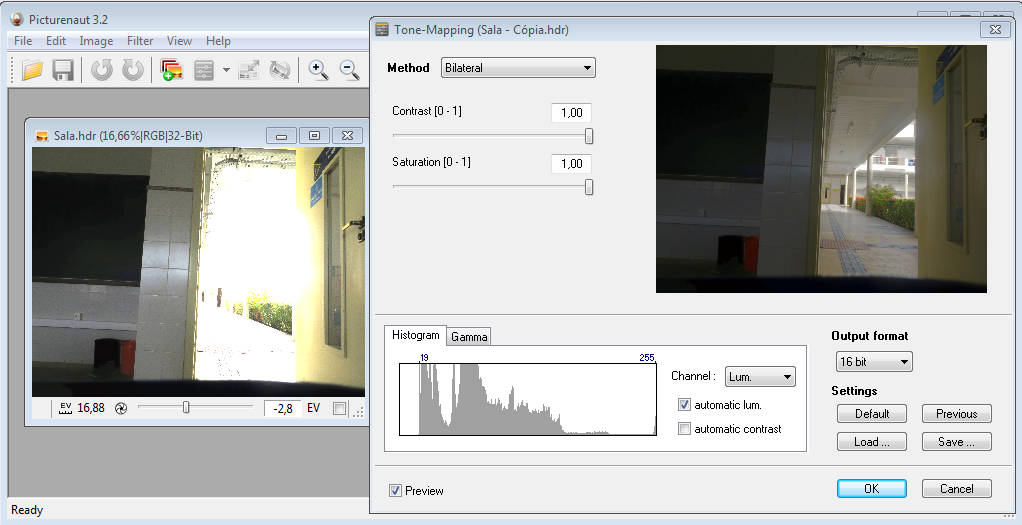
\includegraphics[height=8cm]{salaToneMapped}
  \caption{Exemplo de imagem HDR tonemapped.}
  \label{figExemploSFM}
\end{figure}
\section{Proposta para Melhoria na Aquisição dos Pontos de Interesse} \label{pontosProposta}
\subsection{Base de Imagens e Visualização} \label{pontosBaseImg}
\section{Resultados e Discussões} \label{pontosResultados}

Ao aplicar o método de geração de imagens HDR proposto por Sen~\etal~\cite{hdrMovimento} sobre as imagens da base de dados, notou-se que em algumas delas foram gerados artefatos antes não existentes. A Figura \ref{figResTonemap} mostra a versão \textit{tonemapped} das imagens HDR geradas.

\begin{figure}[H]
  \centering 
  \subfloat[Objeto visto de frente.]
  {
    \includegraphics[height=5cm]{toneMapping/PontosFrente}
    \label{figResTonemapA}
  }  
  \quad %espaco separador
  \subfloat[Objeto visto por baixo.]
  {
    \includegraphics[height=5cm]{toneMapping/PontosBaixo}
    \label{figResTonemapB}
  }
  \quad %espaco separador
  \subfloat[Objeto visto por cima.]
  {
    \includegraphics[height=5cm]{toneMapping/PontosCima}
    \label{figResTonemapC}
  }
  \quad %espaco separador
  \subfloat[Objeto visto pela direita.]
  {
    \includegraphics[height=5cm]{toneMapping/PontosDireita}
    \label{figResTonemapD}
  }
  \quad %espaco separador
  \subfloat[Objeto visto pela esquerda.]
  {
    \includegraphics[height=5cm]{toneMapping/PontosEsquerda}
    \label{figResTonemapE}
  }
  \caption{Imagens HDR \textit{tonemapped} da base de dados.}
  \label{figResTonemap}
\end{figure}

É visívels na Figuras \ref{figResTonemapA}, \ref{figResTonemapB}, e \ref{figResTonemapE}, apresença de distorções e no caso da Figura \ref{figResTonemapB} a presença de mais grades que o esperado. Provavelmente estes problemas foram gerados devido ao movimento existente entre as imagens LDR que geraram as respectivas imagens HDR.

Foi feito então a comparação da obtenção de nuvem de pontos utilizando imagens convencionais em relação às imagens \textit{tonemapped} obtidas. Ao gerar a nuvem de pontos utilizando o conjunto de imagens LDR mais bem expostas, citado na Seção \ref{pontosBaseImg}, foi obtido resultado melhor que ao utilizar as figuras HDR \ref{tonemapped}. A Tabela \ref{tabResultados} mostra a média de pontos de interesse que foram corretamente correspondidos entre as imagens, assim como o número de pontos 3D obtidos nas nuvens de pontos de cada abordagem. E a Figura \ref{figNuvemPontos} mostra as nuvens de pontos obtidas.

\begin{table}[H]
  \centering
  \caption{Resultados obtidos com a geração das nuvens de pontos.}
  \label{tabResultados}
  \begin{tabular}{l|l|l}
    \hline
               & Média de correspondência &  Número de pontos 3D \\
               & dos pontos de interesse  \\
               & por par de imagens       \\
    \hline
    Imagens LDR convencionais & 183,6 & 1262 \\
    \hline
    Imagens \textit{tonemapped} & 139,3 & 937 \\  
    \hline
  \end{tabular}
\end{table}

\begin{figure}[H]
  \centering 
  \subfloat[Obtida utilizando imagens LDR convencionais.]
  {
    \includegraphics[height=5cm]{nuvemPontos/Convencional}
    \label{figNuvemPontosA}
  }  
  \quad %espaco separador
  \subfloat[Obtida utilizando as imagens \textit{tonemapped} geradas.]
  {
    \includegraphics[height=5cm]{nuvemPontos/HDR}
    \label{figNuvemPontosB}
  }
  \caption{Nuvens de pontos obtidas utilizando o software VisualSFM.}
  \label{figNuvemPontos}
\end{figure}


Tendo em vista o resultado obtido com as imagens \textit{tonemapped}, optou-se por não dar continuidade ao processo proposto na Seção \ref{pontosProposta}. A justificativa disso é que por conta dos artefatos das imagens HDR geradas, ao realçá-las também haverá o realce dessas singularidades, levando a obtenção de pontos de interesse falsos e não úteis.

\chapter{Considerações Finais} \label{conclusao}

Com base nos resultados conclui-se que o uso de imagens HDR obtidas a partir de um conjunto de imagens LDR com diferentes tempos de exposição não se mostra uma alternativa viável para a geração de nuvens de pontos 3D, tendo em vista que as imagens LDR não são capturadas com uso de ferramentas profissionais como tripé.

Os resultados mostraram que as imagens HDR \textit{tonemapped}, que deveriam possuir mais informações do ambiente em relação a uma LDR comum, geraram nuvem de pontos de qualidade inferior à nuvem de pontos obtida utilizando imagens LDR convencionais. O fator que se mostrou limitante para o processo foi a inerente movimentação da câmera entre a captura das imagens LDR, que compuseram as imagens HDR. O fato das imagens não serem alinhadas acabou por gerar artefatos nas imagens HDR o que dificultou o processo de obtenção dos pontos 3D ao invés de melhorá-lo.

Como trabalhos futuros pode-se analisar o processo abordado neste trabalho utilizando-se de ferramentas profissionais que possibilitem a captura de imagens em diferentes tempos de exposição sem que haja movimento entre duas capturas.





%%%%%%%%%%%%%%%%%%%%%%%%%%%%%%%%%%%%%%%%%%%%%%%%%%%%%%%%%%%%%%%%%%%%%%%%%%%%%%%%%%%%%%%%%
%% Troca do termo Bibliografia para Referencia.
%% Adicao da pagina da Referencia no Sumario
\addcontentsline{toc}{chapter}{Referências}
\renewcommand{\bibname}{REFERÊNCIAS} 

%%%%%%%%%%%%%%%%%%%%%%%%%%%%%%%%%%%%%%%%%%%%%%%%%%%%%%%%%%%%%%%%%%%%%%%%%%%%%%%%%%%%%%%%%%%%%%%%
%% Bibliografia
%% Coloque suas referencias no arquivo referencias.bib
\bibliographystyle{plain} % estilo de bibliografia   plain,unsrt,alpha,abbrv.
%\nocite{*} %coloca todas as referências
\bibliography{Documentos/Referencias} % arquivos com as entradas bib.

%%%%%%%%%%%%%%%%%%%%%%%%%%%%%%%%%%%%%%%%%%%%%%%%%%%%%%%%%%%%%%%%%%%%%%%%%%%%%%%%%%%%%%%%%%%%%%%%%
%% Apendice
%% Caso seja necessario algum apendice, descomente a linha abaixo e crie o arquivo apendices.tex.
\appendix
%\input{apendices}

\end{document}